
% I seguenti commenti speciali impostano:
% 1. 
% 2. PDFLaTeX come motore di composizione;
% 3. tesi.tex come documento principale;
% 4. il controllo ortografico italiano per l'editor.

% !TEX encoding = UTF-8
% !TEX TS-program = pdflatex
% !TEX root = tesi.tex
% !TEX spellcheck = it-IT

\documentclass[12pt,                    % corpo del font principale
               a4paper,                 % carta A4
               twoside,                 % impagina per fronte-retro
               openright,               % inizio capitoli a destra
               english,                 
               italian,                 
               ]{book}    

%**************************************************************
% Importazione package
%************************************************************** 

%\usepackage{amsmath,amssymb,amsthm}    % matematica

\usepackage[T1]{fontenc}                % codifica dei font:
                                        % NOTA BENE! richiede una distribuzione *completa* di LaTeX

\usepackage[utf8]{inputenc}             % codifica di input; anche [latin1] va bene
                                        % NOTA BENE! va accordata con le preferenze dell'editor

\usepackage[english, italian]{babel}    % per scrivere in italiano e in inglese;
                                        % l'ultima lingua (l'italiano) risulta predefinita

\usepackage{bookmark}                   % segnalibri

\usepackage{caption}                    % didascalie

\usepackage{chngpage,calc}              % centra il frontespizio

\usepackage{csquotes}                   % gestisce automaticamente i caratteri (")

\usepackage{emptypage}                  % pagine vuote senza testatina e piede di pagina

\usepackage{epigraph}			% per epigrafi

\usepackage{eurosym}                    % simbolo dell'euro

%\usepackage{indentfirst}               % rientra il primo paragrafo di ogni sezione

\usepackage{graphicx}                   % immagini

\usepackage{hyperref}                   % collegamenti ipertestuali

\usepackage[binding=5mm]{layaureo}      % margini ottimizzati per l'A4; rilegatura di 5 mm

\usepackage{listings}                   % codici

\usepackage{microtype}                  % microtipografia

\usepackage{mparhack,fixltx2e,relsize}  % finezze tipografiche

\usepackage{nameref}                    % visualizza nome dei riferimenti                                      

\usepackage[font=small]{quoting}        % citazioni

\usepackage{subfig}                     % sottofigure, sottotabelle

\usepackage[italian]{varioref}          % riferimenti completi della pagina

\usepackage[dvipsnames]{xcolor}         % colori

\usepackage{booktabs}                   % tabelle                                       
\usepackage{tabularx}                   % tabelle di larghezza prefissata                                    
\usepackage{longtable}                  % tabelle su più pagine                                        
\usepackage{ltxtable}                   % tabelle su più pagine e adattabili in larghezza

\usepackage[toc, acronym]{glossaries}   % glossario
                                        % per includerlo nel documento bisogna:
                                        % 1. compilare una prima volta tesi.tex;
                                        % 2. eseguire: makeindex -s tesi.ist -t tesi.glg -o tesi.gls tesi.glo
                                        % 3. eseguire: makeindex -s tesi.ist -t tesi.alg -o tesi.acr tesi.acn
                                        % 4. compilare due volte tesi.tex.

\usepackage[backend=biber,style=verbose-ibid,hyperref,backref]{biblatex}
                                        % eccellente pacchetto per la bibliografia; 
                                        % produce uno stile di citazione autore-anno; 
                                        % lo stile "numeric-comp" produce riferimenti numerici
                                        % per includerlo nel documento bisogna:
                                        % 1. compilare una prima volta tesi.tex;
                                        % 2. eseguire: biber tesi
                                        % 3. compilare ancora tesi.tex.

%**************************************************************
% file contenente le impostazioni della tesi
%**************************************************************

%**************************************************************
% Frontespizio
%**************************************************************

% Autore
\newcommand{\myName}{Gianluca Travasci}                                    

\newcommand{\myTitle}{Sviluppo e miglioramento del software ERP F12 - Gestionale per protocolli}

% Tipo di tesi                   
\newcommand{\myDegree}{Tesi di laurea triennale}

% Università             
\newcommand{\myUni}{Università degli Studi di Padova}

% Facoltà       
\newcommand{\myFaculty}{Corso di Laurea in Informatica}

% Dipartimento
\newcommand{\myDepartment}{Dipartimento di Matematica "Tullio Levi-Civita"}

% Titolo del relatore
\newcommand{\profTitle}{Prof.}

% Relatore
\newcommand{\myProf}{Claudio Enrico Palazzi}

% Luogo
\newcommand{\myLocation}{Padova}

% Anno accademico
\newcommand{\myAA}{2017-2018}

% Data discussione
\newcommand{\myTime}{ 18 Dicembre 2018}

% Azienda
\newcommand{\myAzienda}{Gestiware S.r.l.}

% Tutor
\newcommand{\myTutor}{Matteo Orlando}


%**************************************************************
% Impostazioni di impaginazione
% see: http://wwwcdf.pd.infn.it/AppuntiLinux/a2547.htm
%**************************************************************

\setlength{\parindent}{14pt}   % larghezza rientro della prima riga
\setlength{\parskip}{0pt}   % distanza tra i paragrafi


%**************************************************************
% Impostazioni di biblatex
%**************************************************************
\bibliography{bibliografia} % database di biblatex 

\defbibheading{bibliography} {
    \cleardoublepage
    \phantomsection 
    \addcontentsline{toc}{chapter}{\bibname}
    \chapter*{\bibname\markboth{\bibname}{\bibname}}
}

\setlength\bibitemsep{1.5\itemsep} % spazio tra entry

\DeclareBibliographyCategory{opere}
\DeclareBibliographyCategory{web}

\addtocategory{opere}{womak:lean-thinking}
\addtocategory{web}{site:agile-manifesto}

\defbibheading{opere}{\section*{Riferimenti bibliografici}}
\defbibheading{web}{\section*{Siti Web consultati}}


%**************************************************************
% Impostazioni di caption
%**************************************************************
\captionsetup{
    tableposition=top,
    figureposition=bottom,
    font=small,
    format=hang,
    labelfont=bf
}

%**************************************************************
% Impostazioni di glossaries
%**************************************************************

%**************************************************************
% Acronimi
%**************************************************************
\renewcommand{\acronymname}{Acronimi e abbreviazioni}

\newacronym[description={\glslink{apig}{Application Program Interface}}]
    {api}{API}{Application Program Interface}

\newacronym[description={\glslink{umlg}{Unified Modeling Language}}]
    {uml}{UML}{Unified Modeling Language}

%**************************************************************
% Glossario
%**************************************************************
%\renewcommand{\glossaryname}{Glossario}

\newglossaryentry{PHP}
{
    name=\glslink{PHP}{PHP},
    text=Application Program Interface,
    sort=api,
    description={in informatica con il termine \emph{Application Programming Interface API} (ing. interfaccia di programmazione di un'applicazione) si indica ogni insieme di procedure disponibili al programmatore, di solito raggruppate a formare un set di strumenti specifici per l'espletamento di un determinato compito all'interno di un certo programma. La finalità è ottenere un'astrazione, di solito tra l'hardware e il programmatore o tra software a basso e quello ad alto livello semplificando così il lavoro di programmazione}
}

\newglossaryentry{umlg}
{
    name=\glslink{uml}{UML},
    text=UML,
    sort=uml,
    description={in ingegneria del software \emph{UML, Unified Modeling Language} (ing. linguaggio di modellazione unificato) è un linguaggio di modellazione e specifica basato sul paradigma object-oriented. L'\emph{UML} svolge un'importantissima funzione di ``lingua franca'' nella comunità della progettazione e programmazione a oggetti. Gran parte della letteratura di settore usa tale linguaggio per descrivere soluzioni analitiche e progettuali in modo sintetico e comprensibile a un vasto pubblico}
}
 % database di termini
\makeglossaries


%**************************************************************
% Impostazioni di graphicx
%**************************************************************
\graphicspath{{immagini/}} % cartella dove sono riposte le immagini


%**************************************************************
% Impostazioni di hyperref
%**************************************************************
\hypersetup{
    %hyperfootnotes=false,
    %pdfpagelabels,
    %draft,	% = elimina tutti i link (utile per stampe in bianco e nero)
    colorlinks=true,
    linktocpage=true,
    pdfstartpage=1,
    pdfstartview=FitV,
    % decommenta la riga seguente per avere link in nero (per esempio per la stampa in bianco e nero)
    %colorlinks=false, linktocpage=false, pdfborder={0 0 0}, pdfstartpage=1, pdfstartview=FitV,
    breaklinks=true,
    pdfpagemode=UseNone,
    pageanchor=true,
    pdfpagemode=UseOutlines,
    plainpages=false,
    bookmarksnumbered,
    bookmarksopen=true,
    bookmarksopenlevel=1,
    hypertexnames=true,
    pdfhighlight=/O,
    %nesting=true,
    %frenchlinks,
    urlcolor=webbrown,
    linkcolor=RoyalBlue,
    citecolor=webgreen,
    %pagecolor=RoyalBlue,
    %urlcolor=Black, linkcolor=Black, citecolor=Black, %pagecolor=Black,
    pdftitle={\myTitle},
    pdfauthor={\textcopyright\ \myName, \myUni, \myFaculty},
    pdfsubject={},
    pdfkeywords={},
    pdfcreator={pdfLaTeX},
    pdfproducer={LaTeX}
}

%**************************************************************
% Impostazioni di itemize
%**************************************************************
%\renewcommand{\labelitemi}{$\ast$}

%\renewcommand{\labelitemi}{$\bullet$}
%\renewcommand{\labelitemii}{$\cdot$}
%\renewcommand{\labelitemiii}{$\diamond$}
%\renewcommand{\labelitemiv}{$\ast$}


%**************************************************************
% Impostazioni di listings
%**************************************************************
\lstset{
    language=[LaTeX]Tex,%C++,
    keywordstyle=\color{RoyalBlue}, %\bfseries,
    basicstyle=\small\ttfamily,
    %identifierstyle=\color{NavyBlue},
    commentstyle=\color{Green}\ttfamily,
    stringstyle=\rmfamily,
    numbers=none, %left,%
    numberstyle=\scriptsize, %\tiny
    stepnumber=5,
    numbersep=8pt,
    showstringspaces=false,
    breaklines=true,
    frameround=ftff,
    frame=single
} 


%**************************************************************
% Impostazioni di xcolor
%**************************************************************
\definecolor{webgreen}{rgb}{0,.5,0}
\definecolor{webbrown}{rgb}{.6,0,0}


%**************************************************************
% Altro
%**************************************************************

\newcommand{\omissis}{[\dots\negthinspace]} % produce [...]

% eccezioni all'algoritmo di sillabazione
\hyphenation
{
    ma-cro-istru-zio-ne
    gi-ral-din
}

\newcommand{\sectionname}{sezione}
\addto\captionsitalian{\renewcommand{\figurename}{Figura}
                       \renewcommand{\tablename}{Tabella}}

\newcommand{\glsfirstoccur}{\ap{{[g]}}}

\newcommand{\intro}[1]{\emph{\textsf{#1}}}

%**************************************************************
% Environment per ``rischi''
%**************************************************************
\newcounter{riskcounter}                % define a counter
\setcounter{riskcounter}{0}             % set the counter to some initial value

%%%% Parameters
% #1: Title
\newenvironment{risk}[1]{
    \refstepcounter{riskcounter}        % increment counter
    \par \noindent                      % start new paragraph
    \textbf{\arabic{riskcounter}. #1}   % display the title before the 
                                        % content of the environment is displayed 
}{
    \par\medskip
}

\newcommand{\riskname}{Rischio}

\newcommand{\riskdescription}[1]{\textbf{\\Descrizione:} #1.}

\newcommand{\risksolution}[1]{\textbf{\\Soluzione:} #1.}

%**************************************************************
% Environment per ``use case''
%**************************************************************
\newcounter{usecasecounter}             % define a counter
\setcounter{usecasecounter}{0}          % set the counter to some initial value

%%%% Parameters
% #1: ID
% #2: Nome
\newenvironment{usecase}[2]{
    \renewcommand{\theusecasecounter}{\usecasename #1}  % this is where the display of 
                                                        % the counter is overwritten/modified
    \refstepcounter{usecasecounter}             % increment counter
    \vspace{10pt}
    \par \noindent                              % start new paragraph
    {\large \textbf{\usecasename #1: #2}}       % display the title before the 
                                                % content of the environment is displayed 
    \medskip
}{
    \medskip
}

\newcommand{\usecasename}{UC}

\newcommand{\usecaseactors}[1]{\textbf{\\Attori Principali:} #1. \vspace{4pt}}
\newcommand{\usecasepre}[1]{\textbf{\\Precondizioni:} #1. \vspace{4pt}}
\newcommand{\usecasedesc}[1]{\textbf{\\Descrizione:} #1. \vspace{4pt}}
\newcommand{\usecasepost}[1]{\textbf{\\Postcondizioni:} #1. \vspace{4pt}}
\newcommand{\usecasealt}[1]{\textbf{\\Scenario Alternativo:} #1. \vspace{4pt}}

%**************************************************************
% Environment per ``namespace description''
%**************************************************************

\newenvironment{namespacedesc}{
    \vspace{10pt}
    \par \noindent                              % start new paragraph
    \begin{description} 
}{
    \end{description}
    \medskip
}

\newcommand{\classdesc}[2]{\item[\textbf{#1:}] #2}                     % file con le impostazioni personali

\begin{document}
%**************************************************************
% Materiale iniziale
%**************************************************************
\frontmatter
% !TEX encoding = UTF-8
% !TEX TS-program = pdflatex
% !TEX root = ../tesi.tex

%**************************************************************
% Frontespizio 
%**************************************************************
\begin{titlepage}

\begin{center}

\begin{LARGE}
\textbf{\myUni}\\
\end{LARGE}

\vspace{10pt}

\begin{Large}
\textsc{\myDepartment}\\
\end{Large}

\vspace{10pt}

\begin{large}
\textsc{\myFaculty}\\
\end{large}

\vspace{30pt}
\begin{figure}[htbp]
\begin{center}

\includegraphics[height=6cm]{logo-unipd}
\end{center}
\end{figure}
\vspace{30pt} 

\begin{LARGE}
\begin{center}
\textbf{Sviluppo e miglioramento del software ERP F12}\\
\end{center}
\end{LARGE}

\vspace{10pt} 

\begin{large}
\textsl{\myDegree}\\
\end{large}

\vspace{40pt} 

\begin{large}
\begin{flushleft}
\textit{Relatore}\\ 
\vspace{5pt} 
Prof. Claudio Enrico Palazzi
\end{flushleft}

\vspace{0pt} 

\begin{flushright}
\textit{Laureando}\\ 
\vspace{5pt} 
\myName 
\\
\textit{Matricola 1120260}
\end{flushright}
\end{large}

\vspace{30pt}

\line(1, 0){338} \\
\begin{normalsize}
\textsc{Anno Accademico \myAA}
\end{normalsize}

\end{center}
\end{titlepage} 
% !TEX encoding = UTF-8
% !TEX TS-program = pdflatex
% !TEX root = ../tesi.tex

%**************************************************************
% Colophon
%**************************************************************
\clearpage
\phantomsection
\thispagestyle{empty}

\hfill

\vfill

\noindent\myName: \textit{\myTitle,}
\myDegree,
\textcopyright\ \myTime.
% !TEX encoding = UTF-8
% !TEX TS-program = pdflatex
% !TEX root = ../tesi.tex

%**************************************************************
% Dedica
%**************************************************************
\cleardoublepage
\phantomsection
\thispagestyle{empty}
\pdfbookmark{Dedica}{Dedica}

\vspace*{3cm}

\begin{center}
Nel mondo nulla di grande è stato fatto senza passione. \\ \medskip
-- Georg Wilhelm Friedrich Hegel 
\end{center}

\medskip



% !TEX encoding = UTF-8
% !TEX TS-program = pdflatex
% !TEX root = ../tesi.tex

%**************************************************************
% Sommario
%**************************************************************
\cleardoublepage
\phantomsection
\pdfbookmark{Sommario}{Sommario}
\begingroup
\let\clearpage\relax
\let\cleardoublepage\relax
\let\cleardoublepage\relax

\chapter*{Sommario}

Il presente documento descrive il lavoro svolto durante il periodo di stage, della durata di 320 ore, dal laureando Gianluca Travasci presso l'azienda \myAzienda  di Pordenone (PN).
\\
\\
Lo scopo dello stage è stato quello di implementare al software F12, realizzato da \myAzienda, la possibilità di gestire, archiviare e configurare dei protocolli. Il suddetto lavoro è stato svolto per far fronte alla necessità di una cooperativa della zona di Pordenone di gestire in modo efficiente ed immediato ogni aspetto della protocollazione.
\\
\\
Gli obiettivi da raggiungere erano molteplici: in primo luogo era richiesto lo studio della proposta d'appalto per poi realizzare una breve analisi dei requisiti corredata da mockup da presentare all'azienda proponente.
In secondo luogo era richiesto lo studio del software F12 e del framework ad esso collegato per poi cominciare a lavorarci.\\
Infine era richiesta la realizzazione dell'infrastruttura base lato server, la realizzazione delle principali maschere lato client e l'interazione con il database mediante linguaggio SQL.

%\vfill
%
%\selectlanguage{english}
%\pdfbookmark{Abstract}{Abstract}
%\chapter*{Abstract}
%
%\selectlanguage{italian}

\endgroup			

\vfill


% !TEX encoding = UTF-8
% !TEX TS-program = pdflatex
% !TEX root = ../tesi.tex

%**************************************************************
% Ringraziamenti
%**************************************************************
\cleardoublepage
\phantomsection
\pdfbookmark{Ringraziamenti}{ringraziamenti}

\bigskip

\begingroup
\let\clearpage\relax
\let\cleardoublepage\relax
\let\cleardoublepage\relax

\chapter*{Ringraziamenti}

\noindent \textit{Innanzitutto, vorrei esprimere la mia gratitudine al Prof. \myProf, relatore della mia tesi, per l'aiuto e il sostegno fornitomi durante la stesura del lavoro.}\\

\noindent \textit{Un sincero grazie al mio tutor aziendale Matteo Orlando per avermi seguito in questo percorso e per le conoscenze trasmesse.}\\

\noindent \textit{Desidero ringraziare inoltre i colleghi di Gestiware S.r.l., con i quali ho condiviso questo ultimo periodo, per aver contribuito a rendere lo stage una piacevole esperienza.}\\

\noindent \textit{Desidero ringraziare con affetto i miei genitori per il sostegno, il grande aiuto e per essermi stati vicini in ogni momento durante gli anni di studio.}\\

\noindent \textit{Ringrazio Laura, la mia ragazza, per i bellissimi momenti passati insieme e per avermi sempre sostenuto in questo percorso.}\\

\noindent \textit{Ho desiderio di ringraziare poi i miei amici per tutti i bellissimi anni passati insieme e le mille avventure vissute.}\\
\bigskip

\noindent\textit{\myLocation, \myTime}
\hfill \myName

\endgroup


% !TEX encoding = UTF-8
% !TEX TS-program = pdflatex
% !TEX root = ../tesi.tex

%**************************************************************
% Indici
%**************************************************************
\cleardoublepage
\pdfbookmark{\contentsname}{tableofcontents}
\setcounter{tocdepth}{2}
\tableofcontents
%\markboth{\contentsname}{\contentsname} 
\clearpage

\begingroup 
    \let\clearpage\relax
    \let\cleardoublepage\relax
    \let\cleardoublepage\relax
    %*******************************************************
    % Elenco delle figure
    %*******************************************************    
    \phantomsection
    \pdfbookmark{\listfigurename}{lof}
    \listoffigures

    \vspace*{2ex}

    %*******************************************************
    % Elenco delle tabelle
    %*******************************************************
    \phantomsection
    \pdfbookmark{\listtablename}{lot}
    \listoftables
        
    \vspace*{2ex}
    
    %*******************************************************
    % Elenco dei Listing
    %*******************************************************
    \phantomsection
    %\pdfbookmark{\listlistname}{lot}
    \lstlistoflistings
        
    \vspace*{2ex}
    
\endgroup

\cleardoublepage

\cleardoublepage

%**************************************************************
% Materiale principale
%**************************************************************
\mainmatter
% !TEX encoding = UTF-8
% !TEX TS-program = pdflatex
% !TEX root = ../tesi.tex

%**************************************************************
\chapter{Introduzione}
\label{cap:introduzione}
%**************************************************************

Questo capitolo ha lo sopo di fornire una breve descrizione dell'azienda ospitante, della struttura del seguente documento e delle norme utilizzate per la stesura dello stesso.\\


%\noindent Esempio di utilizzo di un termine nel glossario \\
%\gls{api}. \\

%\noindent Esempio di citazione in linea \\
%\cite{site:agile-manifesto}. \\

%\noindent Esempio di citazione nel pie' di pagina \\
%citazione\footcite{womak:lean-thinking} \\

%**************************************************************
\section{L'azienda}
\subsection{Profilo aziendale}
    Gestiware Srl è una \emph{\textit{software house}}\glsfirstoccur che realizza soluzioni informatiche su specifica e sistemi di \emph{\textit{software integration}}\glsfirstoccur.
    \\
    Il prodotto di riferimento è il software gestionale F12 realizzato e sviluppato da Gestiware S.r.l, corredato da diverse estensioni dipartimentali integrate allo stesso.
    \\
    L'obiettivo è quello di fornire ai clienti la consulenza necessaria e i prodotti software atti al miglioramento del loro sistema informatico e organizzativo.
    \begin{figure}[!h] 
        \centering 
        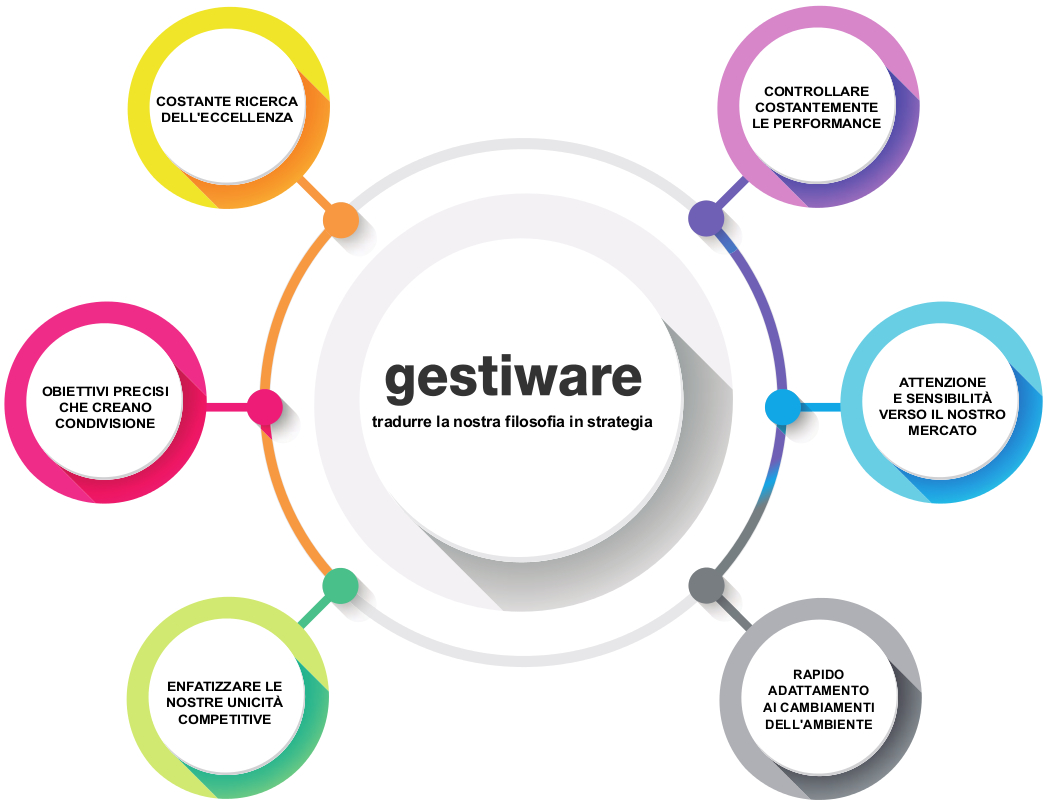
\includegraphics[width=1\columnwidth]{immagini/505-TEST4.jpg}
        \caption{Presentazione azienda}
    \end{figure}
    \newpage
\subsection{Servizi offerti}
    L'attività aziendale riguarda tre aree principali: 
    \begin{itemize}
        \item prodotti software;
        
        \item consulenze architetturali e organizzative;
        
        \item realizzazioni di progetti enterprise.
    \end{itemize}
    F12 è un software \emph{ERP}\glsfirstoccur completo in grado di supportare l'azienda in tutte le sue principali attività: amministrazione, flusso acquisti e vendite e supervisione della produzione.
    \\
    F12 unisce l'esperienza raccolta dai soci fondatori nel settore alle tecnologie e modalità operative odierne, garantendo stabilità e flessibilità nella gestione dei dati aziendali.
    \\
    Da una linea di sviluppo principale ed orientata ad un'azienda manifatturiera in
    generale, sono state derivate personalizzazioni specifiche per i vari settori produttivi, come ad esempio quello del mobile, chimico, servizi, cantieri eristica navale e da diporto, alimentare, cartotecnico, ecc.
    \\
    Oltre alle personalizzazioni orientate al settore produttivo, Gestiware ha dedicato un
    significativo periodo di tempo allo studio e realizzazione di interfacce di comunicazione fra F12 ed altri software di interesse aziendale. 
    \\
    Nell'ambito del sistema ERP, la ricerca si è focalizzata sul miglioramento delle tecniche
    tradizionali di gestione del magazzino e della produzione, offrendo un set di strumenti
    innovativi che riducono notevolmente i costi di gestione in questi ambiti, sia in termini
    monetari che computazionali.
    
\subsection{Vantaggi aziendali}
Per Gestiware S.r.l. i percorsi di tirocinio, sia universitari che per la scuola secondaria di secondo grado, sono fondamentali in quanto permettono all'azienda di entrare in contatto con ragazzi ed istituti con l'obiettivo di proporre un futuro impiego o collaborazione.

%**************************************************************
\section{Convenzioni tipografiche}
Nei paragrafi di questa sezione sono riportate le norme tipografiche adottate per la stesura del seguente testo. Lo scopo di tali norme è quello di produrre un documento rigorosamente formale e coerente.
\\
\\
\textbf{Glossario.} Per la prima occorrenza dei termini riportati nel glossario, situato alla fine del presente documento, viene utilizzata la seguente nomenclatura: \emph{parola}\glsfirstoccur;
\\
\\
\textbf{Elenchi puntati.} Gli elenchi puntati servono ad esprimere un concetto in modo sintetico e strutturato, evitando di utilizzare uno stile troppo narrativo, che mal si adatta in documenti di tipo tecnico-informativo. \newline
Ogni voce nell'elenco puntato inizia con la lettera minuscola (tranne dove è necessario la lettera maiuscola, per esempio con nomi di attività) e finisce con un punto e virgola, ad eccezione dell'ultima, che si conclude con un punto.\newline
Se l'elenco ha l'obiettivo di descrivere punti salienti, allora il nome del termine va scritto in grassetto, con la prima lettera maiuscola e se è presente la relativa descrizione va inserita dopo i due punti. 
\\
\\
\textbf{Stile del testo}
\begin{itemize}
    \item \textbf{Grassetto:} verrà usato per titoli e per elementi che riassumono il contenuto in un elenco puntato, come in questo caso con la parola "Grassetto";
    
    \item \textbf{Corsivo:} verrà usato per citazioni, abbreviazioni e termini rilevanti da evidenziare;
    
    \item \textbf{Maiuscolo:} verrà usato per acronimi o per nomi che lo richiedono.
    
    \item \textbf{Virgolette:} verranno usate per citazioni, riferimenti a frasi o parole riportate precedentemente nel testo, nomi di documenti, voci di menù o voci di pulsanti da premere.
\end{itemize}




%**************************************************************
\section{Struttura del documento}

\begin{description}
    \item Il secondo capitolo, {\hyperref[cap:descrizione-stage]{Descrizione dello stage}}, riporta una breve descrizione dei possibili rischi, le modalità di svolgimento e la pianificazione dell'attività di stage svolta. Inoltre è riportata, a grandi linee, la richiesta dell'azienda proponente seguita dalla soluzione da me progettata per far fronte ad essa.
    
    \item Il terzo capitolo, {\hyperref[cap:protocollazione]{Protocollazione}}, approfondisce questa tematica fornendone una definizione, illustrandone la metodologia di registrazione di un protocollo e illustrandone la necessità di configurazione dei flussi applicativi.
    
    \item Il quarto capitolo, {\hyperref[cap:gestione-documentale]{Gestione documentale}}, approfondisce e illustra il software "F12 Documentale" fornitomi da Gestiware S.r.l. per una facile ed efficiente gestione dei documenti caricati attraverso il prodotto da me realizzato.
    
    \item Il quinto capitolo, {\hyperref[cap:progettazione-codifica]{Progettazione e codifica}}, approfondisce ogni singolo aspetto di queste due attività fondamentali da me svolte durante lo stage.
    
    \item Il sesto capitolo, {\hyperref[cap:verifica-validazione]{Verifica e validazione}}, descrive il lavoro svolto per quanto riguarda le attività di verifica e di validazione. 
    
    \item Il settimo capitolo, {\hyperref[cap:conclusioni]{Conclusioni}}, contiene un'analisi riassuntiva degli obiettivi raggiunti, delle conoscenze acquisite e le conclusioni sull'attività svolta.
\end{description}
% !TEX encoding = UTF-8
% !TEX TS-program = pdflatex
% !TEX root = ../tesi.tex

%**************************************************************
\chapter{Descrizione dello stage}
\label{cap:descrizione-stage}
%**************************************************************

\intro{Tale capitolo riporta una descrizione dei possibili rischi, la modalità di svolgimento, le problematiche da risolvere e le soluzioni proposte dell'attività di stage svolta. Viene inoltre riportata la pianificazione del lavoro e gli obiettivi da raggiungere al termine della stessa.}\\

%**************************************************************
\section{Analisi dei rischi}
Al fine di evitare rallentamenti dei periodi di lavoro è stata effettuata una breve analisi dei rischi, in modo da evitare le situazioni che portano alla creazione di eventi non pianificati, ove possibile. I rischi analizzati sono divisi per area di competenza, e per ognuno di essi è mostrata brevemente la strategia di mitigazione.
\begin{itemize}
    \item Livello tecnologico: 
        \begin{itemize}
            \item \textbf{Guasti hardware:} durante lo svolgimento dello stage è possibile che la strumentazione utilizzata, in particolare i computer assegnati, possano incorrere in guasti hardware, rischiando così di causare rallentamenti e perdita del lavoro.
            \\
            Per evitare questo evento verrà regolarmente caricato il materiale su una directory di uno dei server dell'azienda;
            
            \item \textbf{Linguaggio di programmazione poco padroneggiato:} durante lo svolgimento dello stage è richiesto l'utilizzo di \emph{PHP}\glsfirstoccur, linguaggio che non ho usato spesso nella mia carriera universitaria. Questo fatto potrebbe portare a ritardi o a difficoltà nello svolgimento del progetto. 
            \\
            Per far fronte a tale problematica studierò autonomamente le basi del linguaggio per poter affrontare con meno difficoltà il primo periodo di codifica;
            
            \item \textbf{Framework aziendale sconosciuto:} l'utilizzo di un \emph{framework}\glsfirstoccur realizzato da Gestiware S.r.l. e a me completamente sconosciuto potrebbe portare a ritardi o a difficoltà nello svolgimento del progetto.
            \\
             Tuttavia, grazie al periodo di apprendimento pianificato nella prima fase dello stage, e grazie alla presenza di personale esperto con cui confrontarsi, questo rischio non dovrebbe presentarsi;
        \end{itemize}
    \item Livello dei requisiti:
        \begin{itemize}
            \item \textbf{Incomprensioni e scelte non ottimali:} può accadere che alcune attività da svolgere siano fraintese o valutate erroneamente, causando la realizzazione di un prodotto non consono alle aspettative dell'azienda. Per mitigare questo rischio, ogni giorno avviene un incontro con il tutor aziendale per valutare il lavoro svolto e chiarire eventuali dubbi.
        \end{itemize}
\end{itemize}



%**************************************************************
\section{Modalità di svolgimento}
L’attività di stage è stata svolta presso la sede dell'azienda per favorire l’interazione dello studente con il tutor e per affacciarlo alla realtà di un team di sviluppo aziendale.\\
È stata quindi data la possibilità di relazionarsi con professionisti esperti ed essere supportato al meglio in caso di problematiche di realizzazione del progetto e di confrontarsi con il tutor per qualsiasi problematica.\\
L’organizzazione settimanale del lavoro è stata invece gestita tramite dei meeting, sempre con il tutor aziendale, atti a definire lo stato di avanzamento delle attività assegnate e rivedere in tempo reale gli obiettivi settimanali raggiunti o da raggiungere.\\
I risultati sono stati valutati mensilmente in base alla quantità di requisiti soddisfatti e alla qualità del prodotto realizzato.\\
L’orario lavorativo è stato il seguente: dal lunedì al venerdì, dalle 8:30 alle 18:00, con pausa pranzo dalle 12:30 alle 14:00.

%**************************************************************
\section{Pianificazione del lavoro}
La seguente sezione mostra, mediante \emph{diagramma di Gantt}\glsfirstoccur, la distribuzione temporale di ogni singola attività svolta durante il periodo di stage.

\begin{figure}[!h] 
    \centering 
    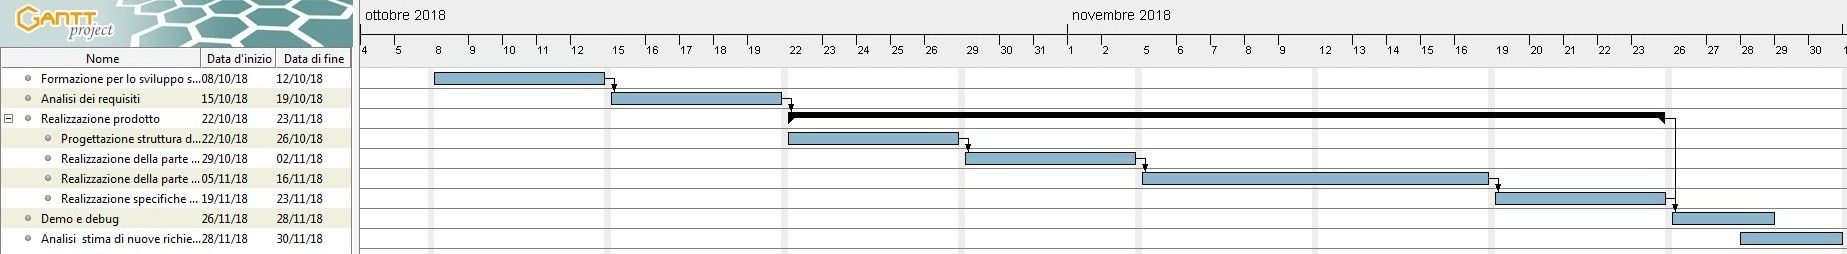
\includegraphics[width=1\columnwidth]{immagini/gantt.png} 
    \caption{Diagramma di Gantt - Attività svolte}
\end{figure}
%**************************************************************
\section{Problema della proponente}
In seguito all'incontro svoltosi in data 6 marzo tra i responsabili di Gestiware S.r.l e il responsabile dell'azienda proponente (Il nome dell'azienda o del responsabile non verranno mai citati per motivi di privacy) è risaltata l'esigenza di quest'ultima di avere un applicativo web in grado di gestire i protocolli in ingresso ed in uscita presso la suddetta. 
\\
Con "gestione di protocolli" si intende tutta l'attività svolta dagli operatori sui documenti in ingresso ed in uscita dall'azienda stessa.
\\
Le principali attività da svolgere sono:
\begin{itemize}
    \item Protocollare il documento, ossia:
        \begin{itemize}
            \item assegnare un identificativo univoco alfanumerico;
            
            \item assegnare un registro di appartenenza per una facile archiviazione;
            
            \item assegnare il documento ad un proprietario.
        \end{itemize}
    \item Smistare il documento al personale interno o anche esterno.
\end{itemize}
Questo tipo di operazioni vengono svolte, per ora, con diversi passaggi manuali, con la scrittura di mail con allegati precedentemente scansionati e/o salvati; quello che manca è un'automatizzazione di questi passaggi e un iter omogeneo che tracci tutto lo storico del protocollo.
\\
È stata inoltre esposta l'esigenza di gestire la privacy dei protocolli in quanto al suo interno sono contenuti dati sensibili di persone e/o aziende. 
%**************************************************************

\section{Analisi dei requisiti}
Tenuto conto dei vincoli elencati nei punti precedenti, per prima cosa si è eseguita un'analisi dei requisiti. Per fare ciò, è stata effettuata una fase di \emph{brainstorming}\glsfirstoccur, congiuntamente con il tutor aziendale, per stabilire quali fossero le feature da implementare e che priorità avrebbe dovuto avere ognuna di esse. Dopo questo primo brainstorming, lo stagista ha proceduto alla stesura del documento di analisi dei requisiti, iniziando con la realizzazione dei diagrammi \emph{UML}\glsfirstoccur che descrivessero tramite casi d'uso le interazioni dell'utente con il sistema.

\subsection{Funzionalità del prodotto}
Le funzionalità principali che l'applicativo web deve avere sono:
\begin{itemize}
        \item solo gli utenti dotati di credenziali di accesso potranno avere accesso all'applicazione web;
        
        \item ad un utente base è consentita la gestione dei protocolli da lui inseriti e a lui assegnati;
        
        \item ad un supervisore è consentita la gestione di tutti i protocolli;
        
        \item si dovrà fornire la possibilità di protocollare un documento in ingresso o in uscita, ossia assegnarne un identificativo, un registro di appartenenza e un "proprietario";
        
        \item deve essere possibile la registrazione di un nuovo contatto;
        
        \item deve esserci la possibilità di stampare il registro dei protocolli;

        \item deve esserci la possibilità di filtrare la lista di protocolli mediante tutti i campi visibili;
        
        \item deve esserci la possibilità di filtrare la lista di protocolli mediante l'utilizzo di scanner di barcode;
        
        \item deve esserci la possibilità di smistare mediante mail i protocolli;

        \item deve esserci la possibilità di inserire commenti e di avere lo storico delle attività;
        
        \item deve esserci la possibilità di configurare le tipologie di protocolli.
    \end{itemize}

\subsection{Casi d'uso}
\subsubsection{Classificazione dei casi d'uso}
Ogni caso d'uso sarà rappresentato con il seguente formalismo:
\begin{center}
    \textbf{UC[Codice]}
\end{center}
dove:\\
\textbf{Codice}: è un numero che identifica in modo univoco i casi d'uso.\\\\
Ogni caso d'uso, inoltre, deve essere descritto secondo la seguente specifica:
\begin{itemize}
    \item
    \textbf{ID}: è il codice identificativo del caso d'uso, di cui il formalismo sopra;
    \item
    \textbf{Attori}: gli attori coinvolti, sia principali sia secondari;
    \item
    \textbf{Descrizione}: breve descrizione del caso d'uso;
    \item
    \textbf{Pre-condizioni}: lo stato in cui si deve trovare il sistema affinché si verifichino le post-condizioni;
    \item
    \textbf{Post-condizioni}: le istruzioni che risultano vere dopo il verificarsi degli eventi del caso d'uso;
    \item
    \textbf{Scenario principale}: rappresenta il flusso principale degli eventi come elenco di azioni tra l'utente e il sistema;
    \item
    \textbf{Scenari alternativi}: casi d'uso esterni al flusso principale degli eventi che servono a gestire eventuali eccezioni o errori.
\end{itemize}
\newpage


\subsubsection{UC1 - Login}
    \label{UC1}
    \begin{figure}[!h] 
        \centering 
        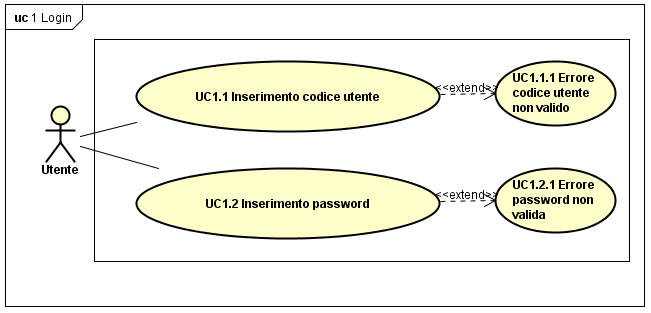
\includegraphics[width = 13cm]{immagini/UseCase/login.png} 
        \caption{UC1 Login}
    \end{figure}
    \textbf{Attori primari:} Utente non autenticato.
    \\
    \\
    \textbf{Descrizione:} L'attore vuole accedere al sistema.
    \\
    \\
    \textbf{Precondizione:} Il sistema visualizza il form per l'inserimento delle credenziali utente.
    \\
    \\
    \textbf{Postcondizione:}Il sistema ha autenticato l'attore, che viene rimandato alla pagina iniziale come utente autenticato.
    \\
    \\
    \textbf{Scenario principale:}
        \begin{itemize}
            \item L'attore deve inserire l'email (\hyperref[UC1.1]{UC1.1});
            \item L'attore deve inserire la password (\hyperref[UC1.2]{UC1.2});
        \end{itemize}
    \textbf{Scenari alternativi:} Il sistema visualizza un messaggio di errore relativo all'inserimento dei dati.


\subsubsection{UC1.1 - Inserimento codice utente}
    \label{UC1.1}
    \textbf{Attori primari:} Utente non autenticato.
    \\
    \\
    \textbf{Descrizione:} L'attore inserisce il proprio codice utente.
    \\
    \\
    \textbf{Precondizione:} Il sistema visualizza un campo in cui inserire il codice utente.
    \\
    \\
    \textbf{Postcondizione:} Il sistema ha l'informazione relativa all'utente.
    \\
    \\
    \textbf{Scenario principale:} L'attore deve inserire il proprio codice utente nell'apposita casella di testo.


\subsubsection{UC1.2 - Inserimento password}
    \label{UC1.2}
    \textbf{Attori primari:} Utente non autenticato.
    \\
    \\
    \textbf{Descrizione:} L'attore inserisce la propria password.
    \\
    \\
    \textbf{Precondizione:} Il sistema visualizza un campo in cui inserire la password.
    \\
    \\
    \textbf{Postcondizione:} Il sistema ha l'informazione relativa alla password.
    \\
    \\
    \textbf{Scenario principale:} L'attore deve inserire la propria password nell'apposita casella di testo.
    
    
    \subsubsection{UC1.3 - Errore "Email o Password errati"}
    \textbf{Attori primari:} Utente non autenticato.
    \\
    \\
    \textbf{Descrizione:} Il sistema visualizza un opportuno messaggio di errore relativo ai dati errati inseriti dall'attore.
    \\
    \\
    \textbf{Precondizione:} L'attore ha richiesto di effettuare la login tramite i propri dati.
    \\
    \\
    \textbf{Postcondizione:} Il sistema nega l'autenticazione visualizzando un messaggio di errore relativo ai dati inseriti.
    \\
    \\
    \textbf{Scenario principale:} Il sistema nega il login visualizzando un messaggio di errore relativo ai dati errati inseriti dall'attore.
    
    \newpage
    \subsubsection{UC}
    \label{UC}
    \begin{figure}[!h] 
        \centering 
        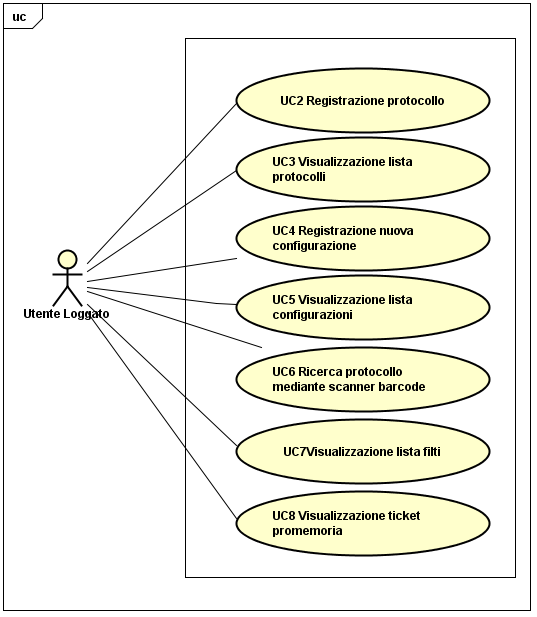
\includegraphics[width = 11cm]{immagini/UseCase/postlogin.png}
        \caption{UC Post Login}
    \end{figure}
    
    \textbf{Attori primari:} Utente loggato.
    \\
    \\
    \textbf{Descrizione:} L'utente loggato ha accesso a molteplici funzionalità.
    \\
    \\
    \textbf{Precondizione:} L'utente ha accesso al sistema.
    \\
    \\
    \textbf{Postcondizione:} Il sistema ha permesso di gestire le funzionalità di interesse dall'utente che si interfaccia con esso.
    \\
    \\
    \textbf{Scenario principale:} L'attore una volta autenticato può visualizzare le seguenti funzionalità:
            \begin{itemize}
                \item registrazione protocollo;
                \item Visualizzazione lista protocolli;
                \item registrazione nuova configurazione;
                \item visualizzazione lista configurazioni;
                \item ricerca protocollo mediante scanner di barcode;
                \item visualizzazione filtri;
                \item visualizzazione ticket promemoria.
            \end{itemize}

\subsubsection{UC2 Registrazione protocollo}
    \label{UC2}
    \begin{figure}[!h] 
        \centering 
        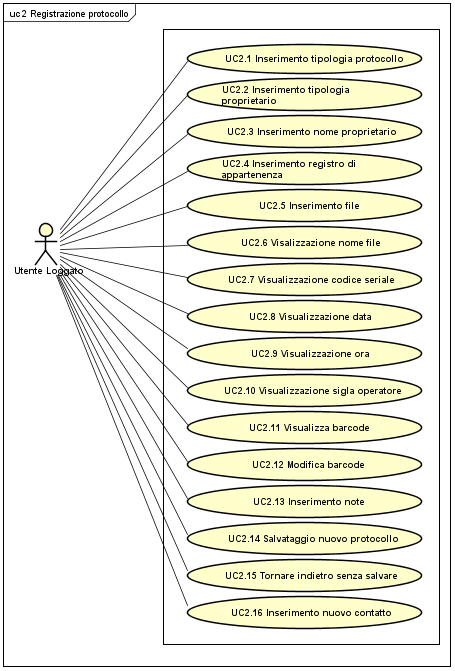
\includegraphics[width = 11cm]{immagini/UseCase/registrazioneprotocollo.png}
        \caption{UC2 Registrazione protocollo}
    \end{figure}
    
    \textbf{Attori primari:} Utente loggato.
    \\ 
    \\
    \textbf{Descrizione:} L'utente può registrare un nuovo protocollo compilando l'apposito form.
    \\
    \\
    \textbf{Precondizione:} L'utente ha accesso al form di registrazione di un nuovo protocollo.
    \\
    \\
    \textbf{Postcondizione:} Il sistema salva il protocollo regitrato mediante apposito form.
    \\
    \\
    \textbf{Scenario principale:} L'utente per registrare il nuovo protocollo deve inserire le seguenti informazioni o compiere le seguenti azioni:
            \begin{itemize}
                \item tipologia protocollo;
                \item tipologia proprietario;
                \item nome proprietario;
                \item registro di appartenenza ;
                \item file del documento da protocollare;
                \item nome del file;
                \item codice seriale del protocollo;
                \item data di registrazione;
                \item ora di registrazione;
                \item sigla operatore;
                \item barcode;
                \item modificare il codice a barre;
                \item salvare il protocollo;
                \item annullare la registrazione;
                \item inserire un nuovo contatto.
            \end{itemize}

\subsubsection{UC2.1 - Inserimento tipologia protocollo}
    \label{UC2.1}
    \textbf{Attori primari:} Utente loggato.
    \\
    \\
    \textbf{Descrizione:} Una volta selezionata una tipologia verranno stampati a video i campi \emph{metadato }\glsfirstoccur inseriti in fase di configurazione della tipologia.
    \\
    \\
    \textbf{Precondizione:} Il sistema visualizza un campo \textit{select} dove tutte le option sono le tipologie create dall'utente in \hyperref[UC4]{UC4}.
    \\
    \\
    \textbf{Postcondizione:} Il sistema stampa a video i campi metadato associati alla tipologia selezionata.
    \\
    \\
    \textbf{Scenario principale:} L'attore deve compilare tutti i campi metadato marcati come \textit{required}.
\newpage

\subsubsection{UC2.16 Inserimento nuovo contatto}
    \label{UC2.16}
    \begin{figure}[!h] 
        \centering 
        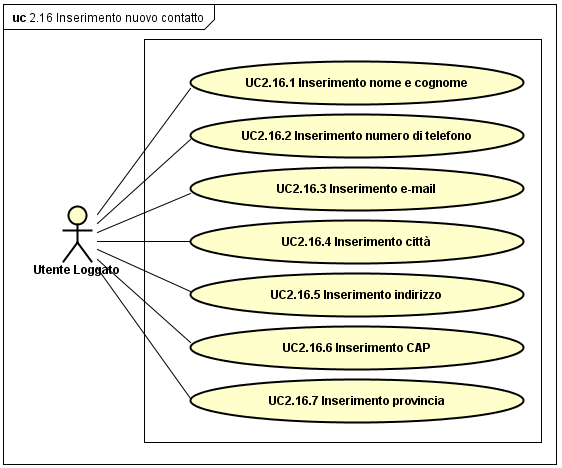
\includegraphics[width = 11cm]{immagini/UseCase/inserimentocontatto.png}
        \caption{UC2.16 Inserimento nuovo contatto}
    \end{figure}
    
    \textbf{Attori primari:} Utente loggato.
    \\ 
    \\
    \textbf{Descrizione:} L'utente se vuole assegnare il protocollo ad un proprietario non registrato nel database può registrarne uno nuovo con apposito form.
    \\
    \\
    \textbf{Precondizione:} L'utente seleziona "nuovo contatto" nella \textit{select} dedicata alla tipologia di proprietario.
    \\
    \\
    \textbf{Postcondizione:} Il sistema stampa a schermo il form di registrazione di un nuovo contatto.
    \\
    \\
    \textbf{Scenario principale:} L'utente per registrare il nuovo contatto deve inserire le seguenti informazioni:
            \begin{itemize}
                \item nome e cognome del contatto;
                \item numero di telefono del contatto;
                \item indirizzo e-mail;
                \item città;
                \item indirizzo;
                \item CAP;
                \item Provincia.
            \end{itemize}

\subsubsection{UC3 Visualizzazione lista protocolli}
    \label{UC3}
    \textbf{Attori primari:} Utente loggato.
    \\
    \\
    \textbf{Descrizione:} L'utente visualizza una lista di tutti i protocolli che deve visionare.
    \\
    \\
    \textbf{Precondizione:} Il sistema pende dal database tutti i protocolli di interesse.
    \\
    \\
    \textbf{Postcondizione:} Il sistema stampa a video tutti i protocolli.
    \\
    \\
    \textbf{Scenario principale:} L'attore può aprire uno qualsiasi dei protocolli della lista.
    \newpage

\subsubsection{UC3.1 Visualizzazione singolo protocollo}
    \label{UC3.1}
    \begin{figure}[!h] 
        \centering 
        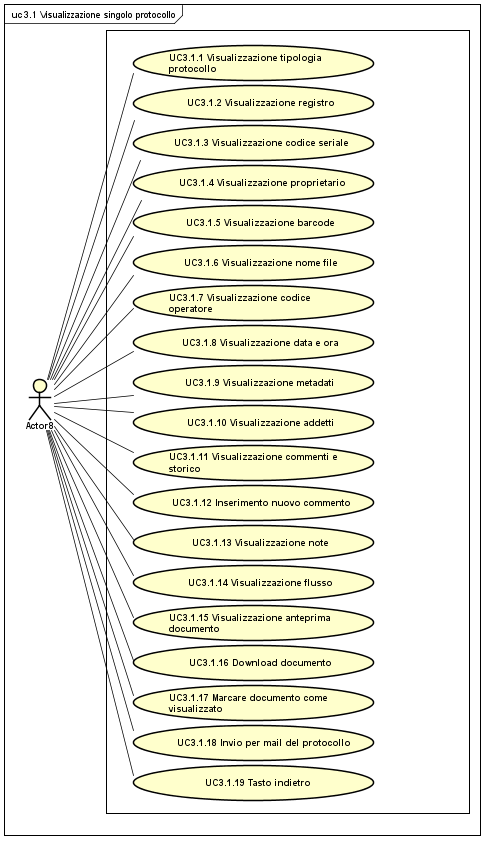
\includegraphics[width = 11cm]{immagini/UseCase/dettaglioprotocollo.png}
        \caption{UC3.1 Visualizzazione singolo protocollo}
    \end{figure}
    
    \textbf{Attori primari:} Utente loggato.
    \\ 
    \\
    \textbf{Descrizione:} L'utente apre la pagina di dettaglio di un singolo protocollo e ne visualizza le informazioni.
    \\
    \\
    \textbf{Precondizione:} L'utente seleziona uno dei protocolli nella lista descritta in \hyperref[UC3]{UC3}.
    \\
    \\
    \textbf{Postcondizione:} Il sistema stampa a schermo le informazioni riguardanti il protocollo selezionato dall'utente.
    \\
    \\
    \textbf{Scenario principale:} L'utente può:
            \begin{itemize}
                \item visualizzare la tipologia protocollo;
                \item visualizzare il registro di appartenenza;
                \item visualizzare il codice seriale;
                \item visualizzare il proprietario a cui è intestato il protocollo;
                \item visualizzare il barcode;
                \item visualizzare il nome file;
                \item visualizzare il codice operatore;
                \item visualizzare la data e ora;
                \item visualizzare i metadati corrispondenti alla tipologia;
                \item visualizzare gli operatori addetti all'elaborazione della tipologia di cui fa parte il protocollo;
                \item visualizzare i commenti e lo storico del protocollo;
                \item inserire un nuovo commento;
                \item visualizzare le note riguardanti il protocollo;
                \item visualizzare il flusso del protocollo;
                \item visualizzare l'anteprima del documento caricato;
                \item premere il tasto download documento;
                \item premere il tasto per marcare come visionato un protocollo;
                \item premere il tasto per inviare via mail il protocollo.
            \end{itemize}
        \newpage
        
\subsubsection{UC3.1.18 Invio per mail del protocollo}
    \label{UC3.1.18}
    \begin{figure}[!h] 
        \centering 
        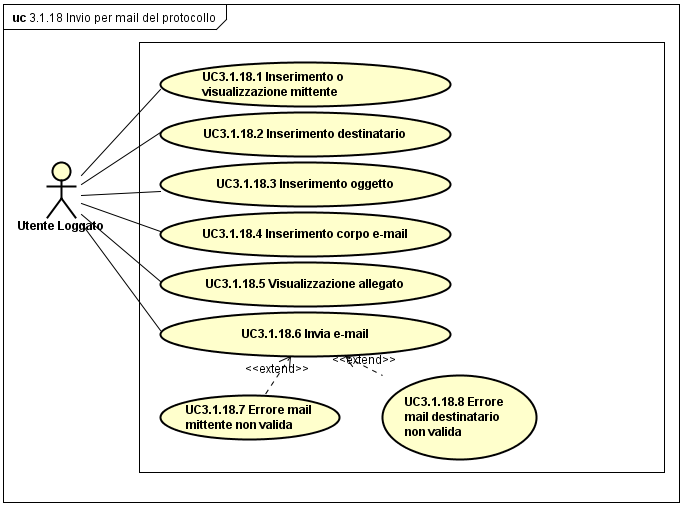
\includegraphics[width = 15cm]{immagini/UseCase/inviomail.png}
        \caption{UC3.1.18 Invio per mail del protocollo}
    \end{figure}
    
    \textbf{Attori primari:} Utente loggato.
    \\ 
    \\
    \textbf{Descrizione:} L'utente facendo \textit{click} sul tasto "Invia" citato in \hyperref[UC3.1]{UC3.1} accederà ad un form di compilazione ed invio di una e-mail.
    \\
    \\
    \textbf{Precondizione:} L'utente seleziona uno dei protocolli nella lista descritta in \hyperref[UC3]{UC3}.
    \\
    \\
    \textbf{Postcondizione:} Il sistema stampa a schermo il form di compilazione della mail.
    \\
    \\
    \textbf{Scenario principale:} L'utente deve inserire le seguenti informazioni per proseguire con l'invio della mail:
            \begin{itemize}
                \item mittente;
                \item destinatario;
                \item oggetto;
                \item corpo della e-mail;
                \item allegato;
                \item premere tasto "Invia" per inviare la mail.
            \end{itemize}
            

\subsubsection{UC4 Registrazione nuova configurazione}
    \label{UC4}
    \begin{figure}[!h] 
        \centering 
        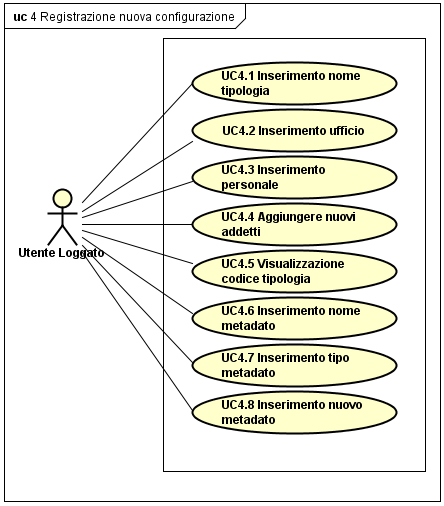
\includegraphics[width = 11cm]{immagini/UseCase/regnuovaconfig.png}
        \caption{UC4 Registrazione nuova configurazione}
    \end{figure}
    
    \textbf{Attori primari:} Utente loggato.
    \\ 
    \\
    \textbf{Descrizione:} L'utente è in grado di creare una nuova tipologia di documento.
    \\
    \\
    \textbf{Precondizione:} L'utente ha accesso all'apposita sezione del sito web.
    \\
    \\
    \textbf{Postcondizione:} Il sistema stampa a schermo il form di compilazione per registrare una nuova tipologia.
    \\
    \\
    \textbf{Scenario principale:} L'utente può:
            \begin{itemize}
                \item inserire nome tipologia;
                \item inserire nome ufficio;
                \item inserire personale dell'ufficio selezionato a cui attribuire l'elaborazione dei futuri protocolli;
                \item aggiungere nuovi addetti;
                \item visualizzare il codice attribuito alla tipologia in fase di creazione;
                \item inserire il nome di un metadato.
                \item inserire il tipo del metadato precedente;
                \item inserire un nuovo metadato.
            \end{itemize}
            
\subsubsection{UC4.4 Aggiungere nuovi addetti}
    \label{UC4.4}
    \textbf{Attori primari:} Utente loggato.
    \\
    \\
    \textbf{Descrizione:} L'utente premendo il tasto "Aggiungi" sito accanto alla selezione dell'ufficio e del personale aggiungerà una nuova riga dove poter selezionare un nuovo ufficio e dei nuovi addetti.
    \\
    \\
    \textbf{Precondizione:} L'utente seleziona "Aggiungi".
    \\
    \\
    \textbf{Postcondizione:} Il sistema stampa a video una nuova riga dove poter selezionare un nuovo ufficio e dei nuovi addetti.
    \\
    \\
    \textbf{Scenario principale:} L'attore può:
        \begin{itemize}
                \item inserire ufficio;
                \item inserire personale addetto;
            \end{itemize}
            
\subsubsection{UC4.8 Inserimento nuovo metadato}
    \label{UC4.8}
    \textbf{Attori primari:} Utente loggato.
    \\
    \\
    \textbf{Descrizione:} L'utente premendo il tasto "Aggiungi" sito accanto ai campi di inserimento di un metadato aggiungerà una nuova riga dove poter inserire il nome di un nuovo metadato e il tipo dello stesso.
    \\
    \\
    \textbf{Precondizione:} L'utente seleziona "Aggiungi".
    \\
    \\
    \textbf{Postcondizione:} Il sistema stampa a video una nuova riga dove poter inserire nome e tipo di un nuovo metadato.
    \\
    \\
    \textbf{Scenario principale:} L'attore può:
        \begin{itemize}
            \item inserire un nuovo metadato;
            \item inserire il tipo del nuovo metadato;
        \end{itemize}
        
\subsubsection{UC5 Visualizzazione lista delle configurazioni}
    \label{UC5}
    \textbf{Attori primari:} Utente loggato.
    \\
    \\
    \textbf{Descrizione:} L'utente visualizza una lista di tutti i protocolli che deve visionare.
    \\
    \\
    \textbf{Precondizione:} Il sistema pende dal database tutte le configurazioni esistenti.
    \\
    \\
    \textbf{Postcondizione:} Il sistema stampa a video tutte le configurazioni
    \\
    \\
    \textbf{Scenario principale:} L'attore può aprire la pagina dedicata alla visualizzazione delle informazioni riguardanti una singola tipologia di protocollo.
    
\subsubsection{UC5.1 Visualizzazione singola configurazione}
    \label{UC5.1}
    \begin{figure}[!h] 
        \centering 
        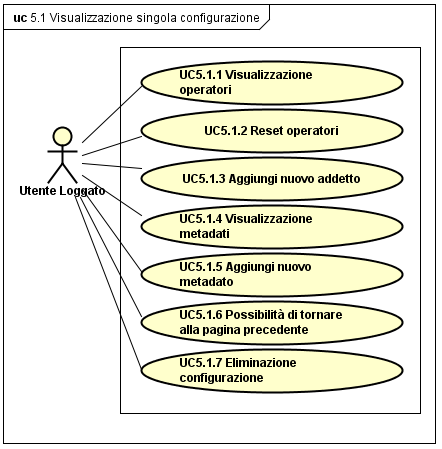
\includegraphics[width = 11cm]{immagini/UseCase/dettaglioconfig.png}
        \caption{UC5.1 Visualizzazione singola configurazione}
    \end{figure}
    
    \textbf{Attori primari:} Utente loggato.
    \\ 
    \\
    \textbf{Descrizione:} L'utente può visualizzare, modificare o eliminare le informazioni relative ad una tipologia.
    \\
    \\
    \textbf{Precondizione:} L'utente ha accesso all'apposita sezione del sito web.
    \\
    \\
    \textbf{Postcondizione:} Il sistema stampa a schermo le informazioni riguardanti una singola tipologia.
    \\
    \\
    \textbf{Scenario principale:} L'utente può:
            \begin{itemize}
                \item visualizzare gli operatori addetti;
                \item resettare la configurazione degli operatori;
                \item aggiungere un nuovo addetto
                \item visualizzare i metadati;
                \item aggiungere un nuovo metadato;
                \item tornare alla pagina precedente;
                \item eliminare una configurazione.
            \end{itemize}
%***************************************************************
\newpage
\subsection{Requisiti}

\subsubsection{Classificazione dei requisiti}
Ogni requisito sarà rappresentato con il seguente formalismo:
\begin{center}
    \textbf{R[Tipo][Utilità][Codice]}
\end{center}
dove:
\begin{itemize}
	\item
	\textbf{Tipo}: indica se il requisito è di tipo
	\begin{itemize}
	    \item \textbf{F}: indica un requisito di funzionale;
	    \item \textbf{Q}: indica un requisito di qualitativo;
	    \item \textbf{V}: indica un requisito di vincolo.
	\end{itemize}
	\item
	\textbf{Utilità}: può assumere i seguenti valori
	\begin{itemize}
	    \item \textbf{O (obbligatorio)}: questi requisiti dovranno necessariamente essere soddisfatti, in quanto di importanza fondamentale per la riuscita del progetto;
	    \item \textbf{D (desiderabile)}: questi requisiti non sono ritenuti fondamentali per la riuscita del progetto, tuttavia un loro soddisfacimento è percepito come desiderabile;
	    \item \textbf{F (facoltativo)}: il soddisfacimento di questi requisiti risulta del tutto facoltativo.
	\end{itemize}
	\item
	\textbf{Codice}: deve identificare in modo univoco ogni requisito. Per le gerarchie di requisiti, questo codice è nel formato [Codice padre].[Codice figlio].
\end{itemize}

\subsubsection{Requisiti funzionali}
Di seguito si riporta la tabella contenente tutti i requisiti funzionali individuati, comprensiva di descrizione del requisito, tracciamento dell'UC fonte dal quale esso ha origine (nel caso il requisito non sia stato descritto in un caso d'uso, verrà indicata come fonte "decisione interna") e stato di completamento raggiunto al termine dello stage (Completato/Non completato).
    \renewcommand{\arraystretch}{1.5}%
    \begin{longtable}{| p{3cm} | p{6cm} | p{3cm} | p{3cm} |}
        \caption[Requisiti Funzionali]{Requisiti Funzionali}
        \label{tabella:req0}
        \endlastfoot
        \hline
        \textbf{Requisito} & \textbf{Descrizione} & \textbf{fonte} & \textbf{Stato}\\
        \hline
        \endhead
        RFO1 & L'attore può accedere al sistema tramite login. & UC1 & Completato
        \\ \hline
        
        RFO1.1 & L'attore deve poter inserire il proprio codice utente. & UC1.1 & Completato
        \\ \hline
        
        RFO1.1.1 & L'attore deve poter visualizzare un messaggio d'errore qualora il codice utente sia sbagliato. & UC1.1.1 & Completato
        \\ \hline
        
        RFO1.2 & L'attore deve poter inserire la propria password & UC1.2 & Completato
        \\ \hline
        
        RFO1.2.1 & L'attore deve poter visualizzare un messaggio d'errore qualora la password sia sbagliata. & UC1.2.1 & Completato
        \\ \hline
        
        RFO2 & Deve essere possibile protocollare un documento & UC2 & Completato
        \\ \hline
        
        RFD1 & Deve essere possibile selezionare una tipologia di documento & UC2.1 & Completato
        \\ \hline
        
        RFO2.1 & Deve essere possibile selezionare la tipologia di un proprietario & UC2.2 & Completato
        \\ \hline
        
        RFO2.2 & Deve essere possibile inserire il nome del proprietario del protocollo & UC2.3 & Completato
        \\ \hline
        
        RFD2 & Deve essere possibile visualizzare i suggerimenti relativi al nome del proprietario & UC2.3 & Completato
        \\ \hline
        
        RFO2.3 & Deve essere possibile selezionare il registro di appartenenza & UC2.4 & Completato
        \\ \hline
        
        RFO2.4 & Al cambiare del registro di appartenenza deve essere stampato il rispettivo codice & UC2.4 e UC2.7 & Completato
        \\ \hline
        
        RFO2.5 & Deve essere possibile caricare un file & UC2.5 & Completato
        \\ \hline
        
        RFD3 & Deve essere possibile visualizzare il nome del file una volta caricato un documento & UC2.6 & Completato
        \\ \hline
        
        RFO2.6 & Deve essere possibile visualizzare il codice seriale univoco & UC2.7 & Completato
        \\ \hline
        
        RFO2.7 & Deve essere possibile visualizzare la data per la registrazione del protocollo & UC2.8 & Completato
        \\ \hline
        
        RFO2.8 & Deve essere possibile visualizzare l'ora per la registrazione del protocollo & UC2.9 & Completato
        \\ \hline
        
        RFO2.9 & Deve essere possibile visualizzare il codice dell'operatore che sta eseguendo la registrazione del protocollo & UC2.10 & Completato
        \\ \hline
        
        RFO2.10 & Deve essere possibile visualizzare un codice barcode univoco per il protocollo & UC2.11 & Completato
        \\ \hline
        
        RFO2.11 & Deve essere possibile modificare il barcode proposto dal sistema & UC2.12 & Completato
        \\ \hline
        
        RFD4 & Deve essere possibile inserire delle note & UC2.13 & Completato
        \\ \hline
        
        RFO2.12 & Deve essere possibile salvare il protocollo in inserimento & UC2.14 & Completato
        \\ \hline
        
        RFD5 & Deve essere possibile tornare indietro mediante bottone senza salvare il protocollo in elaborazione & UC2.15 & Completato
        \\ \hline
        
        RFO2.13 & Deve essere possibile inserire un nuovo contatto come proprietario del protocollo & UC2.16 & Completato
        \\ \hline
        
        RFO2.13.1 & Deve essere possibile inserire nome e cognome di un nuovo contatto & UC2.16.1 & Completato
        \\ \hline
        
        RFO2.13.2 & Deve essere possibile inserire un numero di telefono del nuovo contatto & UC2.16.2 & Completato
        \\ \hline
        
        RFO2.13.3 & Deve essere possibile inserire una e-mail del nuovo contatto & UC2.16.3 & Completato
        \\ \hline
        
        RFO2.13.4 & Deve essere possibile inserire la città di provenienza del nuovo contatto & UC2.16.4 & Completato
        \\ \hline
        
        RFO2.13.5 & Deve essere possibile inserire l'indirizzo del nuovo contatto & UC2.16.5 & Completato
        \\ \hline
        
        RFO2.13.6 & Deve essere possibile inserire il CAP del nuovo contatto & UC2.16.6 & Completato
        \\ \hline
        
        RFO2.13.7 & Deve essere possibile inserire la provincia del nuovo contatto & UC2.16.7 & Completato
        \\ \hline
        
        RFO3 & L'attore, in base ai suoi permessi, dovrà visualizzare la lista dei protocolli & UC3 & Completato
        \\ \hline
        
        RFO3.1 & Deve essere possibile visualizzare il singolo protocollo & UC3.1 & Completato
        \\ \hline
        
        RFO3.1.1 & Deve essere possibile visualizzare la tipologia di protocollo & UC3.1.1 & Completato
        \\ \hline
        
        RFO3.1.2 & Deve essere possibile visualizzare il registro di appartenenza del protocollo & UC3.1.2 & Completato
        \\ \hline
        
        RFO3.1.3 & Deve essere possibile visualizzare il codice seriale del protocollo & UC3.1.3 & Completato
        \\ \hline
        
        RFO3.1.4 & Deve essere possibile visualizzare il proprietario del protocollo & UC3.1.4 & Completato
        \\ \hline
        
        RFO3.1.5 & Deve essere possibile visualizzare il barcode assegnato al protocollo & UC3.1.5 & Completato
        \\ \hline
        
        RFO3.1.6 & Deve essere possibile visualizzare il nome del file allegato al protocollo & UC3.1.6 & Completato
        \\ \hline
        
        RFO3.1.7 & Deve essere possibile visualizzare l'operatore che ha provveduto alla registrazione del protocollo & UC3.1.7 & Completato
        \\ \hline
        
        RFO3.1.8 & Deve essere possibile visualizzare la data e l'ora di registrazione del protocollo & UC3.1.8 & Completato
        \\ \hline
        
        RFO3.1.9 & Deve essere possibile visualizzare i metadati del protocollo & UC3.1.9 & Completato
        \\ \hline
        
        RFO3.1.10 & Deve essere possibile visualizzare gli addetti all'elaborazione del protocollo & UC3.1.10 & Completato
        \\ \hline
        
        RFO3.1.11 \label{RFO3.1.11} & Deve essere possibile visualizzare lo storico e i commenti riguardanti il protocollo & UC3.1.11 & Completato
        \\ \hline
        
        RFO3.1.12 & Deve essere possibile inserire nuovi commenti riguardanti il protocollo & UC3.1.12 & Completato
        \\ \hline
        
        RFO3.1.13 & Deve essere possibile visualizzare le note relative al protocollo & UC3.1.13 & Completato
        \\ \hline
        
        RFF1 & Deve essere possibile visualizzare il flusso del protocollo & UC3.1.14 &  Non completato
        \\ \hline
        
        RFO3.1.14 & Deve essere possibile visualizzare l'anteprima del documento allegato al protocollo & UC3.1.15 & Completato
        \\ \hline
        
        RFO3.1.15 & Deve essere possibile scaricare il documento allegato al protocollo & UC3.1.16 & Completato
        \\ \hline
        
        RFO3.1.16 & Deve essere possibile per l'attore marcare come visualizzato il protocollo a lui assegnato & UC3.1.17 & Completato
        \\ \hline
        
        RFO3.1.17 & Deve essere possibile inviare per mail il protocollo & UC3.1.18 & Completato
        \\ \hline
        
        RFO3.1.17.1 & Deve essere possibile inserire o visualizzare il mittente & UC3.1.17.1 & Completato
        \\ \hline
        
        RFO3.1.17.2 & Deve essere possibile inserire il destinatario & UC3.1.17.2 & Completato
        \\ \hline
        
        RFO3.1.17.3 & Deve essere possibile inserire l'oggetto & UC3.1.17.3 & Completato
        \\ \hline
        
        RFO3.1.17.4 & Deve essere possibile inserire il testo della mail & UC3.1.17.4 & Completato
        \\ \hline
        
        RFO3.1.17.5 & Deve essere possibile visualizzare l'allegato caricato automaticamente come tale & UC3.1.17.5 & Completato
        \\ \hline
        
        RFO3.1.17.6 & Deve essere possibile inviare la mail& UC3.1.17.6 & Completato
        \\ \hline
        
        RFO3.1.17.7 & Deve essere possibile visualizzare un errore se l'indirizzo del mittente non è valido & UC3.1.17.7 & Completato
        \\ \hline
        
        RFO3.1.17.8 & Deve essere possibile visualizzare un errore se l'indirizzo del destinatario non è valido & UC3.1.17.8 & Completato
        \\ \hline
        
        RFO4 & Deve essere possibile registrare una nuova configurazione & UC4 & Completato
        \\ \hline
        
        RFO4.1 & Deve essere possibile inserire in nome della nuova tipologia & UC4.1 & Completato
        \\ \hline
        
        RFO4.2 & Deve essere possibile inserire un ufficio addetto all'elaborazione della suddetta tipologia & UC4.2 & Completato
        \\ \hline
        
        RFO4.3 & Deve essere possibile inserire il personale dell'ufficio selezionato & UC4.3 & Completato
        \\ \hline
        
        RFO4.3.1 & Deve essere possibile selezionare tutto il personale dell'ufficio & UC4.3 & Completato
        \\ \hline
        
        RFO4.3.2 & Deve essere possibile selezionare parte del personale dell'ufficio selezionato & UC4.3 & Completato
        \\ \hline
        
        RFO4.4 & Deve essere possibile aggingere una nuova composizione ufficio e personale & UC4.4 & Completato
        \\ \hline
        
        RFO4.4.1 & Deve essere possibile inserire un ufficio addetto all'elaborazione della suddetta tipologia & UC4.4.1 & Completato
        \\ \hline
        
        RFO4.4.2 & Deve essere possibile possibile inserire il personale dell'ufficio selezionato & UC4.4.2 & Completato
        \\ \hline
        
        RFO4.4.2.1 & Deve essere possibile selezionare tutto il personale dell'ufficio & UC4.3 & Completato
        \\ \hline
        
        RFO4.4.2.2 & Deve essere possibile selezionare parte del personale dell'ufficio selezionato & UC4.3 & Completato
        \\ \hline
        
        RFO4.5 & Deve essere possibile visualizzare il codice assegnato alla nuova configurazione & UC4.5 & Completato
        \\ \hline
        
        RFO4.6 & Deve essere possibile inserire il nome del metadato della nuova tipologia & UC4.6 & Completato
        \\ \hline
        
        RFO4.7 & Deve essere possibile inserire il tipo di metadato della nuova tipologia & UC4.7 & Completato
        \\ \hline
        
        RFO4.8 & Deve essere possibile inserire un nuovo metadato alla configurazione & UC4.8 & Completato
        \\ \hline
        
        RFO4.8.1 & Deve essere possibile inserire il nome del metadato della nuova tipologia & UC4.8.1 & Completato
        \\ \hline
        
        RFO4.8.2 & Deve essere possibile inserire il tipo di metadato della nuova tipologia & UC4.8.2 & Completato
        \\ \hline
        
        RFO5 & Deve essere possibile visualizzare la lista delle configurazioni & UC5 & Completato
        \\ \hline
        
        RFO5.1 & Deve essere possibile visualizzare la lista degli operatori addetti e i rispettivi uffici & UC5.1.1 & Completato
        \\ \hline
        
        RFO5.2 & Deve essere possibile resettare la configurazione degli operatori & UC5.1.2 & Completato
        \\ \hline
        
        RFO5.3 & Deve essere possibile aggiungere una nuova configurazione ufficio personale & UC5.1.3 & Completato
        \\ \hline
        
        RFO5.4 & Deve essere possibile visualizzare la lista dei metadati & UC5.1.4 & Completato
        \\ \hline
        
        RFO5.5 & Deve essere possibile aggiungere un nuovo metadato & UC5.1.5 & Completato
        \\ \hline
        
        RFO5.6 & Deve essere possibile tornare indietro senza salvare le modifiche alla configurazione & UC5.1.6 & Completato
        \\ \hline
        
        RFO5.7 & Deve essere possibile eliminare una configurazione qualora non ci siano documenti collegati alla suddetta & UC5.1.7 & Completato
        \\ \hline
        
        RFO6 \label{RFO6} & Deve essere possibile ricercare un protocollo mediante scanner di barcode & UC6 & Completato
        \\ \hline
        
        RFO7 & visualizzare e utilizzare la lista di filtri per la dashboard & UC7 & Completato
        \\ \hline
        
        RFF2 & Deve essere possibile visualizzare il ticket promemoria che ricorda all'utente quanti protocolli sono ancora da visionare  & UC8 & Completato
        \\ \hline
    \end{longtable}
\newpage

\subsubsection{Requisiti di vincolo}
    Di seguito si riporta la tabella contenente tutti i requisiti di vincolo individuati, comprensiva di descrizione del requisito e stato di completamento raggiunto al termine dello stage (Completato/Non completato).
    \renewcommand{\arraystretch}{1.5}%
    \begin{longtable}{| p{3cm} | p{9cm} | p{3cm} |}
        \caption[Requisiti di Vincolo]{Requisiti di Vincolo}
        \label{tabella:req0}
        \endlastfoot
        \hline
        \textbf{Requisito} & \textbf{Descrizione} & \textbf{Stato}\\
        \hline
        \endhead
        RVO1 & La pagina web deve funzionare correttamente su browser Google Chrome dalla versione 49 & Completato 
        \\ \hline
        
        RVO2 & La pagina web deve funzionare correttamente su browser Firefox dalla versione 5 & Completato 
        \\ \hline
        
        RVO3 & La pagina web deve funzionare correttamente su browser Microsoft Edge dalla versione 15 & Completato
        \\ \hline
        
        RVO4 & La pagina web deve funzionare correttamente su browser Safari dalla versione 11 & Completato 
        \\ \hline
    \end{longtable}

\subsubsection{Requisiti di qualità}
    Di seguito si riporta la tabella contenente tutti i requisiti di qualità individuati, comprensiva di descrizione del requisito e stato di completamento raggiunto al termine dello stage (Completato/Non completato).
    \renewcommand{\arraystretch}{1.5}%
    \begin{longtable}{| p{3cm} | p{9cm} | p{3cm} |}
        \caption[Requisiti di Vincolo]{Requisiti di Vincolo}
        \label{tabella:req0}
        \endlastfoot
        \hline
        \textbf{Requisito} & \textbf{Descrizione} & \textbf{Stato}\\
        \hline
        \endhead
        RQO1 & L'interfaccia utente deve essere sviluppata in lingua italiana & Completo
        \\ \hline
        
        RQO2 & Il processo di sviluppo del progetto deve attenersi ai principi qualitativi dell'azienda & Completato
        \\ \hline
        
        RQO3 & Il processo di sviluppo del progetto deve attenersi ai principi qualitativi dell'azienda & Completato
        \\ \hline
        
        RQO4 &  Lo sviluppo del progetto deve avvenire nei tempi previsti dal piano di lavoro & Completato
        \\ \hline
        
        RQD1 &  Deve essere fornita documentazione relativa all'analisi dei requisiti, mockup e struttura del software & Completato
        \\ \hline
    \end{longtable}
    \newpage
\subsubsection{Riepilogo dei requisiti}
    \normalsize
    \renewcommand{\arraystretch}{1.5}%
    \begin{longtable}{| p{3cm} | c | c | c || c |}
        \caption[Riepilogo Requisiti]{Riepilogo Requisiti}
        \label{tabella:riepilogorequi}
        \endlastfoot
        \hline
        \textbf{Tipo} & \textbf{Obbligatorio} & \textbf{Desiderabile} & \textbf{Facoltativo} & Totale\\
        \hline
        Funzionali & 80 & 4 & 2 & 86\\ \hline
        Vincolo & 4 & 0 & 0 & 4\\ \hline
        Qualità & 4 & 1 & 0 & 5\\ \hline \hline
        Totale & 88 & 5 & 2 & 95\\ \hline
    \end{longtable}

%**************************************************************


\section{Soluzione proposta}
In questo paragrafo verrà riportata la soluzione ideata da me e dal tutor aziendale per far fronte alle esigenze dell'azienda proponente.
\\
Le immagini a sostegno di quanto descritto, realizzate con il software gratuito \emph{MockFlow}\glsfirstoccur, fanno parte di un documento da me creato con lo scopo di presentare un possibile layout finale all'azienda proponente. Il documento è stato molto apprezzato sia dal tutor che dagli utilizzatori finali.
\subsection{Mockup}

\subsubsection{Gestione livelli di accesso e autorizzazioni}
Gli operatori avranno possibilità di accesso diverse a seconda dei ruoli svolti, suddividendo questi in:
    \begin{itemize}
        \item \textbf{Utente base:} inserisce protocolli e gestisce solo quelli da lui creati o a lui assegnati;
        
        \item \textbf{Amministratore:} inserisce protocolli, gestisce tutti quelli creati da ogni utente e gestisce le configurazioni delle tipologie e dei flussi dei protocolli. 
    \end{itemize}

\subsubsection{Registrazione di un protocollo}
I protocolli sono suddivisi in tre registri: Spediti - Ricevuti - Interni.
\\
Ogni registrazione ha un suo progressivo di inserimento. Questo è composto dalla prima lettera che fa riferimento al registro selezionato e i restanti numeri indicano il successivo all'ultimo inserimento per quel determinato registro.
\\
Durante la registrazione verrà reso disponibile un campo "barcode documento" per poter leggere il barcode che identifica il documento in ingresso ed associarlo ad un'eventuale scansione automatica del file.
\\
È previsto l'upload di un file a corredo dei dati di registrazione.

\begin{figure}[!h] 
    \centering 
    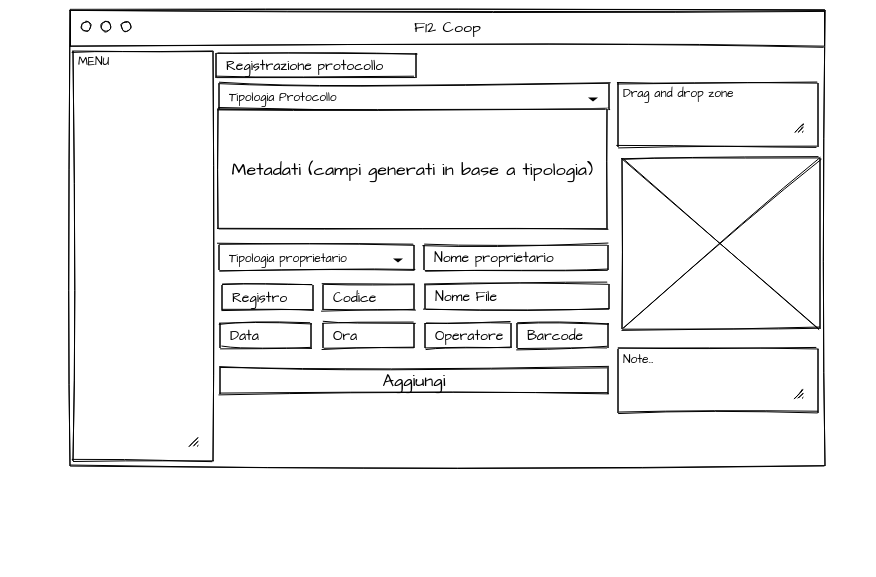
\includegraphics[width=1\columnwidth]{immagini/mockup/Registrazioneprotocollo.png} 
    \caption{Mockup - Registrazione Protocollo}
\end{figure}
\newpage

In base alla tipologia del protocollo selezionata verranno generati dei campi "metadati" con lo scopo di arricchire di informazioni il protocollo per una più facile consultazione.
\\ 
La scelta del tipo di proprietario a cui intestare il protocollo prevede la voce "nuovo contatto" che se selezionata farà comparire un form di registrazione.
\\
Una volta premuto il tasto "Aggiungi" i dati inseriti verranno salvati nelle rispettive tabelle del \textit{database}, compreso il nuovo contatto inserito.
\\
La tipologia del protocollo e i metadati saranno configurabili dall'apposito pannello descritto in "Configurazione tipologia documento".

\subsubsection{Dashboard generale}
Nella dashboard, in base all'utente che ha eseguito l'accesso, si potrà trovare l'elenco in forma tabellare di tutti i protocolli.
\\
Nell'intestazione della pagina, per facilitare l'operatore nella ricerca di specifici protocolli, saranno presenti: i campi filtrabili, un campo input che con il focus su di esso permette di filtrare i protocolli mediante scanner di barcode e un ticket promemoria che ricorda all'utente quanti protocolli deve ancora visionare.
\begin{figure}[!h] 
    \centering 
    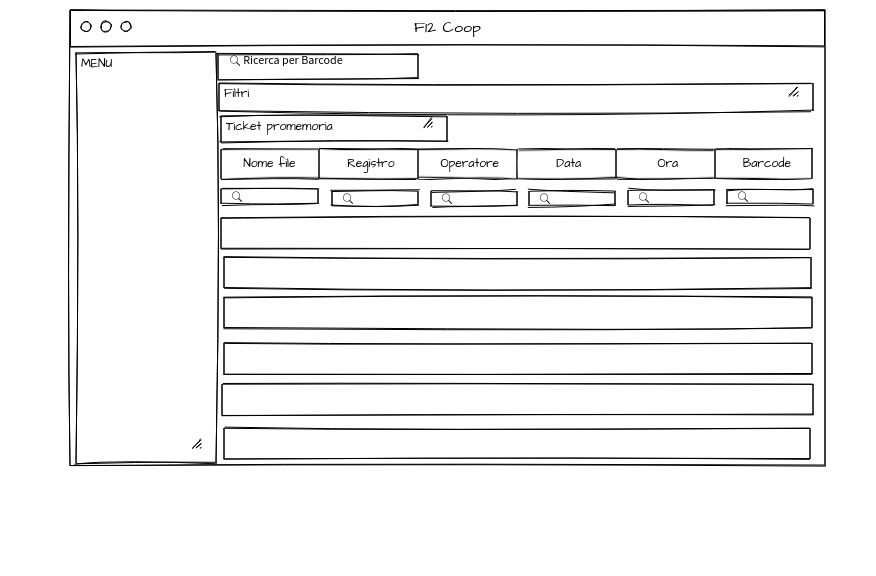
\includegraphics[width=1\columnwidth]{immagini/mockup/Dashboard.png}
    \caption{Mockup - Dashboard}
\end{figure}
\newpage

\subsubsection{Dettaglio protocollo}
Selezionando uno qualsiasi dei protocolli dalla lista precedentemente citata si aprirà la seguente pagina.
\begin{figure}[!h] 
    \centering 
    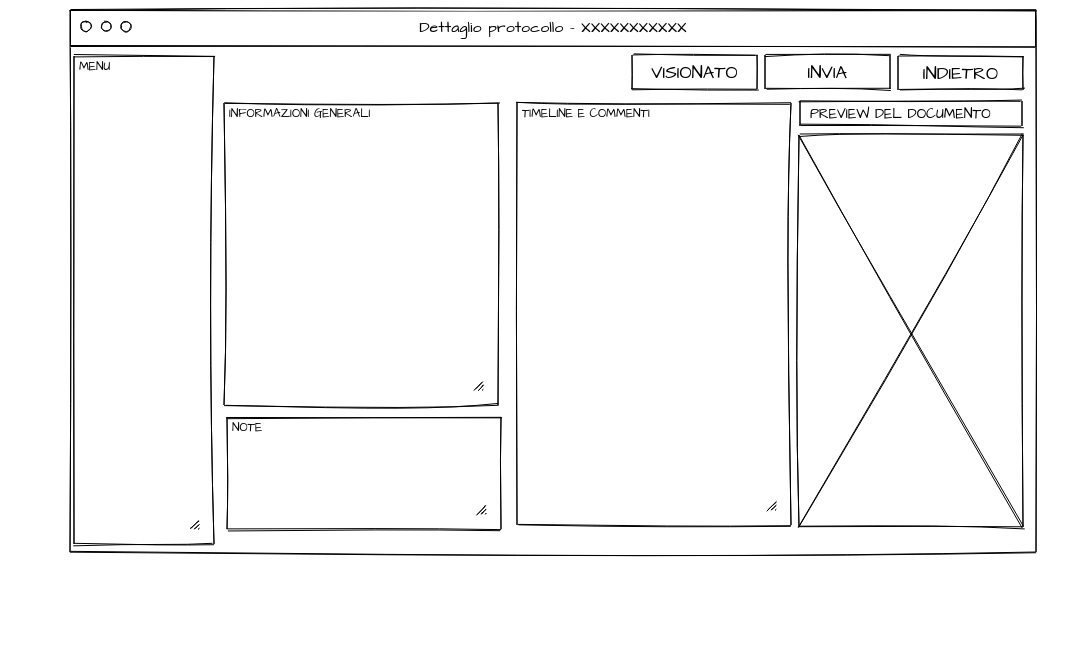
\includegraphics[width=1\columnwidth]{immagini/mockup/Editpage.png}
    \caption{Mockup - Pagina dettaglio protocollo}
\end{figure}
\\
Tra le informazioni generali, in base alla tipologia di protocollo selezionata, sarà presente la lista degli operatori addetti all'elaborazione del documento.
\\
L'utente premendo il bottone "VISIONATO" farà comparire accanto al proprio nome nella lista una spunta verde. Una volta esaminato da tutti gli operatori il protocollo sarà marcato come "visionato" e se il flusso assegnatogli lo richiede esso proseguirà con il task successivo.
\\
Premendo il tasto "INVIA" l'utente verrà rimandato ad una schermata dove è possibile compilare un form per l'invio via mail. 
\\
In fase di preparazione della e-mail verranno proposti gli indirizzi dell'intestatario del protocollo e gli indirizzi del personale interno.
\\
Nel corpo della e-mail verrà presentata una bozza di testo dove vengono riportati tutti i dati raccolti in fase di registrazione.
\\
Tra gli allegati sarà già presente il documento corrispondente al protocollo che si vuole inviare.
\\
In figura (figura 2.4), la sezione marcata come "TIMELINE E COMMENTI" ha lo scopo di far fronte all'esigenza della proponente di avere sempre visibile lo storico del protocollo. È stata inoltre aggiunta la possibilità di scrivere commenti rendendo questa sezione una vera e propria chat organizzativa.

\subsubsection{Configurazione tipologia protocollo}
Tra le voci di menù nella sezione protocolli è possibile accedere alla schermata di configurazione delle tipologie.
\begin{figure}[!h] 
    \centering 
    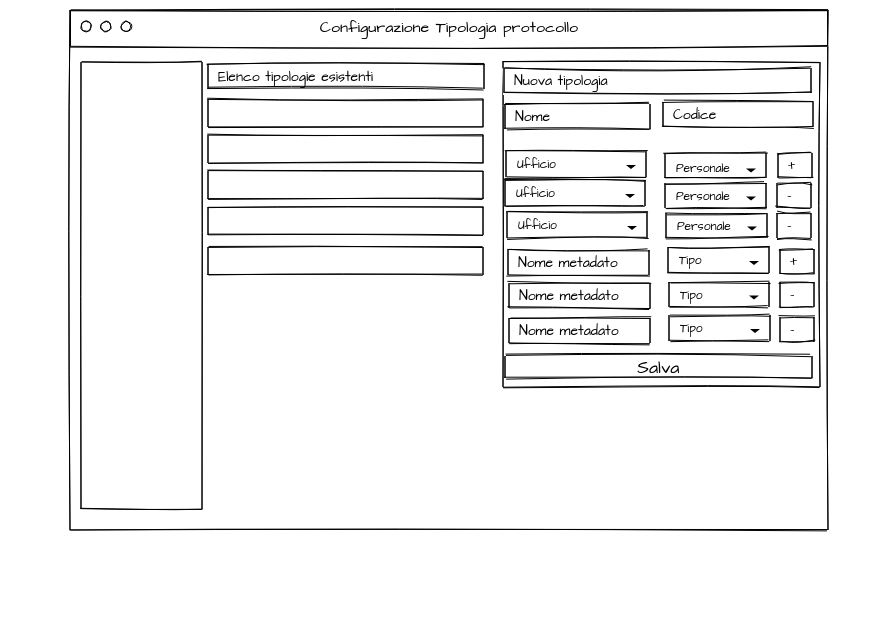
\includegraphics[width=1\columnwidth]{immagini/mockup/configtipo.png}
    \caption{Mockup - Pagina di configurazione delle tipologie}
\end{figure}
\\
La seguente maschera è pensata per far fronte all'esigenza di configurare un protocollo in base alla sua tipologia e quindi arricchirlo di informazioni utili alla facile consultazione e archiviazione. Sarà quindi possibile visionare l'elenco di tutte le tipologie di protocolli create nella lista sulla sinistra e sulla destra un semplice form per la creazione di una nuova tipologia.
\\
Come detto in precedenza, creando una nuova tipologia sarà possibile assegnare il personale addetto all'elaborazione della suddetta e sarà possibile aggiungere campi metadato.

\subsubsection{Dettaglio configurazione tipologia protocollo}
Selezionando una qualsiasi delle tipologie dalla lista precedentemente citata si aprirà la seguente pagina.
\begin{figure}[!h] 
    \centering 
    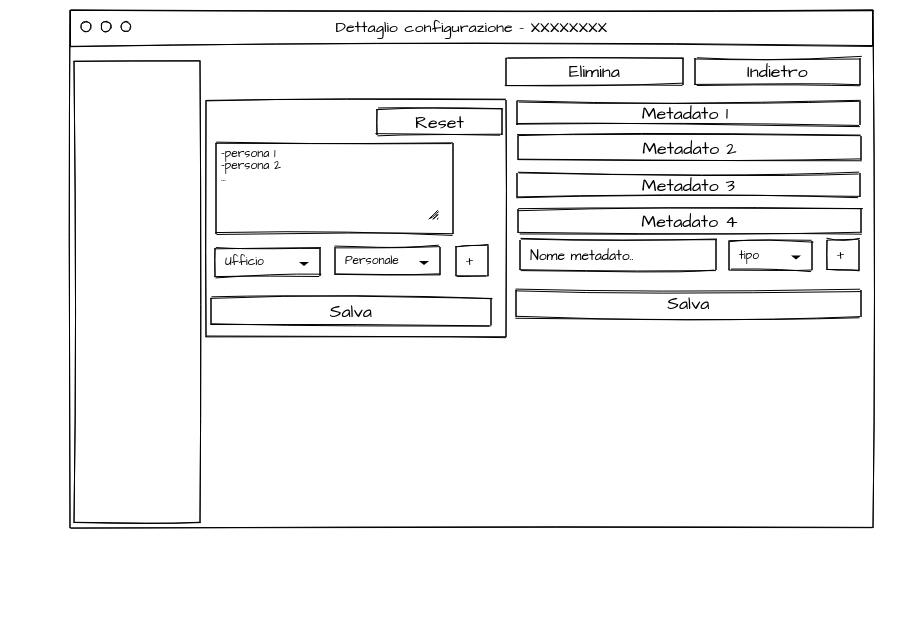
\includegraphics[width=1\columnwidth]{immagini/mockup/dettaglioconfig.png}
    \caption{Mockup - Pagina dettaglio configurazione tipologia}
\end{figure}
\\
Saranno visibili tutti i metadati e gli addetti precedentemente inseriti e sarà possibile aggiungerne di nuovi.\\
L'eliminazione di una configurazione sarà consentita solo nel caso in cui non ci saranno documenti associati alla configurazione in esame.
%**************************************************************
\newpage
\subsection{Struttura del software}
La struttura finale del software sarà la seguente.

\begin{figure}[!h] 
    \centering 
    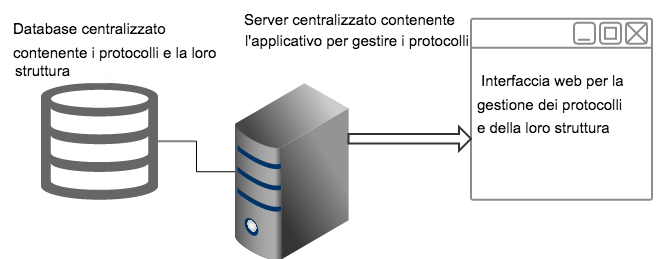
\includegraphics[width=1\columnwidth]{immagini/prodottofinito/strutturasoftware.png}
    \caption{Struttura del software}
\end{figure}

%**************************************************************
% !TEX encoding = UTF-8
% !TEX TS-program = pdflatex
% !TEX root = ../tesi.tex

%**************************************************************
\chapter{Protocollazione}
\label{cap:protocollazione}
%**************************************************************

\intro{Tale capitolo riporta una descrizione approfondita di cos'è un protocollo, come si deve registrare un protocollo e i possibili flussi applicativi che esso può percorrere}\\

%**************************************************************
\section{Definizione di protocollo}
La definizione di protocollo informatico, chiamato anche protocollo informatizzato, può essere tratta dal "Testo unico" in materia di documentazione amministrativa (DPR n. 445 del 28 dicembre 2000): "il legislatore ha individuato nel protocollo informatico quell'insieme di procedure informatizzate e di infrastrutture ICT (risorse di calcolo, apparati e reti di comunicazione) che le amministrazioni impiegano per la gestione documentale".
\\
\\
La protocollazione dei documenti non è intesa come mera operazione amministrativa, ma un vero e proprio procedimento amministrativo diffuso che mira alla dematerializzazione dei flussi documentali e a tutti i vantaggi che essa comporta.
Questi vantaggi, che riguardano principalmente la gestione del documento, sono:
\begin{itemize}
    \item \textbf{Flessibilità:} il documento prodotto in formato dematerializzato potrà essere corredato e completato con diverse tipologie di documenti;
    
    \item \textbf{Simulazione:} si potranno produrre infinite copie dello stesso documento conformi all'originale;
    
    \item \textbf{Conservazione:} il documento potrà essere conservato per un periodo di tempo lungo senza subire deterioramento;
    
    \item \textbf{Trasmissibilità:} il vantaggio del trasferimento dei documenti digitali è evidente;
    
    \item \textbf{Archiviazione:} grazie a determinati strumenti informatici, si può arrivare a un sistema di archiviazione e di correlazioni tra documenti che rende il loro accesso più semplice e rapido.
\end{itemize}
Un documento protocollato, dal momento della protocollazione stessa, verrà tratto sotto il profilo giuridico e gestionale.
\\
Si può quindi affermare che il protocollo è il punto di snodo di tutta la corrispondenza in entrata e in uscita di un'azienda ed è la chiave di accesso all'informazione e alla documentazione.
%**************************************************************
\section{Registrazione di un protocollo}
La registrazione di un protocollo attesta che un determinato documento è stato prodotto (arrivato, spedito o interno) in una data determinata, ha funzione giuridico-probatoria e attesta l’esistenza all'interno dell'archivio di un determinato documento.
\\
Per questo motivo le informazioni minime previste da DPR 28 dicembre 2000, n. 445 - art. 56 sono:
\begin{itemize}
    \item un codice univoco di protocollo generato automaticamente dal sistema e registrato in forma non modificabile;
    
    \item data di registrazione di protocollo assegnata automaticamente dal sistema e registrata in forma non modificabile;
    
    \item mittente per i documenti ricevuti o, in alternativa, il destinatario o i destinatari per i documenti spediti, registrati in forma non modificabile;
    
    \item oggetto del documento, registrato in forma non modificabile;
    
    \item descrizione dei documenti allegati;
    
    \item data e protocollo del documento ricevuto, se disponibili;
    
    \item l’impronta del documento informatico, se trasmesso per via telematica, costituita dalla sequenza di simboli binari in grado di identificarne univocamente il contenuto, registrata in forma non modificabile.
\end{itemize}

%**************************************************************
\section{Flusso applicativo di un protocollo}
A differenza degli “iter procedurali”, che prevedono passaggi lineari al verificarsi di una determinata condizione, il flusso digitale (\emph{workflow}\glsfirstoccur) si articola in percorsi intelligenti, definiti tenendo presente l’organigramma aziendale.
\\
Un flusso di questo tipo consente di controllare in tempo reale le fasi del ciclo esecutivo e di valutarne oggettivamente la validità, ridurre gli errori, migliorare la collaborazione e la qualità del servizio e ridurre i costi di gestione e di addestramento del personale. È possibile ridurre i costi di addestramento in quanto il software guida l'utente nei vari passaggi di gestione del protocollo.
\\
\\
Esempi di flussi documentale potrebbe essere i seguenti.
\begin{figure}[!h] 
    \centering 
    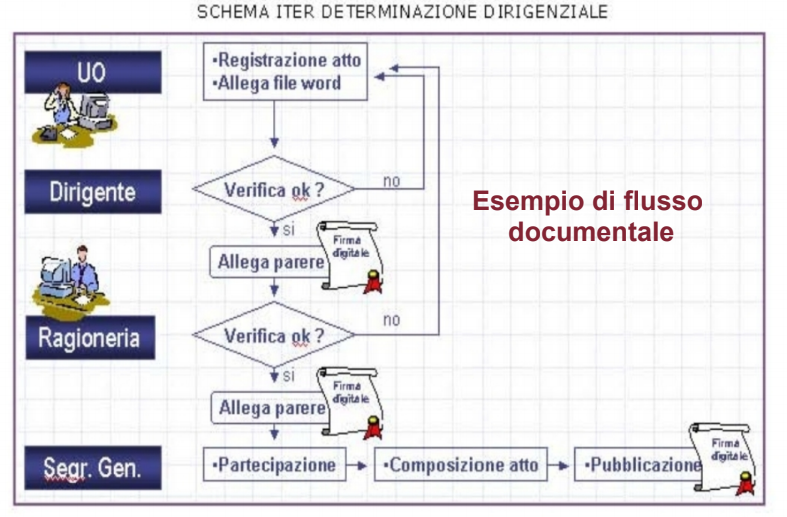
\includegraphics[width=1\columnwidth]{immagini/flussi/Flusso1.png} 
    \caption{Esempio di flusso documentale}
\end{figure}
\begin{figure}[!h] 
    \centering 
    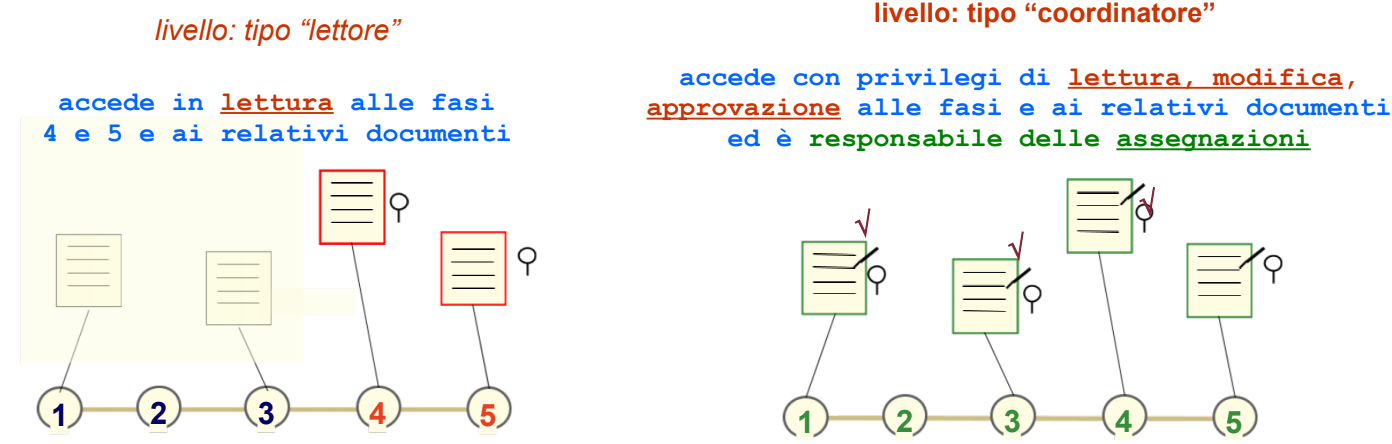
\includegraphics[width=1\columnwidth]{immagini/flussi/flusso2.png} 
    \caption{Esempio di flusso documentale}
\end{figure}
\newpage

Solo mediante il deposito di un documento elettronico in una base di dati alla
quale si attinge secondo necessità, con diverse autorizzazioni di
lettura/scrittura, è possibile gestire i flussi documentali.
\\
È quindi possibile affermare che ogni sistema di protocollazione a norma si appoggia su una piattaforma documentale.

% !TEX encoding = UTF-8
% !TEX TS-program = pdflatex
% !TEX root = ../tesi.tex

%**************************************************************
\chapter{Gestione documentale}
\label{cap:gestione-documentale}
%**************************************************************

\intro{Il seguente capitolo riporta una descrizione dettagliata del software F12 Documentale fornitomi per l'archiviazione dei documenti in upload durante la registrazione di un protocollo.\\
Nelle immagini esplicative i dati sensibili di aziende o persone sono oscurati per motivi di privacy.}\\

\section{F12 - Documentale}
Il software documentale sviluppato da Gestiware nasce per migliorare e potenziare il livello di integrazione fra F12 e una gestione documenale web esterna.

    \subsection{Tipologie di documenti}
    Di seguito le categorie di documenti che vengono gestite:
    \begin{itemize}
        \item documenti prodotti da F12 (flusso attivo);
        
        \item documenti da flusso passivo (flusso passivo);
        
        \item documenti tecnici o estemporanei collegati a varie entità di F12.
    \end{itemize}
    
    Ogni documento sarà associato ad un tipo di documento. Il tipo del documento identifica una classe di documenti (ad esempio le “fatture”) e quindi definisce lo schema di informazioni aggiuntive che hanno attinenza con i documenti così classificati. Queste informazioni di corredo verranno chiamati metadati. Ogni documento appartiene ad una ed una sola classe.
    \\
    \\
    È possibile creare una configurazione dove vengono definiti i tipi di documenti che vogliamo gestire (fattura, ddt,...,generico) e i metadati che vogliamo associare ad ogni tipo di documento. Per ogni metadato è possibile configurare il singolo campo di database dove il metadato può essere letto. Questo serve per poter estrarre o aggiornare i metadati di un documento automaticamente nel momento in cui questo viene caricato.
    \\
    \\
    Tutti i documenti di F12 avranno i seguenti metadati in comune:
    \begin{itemize}
        \item seriale;
        
        \item tipo\_documento;
        
        \item autore;
        
        \item data\_caricamento;
        
        \item data\_ultima\_modifica;
        
        \item barcode.
    \end{itemize}
    
    I documenti vengono identificati per mezzo di un seriale univoco che non permette la coesistenza, nel gestore documentale, di due documenti (semanticamente) distinti con lo stesso seriale. Ogni documento potrà avere anche un barcode associato.
    \\
    Inoltre può subire delle variazioni o essere modificato, questo comporta un aggiornamento della versione del documento. La nuova versione del documento ha lo stesso seriale ma ha incrementato il contatore della sua versione.
    
    \subsection{Flusso attivo}
    I documenti generati dal gestionale possono essere archiviati nel sistema documentale mediante due modalità:
    \begin{itemize}
        \item nel momento in cui F12 genera un nuovo documento, invoca una procedura del sistema documentale passandogli il file generato e i dati necessari all'archiviazione;
        
        \item la seconda modalità consiste in una procedura che elabora i file generati dalla coda di stampa e associa automaticamente il file all'entità corrispondente, basandosi sul nome del file oppure sull'xml associato al file contente i dati necessari all'archiviazione documentale.
    \end{itemize}
    
    \subsection{Flusso passivo}
    I documenti possono essere caricati manualmente attraverso l'interfaccia web presente sulle maschere di F12 oppure attraverso il portale web documentale.
    \\
    I documenti caricati tramite F12 sono collegati automaticamente all'entità di F12 in quanto il caricamento del file avviene sull'entità stessa.
    \\
    In caso di caricamento di file da portale web verranno richieste le informazioni necessarie al collegamento automatico del documento con l'entità di F12 (tipo entità, seriale, barcode ecc...).
    
    \subsection{Permessi su file e sicurezza}
    I permessi e le azioni che l'utente può effettuare sui file saranno ereditati dai permessi collegati ai gruppi di F12.
    \\
    È necessario aggiungere alla tabella di configurazione delle “tipologie dei documenti” un campo per settare il permesso corrispondete al gruppo per poter operare su quel tipo di documento.
    \\
    Ad esempio il gruppo amministrazione sarà associato ai documenti di tipo fattura.
    \\
    I file sono archiviati nel file system in forma criptata, senza estensione, di modo che siano leggibili solo attraverso il software documentale.

    \subsection{Gestione dei documenti}
    L'accesso al gestore documentale può essere effettuata sia lato web che lato client F12, e l'aggiunta di documenti alle entità di F12 potrà essere fatta da entrambi i lati.
        
        \subsubsection{Accesso documentale con F12}
        L'accesso all'interfaccia documentale su F12 avviene attraverso una maschera web caricata all'interno dell'entità per la quale si vuole abilitare il documentale e si potranno caricare documenti di tipologie abilitate per quel tipo di entità. 
        \\
        Si possono inoltre caricare anche documenti generici, tuttavia per questo tipo di documenti non sono definiti altri metadati oltre a quelli base.
        \begin{figure}[!h] 
            \centering 
            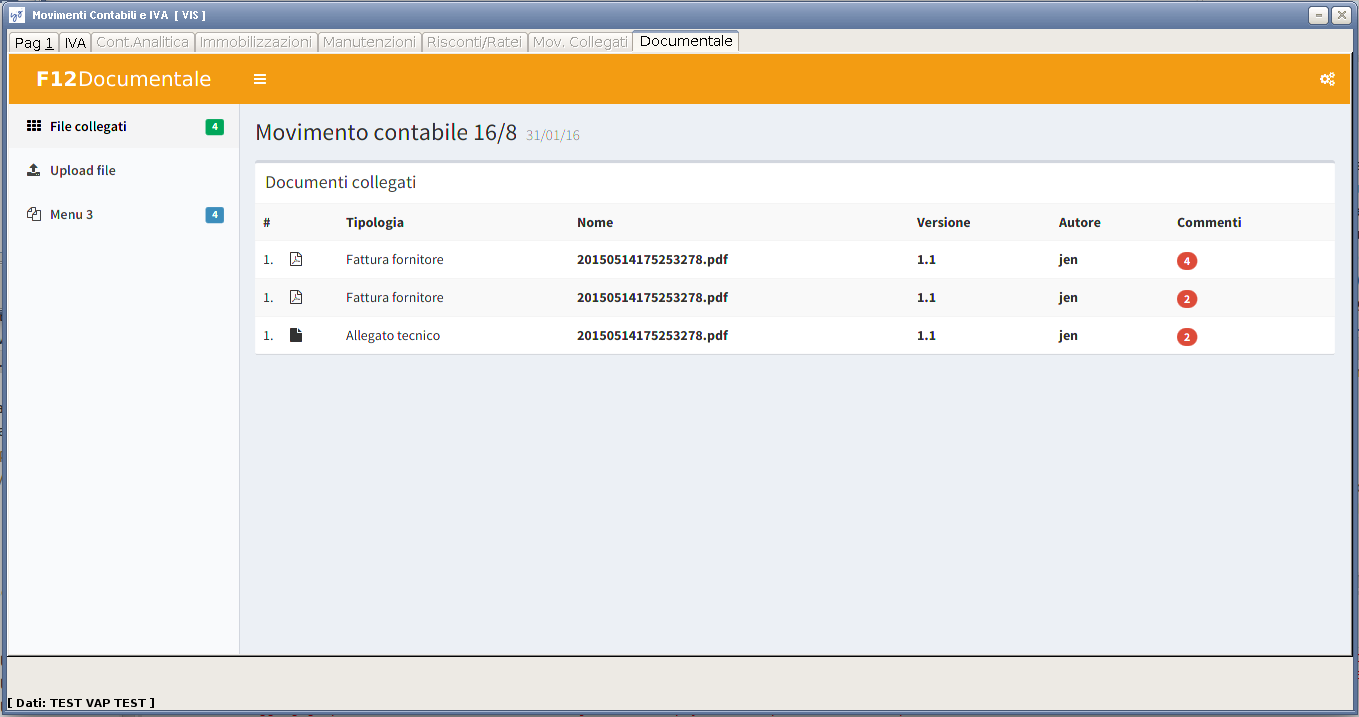
\includegraphics[width=1\columnwidth]{immagini/f12doc/1.png}
            \caption{Esempio di maschera documentale visibile per l'entità “movimento contabile 16/8”}
        \end{figure}
        \begin{figure}[!h] 
            \centering 
            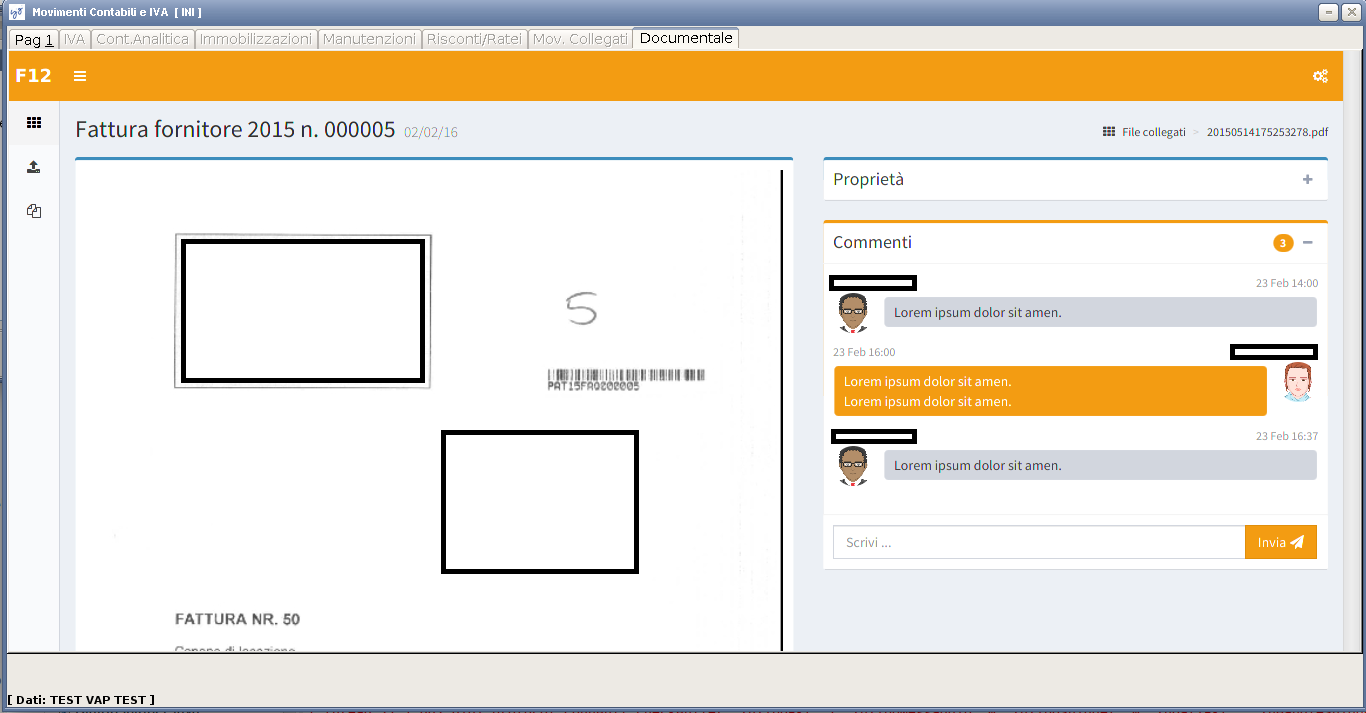
\includegraphics[width=1\columnwidth]{immagini/f12doc/2.png}
            \caption{Esempio di maschera di dettaglio di un documento 1}
        \end{figure}
        \begin{figure}[!h] 
            \centering 
            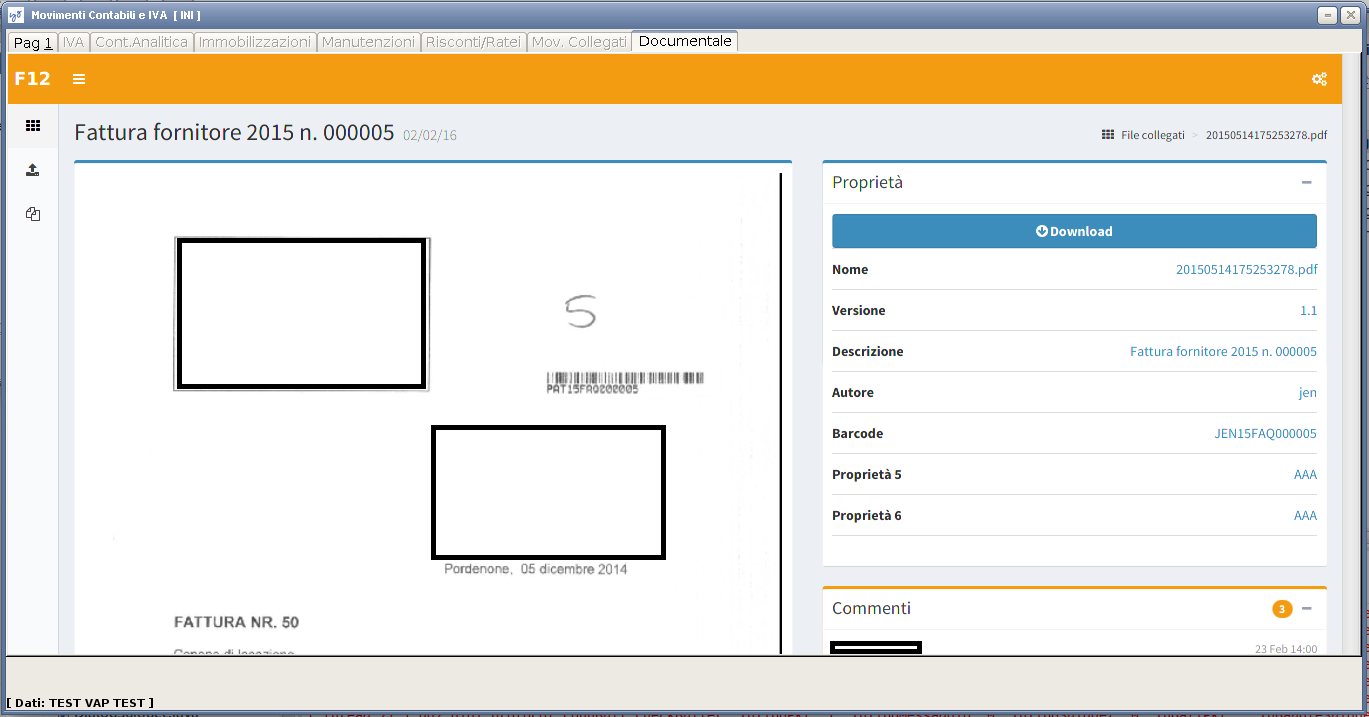
\includegraphics[width=1\columnwidth]{immagini/f12doc/3.png}
            \caption{Esempio di maschera di dettaglio di un documento 2}
        \end{figure}
        \newpage
        Attraverso questa maschera web si potranno:
        \begin{itemize}
            \item caricare documenti nuovi definendo preventivamente il tipo di documento che si sta caricando (Per aggiornare automaticamente i metadati);
            
            \item aggiungere, togliere, modificare metadati;
            
            \item caricare nuove versioni dello stesso documento;
            
            \item commentare i documenti.
        \end{itemize}
        È inoltre possibile ricercare e consultare i documenti su una maschera web caricata a parte.
        
        \subsubsection{Accesso documentale tramite Web}
        Sarà possibile accedere al documentale tramite interfaccia web.
        \\
        Attraverso essa si potranno:
        \begin{itemize}
            \item cercare documenti;
            
            \item sfogliare le directory della \textit{repository};
            
            \item consultare le anteprime dei documenti;
            
            \item scaricare i documenti;
            
            \item commentare  i documenti;
            
            \item aggiungere, togliere, modificare i metadati;
            
            \item gestire le tipologie di documenti e i metadati;
            
            \item caricare revisioni di un documento;
            
            \item caricare nuovi documenti attraverso un'apposita interfaccia (Si potranno stabilire delle condizioni attraverso le quali i nuovi documenti caricati saranno collegati automaticamente alle entità di F12).
        \end{itemize}
        \begin{figure}[!h] 
            \centering 
            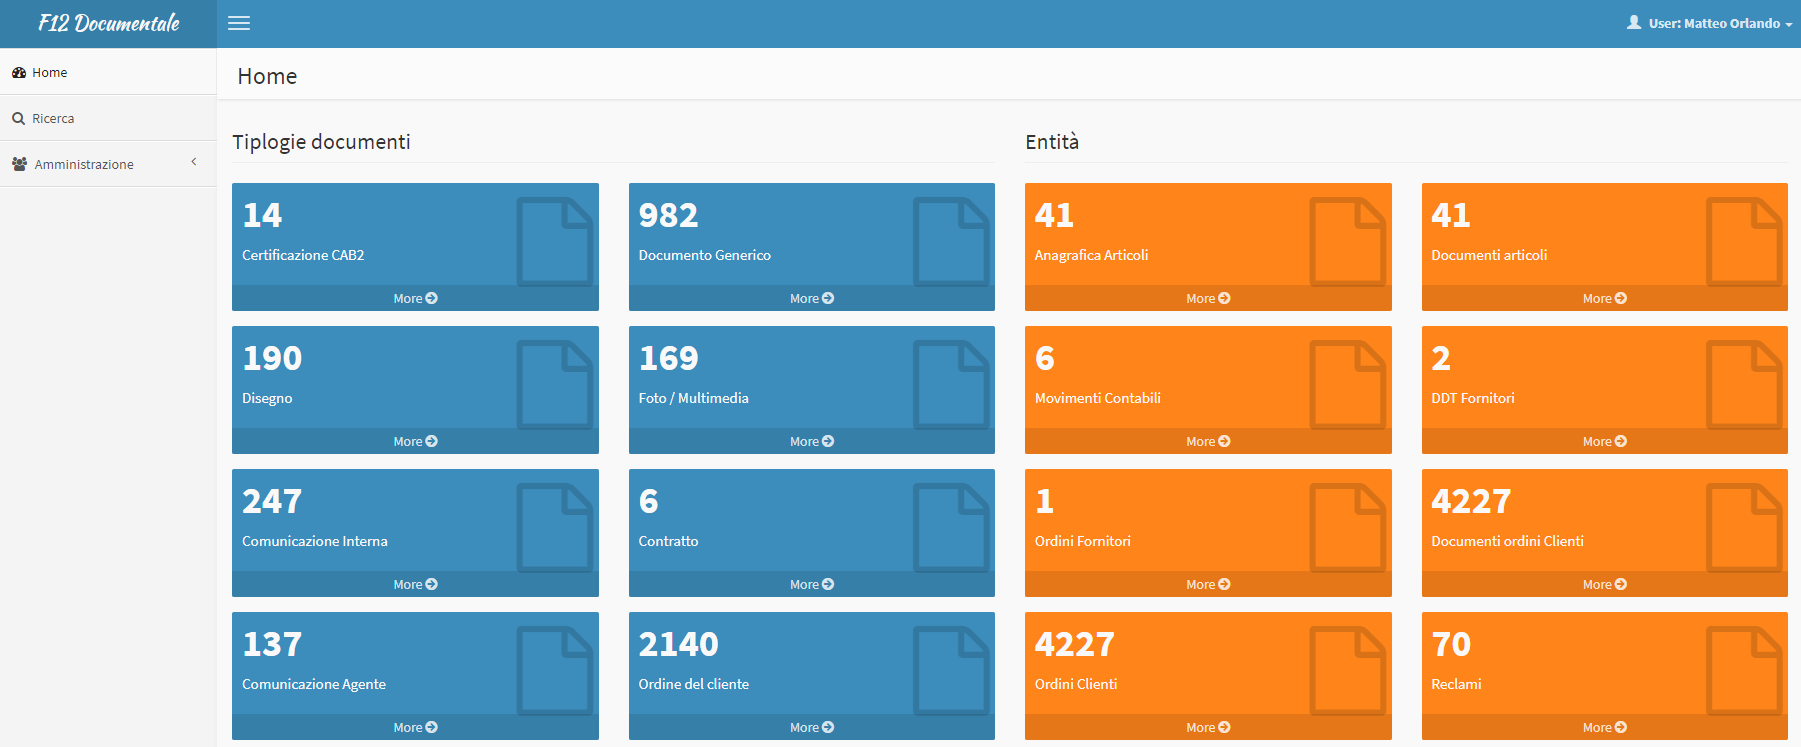
\includegraphics[width=1\columnwidth]{immagini/f12doc/4.png}
            \caption{Esempio di maschera documentale visibile per l'entità “movimento contabile 16/8”}
        \end{figure}
% !TEX encoding = UTF-8
% !TEX TS-program = pdflatex
% !TEX root = ../tesi.tex

%**************************************************************
\chapter{Progettazione e codifica}
\label{cap:progettazione-codifica}
%**************************************************************

%**************************************************************
\section{Tecnologie usate}
\label{sec:tecnologie-strumenti}

Per la realizzazione del progetto di stage è stato dedicato diverso tempo all'apprendimento delle tecnologie e linguaggi richiesti, di seguito elencati.

\subsection{Linguaggi di programmazione}

\subsubsection{PHP}
PHP (acronimo ricorsivo di "PHP: Hypertext Preprocessor") è un linguaggio di \textit{scripting} interpretato, originariamente concepito per la programmazione di pagine web dinamiche. L'interprete PHP è un software libero distribuito sotto la PHP License.
\\
Attualmente è principalmente utilizzato per sviluppare applicazioni web lato server, ma può essere usato anche per scrivere script a riga di comando o applicazioni \textit{stand-alone} con interfaccia grafica.
\\
\begin{figure}[!h] 
    \centering 
    
\includegraphics[width=4cm]{immagini/loghi/php.png}
    \caption{Logo PHP}
\end{figure}

\subsubsection{JavaScript}
JavaScript è un linguaggio di \textit{scripting} orientato agli oggetti e agli eventi, comunemente utilizzato nella programmazione Web lato \textit{client} per la creazione, in siti web e applicazioni web, di effetti dinamici interattivi tramite funzioni di script invocate da eventi innescati a loro volta in vari modi dall'utente sulla pagina web in uso.
\begin{figure}[!h] 
    \centering 
    
\includegraphics[height=3cm]{immagini/loghi/javascript.png}
    \caption{Logo JavaScript}
\end{figure}

\subsubsection{AJAX}
AJAX, acronimo di Asynchronous JavaScript and XML, è una tecnica di sviluppo software per la realizzazione di applicazioni web interattive (Rich Internet Application). Lo sviluppo di applicazioni HTML con AJAX si basa su uno scambio di dati in background fra web browser e server, che consente l'aggiornamento dinamico di una pagina web senza esplicito ricaricamento da parte dell'utente.
\begin{figure}[!h] 
    \centering 
    
\includegraphics[width=3cm]{immagini/loghi/ajax.png}
    \caption{Logo AJAX}
\end{figure}
AJAX è asincrono nel senso che i dati extra sono richiesti al server e caricati in background senza interferire con il comportamento della pagina esistente. Normalmente le funzioni richiamate sono scritte con il linguaggio JavaScript. Tuttavia, e a dispetto del nome, l'uso di JavaScript e di XML non è obbligatorio, come non è detto che le richieste di caricamento debbano essere necessariamente asincrone.

\subsubsection{HTML 5}
L'HTML5 è un linguaggio di \textit{markup} per la strutturazione delle pagine web, pubblicato come \textit{W3C Recommendation} da ottobre 2014.
\\
\begin{figure}[!h] 
    \centering 
    
\includegraphics[height=3cm]{immagini/loghi/html.png}
    \caption{Logo HTML5}
\end{figure}
\\
Gli obiettivi di HTML5 sono di migliorare il linguaggio con il supporto agli ultimi file multimediali ed altre \textit{features}; di mantenere il linguaggio sia leggibile dagli umani che consistente tra i vari dispositivi e browser, abbandonando la rigidità dell'XHTML, rimanendo retrocompatibile con i software più vecchi.


\subsubsection{CSS 3}
Il CSS (acronimo di Cascading Style Sheets), in informatica, è un linguaggio usato per definire la formattazione di documenti HTML, XHTML e XML ad esempio i siti web e relative pagine web. Le regole per comporre il CSS sono contenute in un insieme di direttive (Recommendations) emanate a partire dal 1996 dal W3C.
\\
\begin{figure}[!h] 
    \centering 
    
\includegraphics[height=3cm ]{immagini/loghi/css.png}
    \caption{Logo CSS3}
\end{figure}
\\
L'introduzione del CSS si è resa necessaria per separare i contenuti delle pagine HTML dalla loro formattazione e permettere una programmazione più chiara e facile da utilizzare, sia per gli autori delle pagine stesse sia per gli utenti, garantendo contemporaneamente anche il riutilizzo di codice ed una sua più facile manutenzione.


\subsubsection{SQL}
In informatica SQL (Structured Query Language) è un linguaggio standardizzato per database basati sul modello relazionale (RDBMS) progettato per:
\begin{itemize}
    \item creare e modificare schemi di database;
    
    \item inserire, modificare e gestire dati memorizzati;
    
    \item interrogare i dati memorizzati;
    
    \item creare e gestire strumenti di controllo e accesso ai dati.
\end{itemize}
\begin{figure}[!h] 
    \centering 
    
\includegraphics[width=4cm]{immagini/loghi/sql.jpg}
    \caption{Logo SQL}
\end{figure}
\newpage
%**************************************************************
\subsection{Frameworks e PlugIn}

\subsubsection{Framework aziendale}
    Di seguito uno schema del \textit{filesystem} di un progetto web sviluppato con il \textit{framework}:
    \begin{figure}[!h] 
        \centering 
        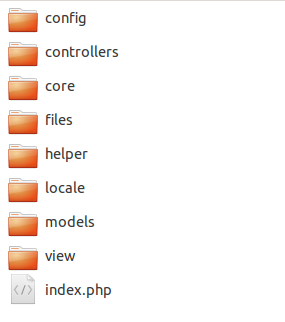
\includegraphics[width=4cm]{immagini/f12doc/a.png}
        \caption{Esempio di \textit{filesystem}}
    \end{figure}
    I Componenti principali del \textit{framework} saranno i seguenti:
        \begin{itemize}
            \item \textbf{Router:} il \textit{router} si trova all'interno della cartella core ed è una classe che si occupa di rimappare le richieste HTTP a chiamate alle azioni dei \textit{controller}. Inizialmente implementeremo un \textit{router} nel quale andranno registrate esplicitamente le mappature tra URL e azioni; successivamente estenderemo il concetto ed implementeremo un \textit{router} che analizzerà determinate directory del \textit{filesystem} per recuperare, in base all'URL richiesto, il \textit{controller} corretto;
            
            \item \textbf{Controller:} si trovano all'interno della cartella \textit{controllers} e rappresentano un insieme di azioni che potrebbero essere intraprese dall'utente. Ogni azione verrà rappresentata da un metodo definito nelle classi che estenderanno \textit{controller}; i metodi verranno richiamati in base a determinate condizioni e dovranno restituire una stringa che verrà inviata in output all'utente (solitamente una View renderizzata);
            
            \item \textbf{Models:} si trovano dentro la cartella models e si occupano dell'interfacciamo con il database. All'interno di models vengono fatte le query ed estratti i dati che poi verranno passati ai \textit{controller} e di conseguenza alle view. Solo dai \textit{controller} è possibile richiamare i metodi implementati all'interno dei models;
            
            \item \textbf{View:} si trovano nella cartella view e sono responsabili di visualizzare i dati dei modelli direttamente all'utente aggiungendo della grafica e del testo che rendano comprensibili i dati visualizzati;
            
            \item \textbf{Template:} rappresenta un template che verrà utilizzato come contenitore per renderizzare i dati assegnati in fase di costruzione;
            
            \item \textbf{Helper:} sono delle \textit{utility} utilizzate dalle view per poter formattare i dati presentati all'utente finale.
        \end{itemize}
    Esempio di richiesta http del \textit{framework}:
    \begin{figure}[!h] 
        \centering 
        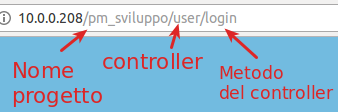
\includegraphics[width=8cm]{immagini/f12doc/b.png}
        \caption{Esempio di richiesta http}
    \end{figure}
    Ogni richiesta http che arriva al \textit{framework} contiene tutte le informazioni necessarie a renderizzare la pagina richiesta. Il \textit{router} si occupa di interpretare la richiesta php e scomporla per poter inizializzare l'opportuno \textit{controller} (nell'esempio stiamo invocando il \textit{controller} user) e invocare il metodo richiesto.
    \\
    L'esempio sopra riportato mostrerà la pagina di login del \textit{framework}.

\subsubsection{Bootstrap}
Bootstrap è una raccolta di strumenti liberi per la creazione di siti e applicazioni per il Web.
\begin{figure}[!h] 
    \centering 
    
\includegraphics[width=4cm]{immagini/loghi/bootstrap.png}
    \caption{Logo Bootstrap}
\end{figure}
\\
Contiene modelli di progettazione basati su HTML e CSS, sia per la tipografia,
che per le varie componenti dell'interfaccia, come moduli, pulsanti e navigazione,
così come alcune estensioni opzionali di JavaScript. Inizialmente si presentava come un progetto interno a Twitter, ma successivamente è diventato indipendente ed è perciò utilizzabile liberamente dagli sviluppatori come base per la realizzazione di interfacce web. Al momento è considerato il più efficiente ed il più utilizzato framework per rendere i siti web responsive. La versione usata nel progetto è Bootstrap 3.

\subsubsection{JQuery}
jQuery è una libreria JavaScript per applicazioni web. Nasce con l'obiettivo di semplificare la selezione, la manipolazione, la gestione degli eventi e l'animazione di elementi DOM in pagine HTML, nonché implementare funzionalità AJAX.
\\
Le sue caratteristiche permettono agli sviluppatori JavaScript di astrarre le interazioni a basso livello tra interazione e animazione dei contenuti delle pagine. L'approccio di tipo modulare di jQuery consente la creazione semplificata di applicazioni web e versatili contenuti dinamici.
\begin{figure}[!h] 
    \centering 
    
\includegraphics[width=4cm]{immagini/loghi/jquery.png}
    \caption{Logo JQuery}
\end{figure}
\\
È un software libero, distribuito sotto i termini della Licenza MIT e nel 2018, jQuery risulta la libreria JavaScript più utilizzata su Internet.

\subsubsection{DataTables}
Realizzato come plugin di jQuery, DataTables trasforma una comune tabella HTML aggiungendo tutte le caratteristiche richieste. DataTables utilizza il principio detto del \textit{progressive enhancement}, ossia se per qualche ragione il javascript non viene caricato, la tabella viene comunque resa in HTML standard ed è quindi pienamente fruibile.
\\
L'utilizzo delle DataTables è dovuto alla necessità di dover creare, all'interno pagine web, delle tabelle di dati interattive: filtrabili, ordinabili e paginate.

\subsubsection{EasyAutocomplete}
Una delle caratteristiche più utili e apprezzate per un motore di ricerca è sicuramente la sua capacità di offrire dei suggerimenti a chi effettua una ricerca.
\\
Una libreria molto completa e semplice da usare è EasyAutocomplete. Supporta suggerimenti da locale o remoto in \emph{JSON}\glsfirstoccur, \emph{XML}\glsfirstoccur e \textit{plain text}. 
Si fa apprezzare anche per la chiarezza della documentazione oltre alla semplicità di utilizzo essendo un \emph{plugin}\glsfirstoccur di jQuery.
\\
Di seguito viene riportato un esempio di \textit{script} realizzato da me per offrire all'utente tutte le possibilità di proprietario di protocollo in base alla tipologia selezionata.
\label{EasyAutocomplete}
\begin{lstlisting}[language=HTML, caption=HTML per \textit{EasyAutocomplete}]
    <div class="row">
        <div class="col-md-6">
            <div class="form-group form-reg">
                <label for="tipologia-intestatario">Tipologia proprietario</label>
                    <select class="form-control tipo-prop required" id="tipo-prop" name="tipo_proprietario">
                        <option></option>
                        <option value="C">Cliente</option>
                        <option value="F">Fornitore</option>
                        <option value="K">Contatto</option>
                        <option value="N">Nuovo Contatto</option>
                    </select>
                </div>
            </div>
            <div class="col-md-6">
                <div class="form-group form-reg">
                    <label for="nome-intestatario">Nome proprietario</label>
                    <input class="form-control general-autocomplete nome-proprietario" id="upper" extra-params="tipo-prop" data-url="<?php echo SITE_ROOT?>/protocolli/getSco"  name="nome_proprietario" disabled>
                </div>
            </div>
        </div>
    </div>
\end{lstlisting}
\begin{lstlisting}[language=Java, caption=JavaScript per EasyAutocomplete]
$('.general-autocomplete').each(function (){
    var dataType = 'json';
    var minLength = 2;
    var appendTo = '#container';
    var extraParams = '';

    if($( this ).attr('data-type'))
        dataType = $( this ).attr('data-type');

    if($( this ).attr('min-length'))
        minLength = $( this ).attr('min-length');

    if($( this ).attr('append-to'))
        appendTo = $( this ).attr('append-to');

    var url = $( this ).attr('data-url');

    var existextraparam = false;
    if($( this ).attr('extra-params'))
        existextraparam = true;

    var input = $(this);


    $( this ).autocomplete({
        source: function(request, response) {
            $.ajax({
                url: url+ (existextraparam ? componiurl(input.attr('extra-params')) : ''),
                dataType: "json",
                data: {
                    term : request.term
                },
                success: function(data) {
                    response(data);
                }
            });
        },
        type: "POST",
        minChars: minLength,
        dataType: dataType,
        data: {'tipo':$('#tipo-prop').val()},
        onSearchStart: function (query) {
            showOverlay();
        },
        onSearchComplete: function (query, suggestions) {
            hideOverlay();
        }
    });
});

function componiurl(idparam) {
    return '?' + $('#'+idparam).attr('name') + '=' + $('#'+idparam).val();
}
\end{lstlisting}
\newpage

%**************************************************************
\subsection{Formato per l'interscambio di dati}
\subsubsection{Array}
Un array può essere considerato come una collezione di elementi ognuno identificato da un indice; gli indici di un array possono essere numerici o stringhe. Gli elementi dell'array possono contenere al proprio interno qualsiasi tipo di dato, compresi oggetti o altri array.
\\
Grazie a quanto detto un metodo valido ed intuitivo per l'interscambio di dati è quello mediante array.
\subsubsection{JSON}
JSON ("JavaScript Object Notation") è un formato di scambio dati leggero e facile da leggere e scrivere per le macchine e di non difficile interpretazione per gli umani.
\begin{figure}[!h] 
    \centering 
    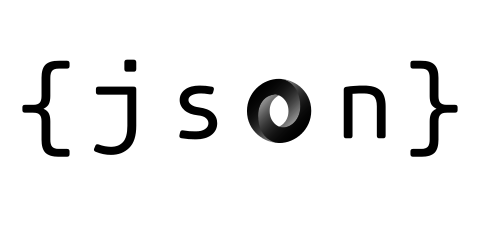
\includegraphics[width=6cm]{immagini/loghi/json.png}
    \caption{Logo JSON}
\end{figure}
\\
Si basa su un sottoinsieme del linguaggio di programmazione JavaScript, anche se ne è indipendente, ed inoltre è un formato di testo completamente indipendente da qualsiasi linguaggio. Per queste caratteristiche è un linguaggio di scambio dati ideale. 
\\
JSON è costruito su due strutture:
\begin{itemize}
    \item una collezione di coppie nome/valore, spesso realizzato come un array associativo;
    
    \item un elenco ordinato di valori, spesso realizzato come una lista.
\end{itemize}
Nel progetto esso è stato usato per poter scambiare i dati tra il lato front-end e il lato back-end, scambio che avviene con il passaggio di oggetti JSON.

%**************************************************************
\section{Strumenti utilizzati}
\label{sec:ciclo-vita-software}

\subsection{Ambiente di lavoro}
\subsubsection{macOS High Sierra - Versione 10.13.6}
Durante lo sviluppo del progetto, lo stagista ha utilizzato la versione di macOS High Sierra Versione 10.13.6.

Questa è la quattordicesima versione del sistema operativo macOS sviluppato da Apple Inc., la seconda a chiamarsi "macOS" invece che "OS X". È stato presentato ufficialmente al pubblico il 5 giugno 2017 a San Francisco. Lo stesso giorno della presentazione è uscita la prima beta per sviluppatori.

\subsubsection{PHPStorm}
PhpStorm è un \emph{IDE}\glsfirstoccur multipiattaforma commerciale per PHP basato sulla piattaforma IntelliJ IDEA di JetBrains.
\\
PhpStorm fornisce un editor per PHP, HTML e JavaScript con analisi del codice in tempo reale, prevenzione degli errori e \emph{refactoring}\glsfirstoccur automatizzati per codice PHP e JavaScript. Include un editor SQL che fornisce query modificabili.
\\
PhpStorm è costruito su IntelliJ IDEA, che è scritto in Java. Gli utenti possono estendere l'IDE installando plugin creati per la piattaforma IntelliJ o scrivendo i propri plugin.
\\
Tutte le funzionalità disponibili in WebStorm sono incluse in PhpStorm, che aggiunge il supporto per PHP e database.

\subsubsection{SQuirreLSQL}
SQuirreL SQL è uno strumento di amministrazione di database, gratuito e \textit{open source}, distribuito tramite licenza GNU.
\\
E' un \textit{client} che usa \textit{driver} JDBC per permettere all'utente di esplorare e interagire con un DBMS di diverso tipo. È provvisto di un editor SQL che offre il completamento automatico del codice.
\\
Può essere usato per:
\begin{itemize}
    \item aprire, creare, salvare ed eseguire script SQL;
    
    \item confrontare dati e condividere SQL statements tra i database.
\end{itemize}

\subsection{Ticketing}
Trello (vedi logo in Figura 3.16) è lo strumento di \textit{project management} utilizzato dall'azienda per gestire ed assegnare le attività da svolgere.
\begin{figure}[!h] 
    \centering 
    
\includegraphics[width=6cm]{immagini/loghi/trello.png}
    \caption{Logo Trello}
\end{figure}
Questo strumento permette di avere sempre traccia delle attività svolte e da svolgere, oltre che ad un coordinamento costante e non invasivo tra i vari membri del team. In questa piattaforma è infatti possibile costruire il proprio flusso di gestione degli sprint e tutte le attività correlate, così come pianificare il lavoro per la settimana successiva e sapere dove è collocato ogni componente del team. Trello, oltre che alla versione web, offre anche un'applicazione mobile.

\subsection{Documentazione}
L'azienda non stabilisce vincoli per quanto riguarda gli strumenti da usare per la produzione di documenti. La mia scelta è ricaduta su \LaTeX, un linguaggio di markup usato per la preparazione di testi, basato sul programma di composizione tipograca TEX.
\begin{figure}[!h] 
    \centering 
    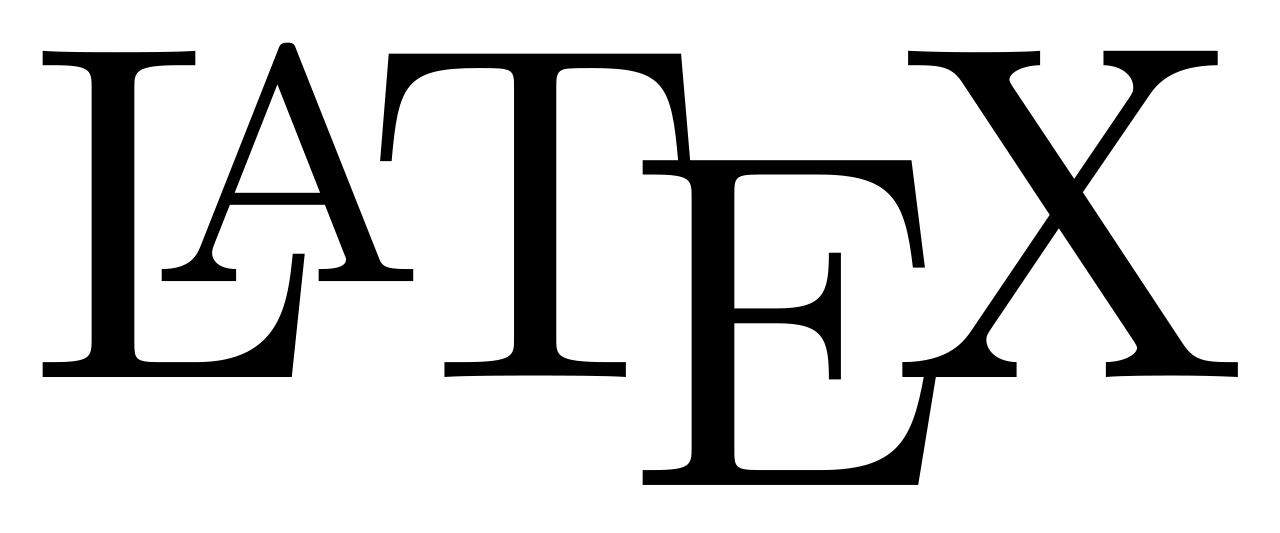
\includegraphics[width=6cm]{immagini/loghi/latex.png}
    \caption{Logo \LaTeX}
\end{figure}
\LaTeX presenta caratteristiche di stabilità e qualità al di sopra dei comuni \emph{wordprocessor}\glsfirstoccur in commercio, soprattutto per quanto riguarda la realizzazione di complesse tabelle o formule matematiche. 
\\
Inoltre, può essere esteso ed ampliato mediante diversi pacchetti. È distribuito con una licenza di software libero e questo lo ha reso disponibile per praticamente qualsiasi architettura: ne esistono pertanto versioni funzionanti per tutti i sistemi operativi, tra cui anche Microsoft Windows, macOS e le varie distribuzioni Linux.

\subsection{Strumenti di analisi statica e dinamica del codice}
\subsubsection{Psalm}
Psalm è uno strumento di analisi statica dedicato all'ambiente di sviluppo PHP che permette di \textit{debuggare} il codice scritto nel linguaggio \textit{serverside} più utilizzato al Mondo. Psalm permette di mantenere alto il livello di qualità del codice, specialmente se condiviso da un gruppo di persone, monitorando e prevenendo gli errori di \textit{runtime}.
\\
Psalm cerca, nella migliore maniera possibile data dal suo algoritmo interno, di interpretare ogni singola riga di codice per scovare svariate tipologie di errore. Oltre a questa caratteristica, tipica degli strumenti di analisi statica e di debugging di codice, Psalm offre funzionalità personalizzate come:
\begin{itemize}
    \item tenere traccia delle operazioni logiche del codice, producendo notifiche nei casi in cui si incontrano determinate asserzioni;
    
    \item controllare che tutte le proprietà di un dato oggetto abbiano un valore assegnato dopo la chiamata alla funzione costruttore
    
    \item supportare une formato che comprende gli array “object like”, permettendo di specificare il tipo delle chiavi degli stessi array.
\end{itemize}

\subsubsection{PHPUnit}
PHPUnit è un framework che oltre a fornire delle interfacce di base per scrivere \textit{Unit Test}, implementa anche una serie di funzionalità aggiuntive estremamente utili che aiutano a scrivere test ben ordinati ed assolutamente efficienti.
\\
PHPUnit si basa sull'idea che gli sviluppatori dovrebbero essere in grado di trovare rapidamente errori nel loro codice appena eseguito e affermare che nessuna regressione del codice si è verificata in altre parti del codice di base. Proprio come gli altri framework di \textit{Unit Test}, PHPUnit utilizza asserzioni per verificare che il comportamento del componente specifico in fase di test si comporti come previsto.
%**************************************************************
\section{Ciclo di vita del software}
\label{sec:ciclo-vita-software}
Il modello adottato per la realizzazione del progetto è quello a spirale in quanto permette di scomporre il processo di sviluppo in quattro fasi multiple, ciascuna ripetuta più volte.
\\
Queste fasi sono:
\begin{itemize}
    \item \textbf{Pianificazione:} nella pianificazione si determinano degli obiettivi, delle alternative e i vincoli associati al progetto. Il committente e il fornitore del sistema interagiscono allo scopo di definire in maniera sufficientemente univoca cosa deve essere realizzato e come. In questa fase è buona norma redigere dei documenti, in principio non eccessivamente dettagliati, che fissino i punti fondamentali della pianificazione del lavoro futuro;
    
    \item \textbf{Analisi dei rischi:} Nell'analisi dei rischi si identificano e si analizzano i problemi e i rischi associati al progetto, al fine di determinare delle strategie per controllarli;
    
    \item \textbf{Sviluppo:} Nella fase di sviluppo si procede alla vera e propria realizzazione: i tempi di realizzazione di questa attività, che comprende sia la codifica sia la verifica, sono tra i più lunghi tra tutti quelli previsti all'interno del ciclo di vita del prodotto software;
    
    \item \textbf{Valutazione:} Nella fase di valutazione il committente valuta se il sistema realizzato risponde alle sue esigenze. Attraverso questa fase il committente verifica che il prodotto soddisfi effettivamente i requisiti richiesti. Una logica conseguenza del fatto che un prodotto software non superi la fase di validazione dei requisiti è la necessità di impostare un nuovo ciclo di attività.
\end{itemize}

%**************************************************************
\section{Progettazione}
\label{sec:progettazione}
    L’architettura generale del software è costituita da un \emph{\textit{frontend}\glsfirstoccur}, da un \emph{\textit{backend}\glsfirstoccur} e da un database che si occupa di mantenere la persistenza dei dati.
    \\
    \\
    Il \emph{\textit{Design pattern}\glsfirstoccur} adottato per la realizzazione dell'applicativo è l'\emph{\textit{MVC}\glsfirstoccur} che è un pattern architetturale molto diffuso nello sviluppo di sistemi software, in particolare nell'ambito della programmazione orientata agli oggetti, in grado di separare la logica di presentazione dei dati dalla logica di business.
    \begin{figure}[!h] 
        \centering 
        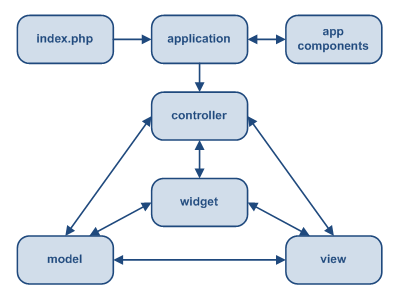
\includegraphics[width=10cm]{immagini/structure.png}
        \caption{Struttura architettura}
    \end{figure}
    \newpage
    Le funzioni del \textit{controller} che hanno lo stesso nome della \textit{view} si occupano della renderizzazione di quest'ultima grazie alla chiamata della funzione \texttt{render(\$view, \$template)} che richiede come parametri il nome della view e il \textit{template} di \textit{view} che si vuole renderizzare. Queste funzioni si occupano anche di restituire alla \textit{view} i dati prelevati mediante apposite \textit{query} contenute nella classe \textit{protocollimodel} nel model.
    
    \subsection{Dashboard}
    Per ottenere la pagina di visualizzazione della lista di protocolli, il più fedele possibile a quanto richiesto, le funzioni da realizzare saranno:
    
    \subsubsection{\texttt{daschboard()}}
    Questa funzione si occupa della renderizzazione della pagina "Dashboard" e si interfaccia con il database mediante la query contenuta in \texttt{getProtocolsToSeeForUser(\$user)} per ricordare all'utente quanti protocolli deve ancora visionare.
    
    \subsubsection{\texttt{getProtocolsForAdmin()}}
    Questa funzione popola la \textit{datatable} nella dashboard di un amministratore che può vedere ed elaborare tutti i protocolli inseriti nel sistema. La stessa si interfaccia con il database mediante la query contenuta nella funzione \texttt{getProtocolsForAdmin()} in \textit{protocollimodel}.
    
    \subsubsection{\texttt{getProtocols()}}
    Questa funzione popola la \textit{datatable} della dashboard di un utente normale che può visionare ed elaborare solo i protocolli a lui attribuiti o da lui inseriti. La stessa si interfaccia con il database mediante la query contenuta nella funzione \texttt{getProtocolliForUsers()} in \textit{protocollimodel}.
    
    %registrazioneprotocollo
    \subsection{Registrazione protocollo}
    Per permettere ad utente di registrare un protocollo le funzioni da realizzare saranno:
    
    \subsubsection{\texttt{protocolRegistration()}}
    Questa funzione si occupa della renderizzazione della pagina "Registrazione Protocollo" e si interfaccia con il database per la generazione automatica di codici progressivi ed univoci quali codice seriale e codice a barre. 
    Le due \textit{query} sono rispettivamente contenute nelle funzioni \texttt{codeGenerator(\$register)} e \texttt{barcodeGenerator()} situate all'interno di \textit{protocollimodel}.
    \\
    La funzione si occupa inoltre di creare un array associativo dei risultati ottenuti dalle \textit{query} contenute nelle funzioni \texttt{getFromDomd()} e \texttt{getFromDprt()}.
    Questo array permette di attribuire ad ogni tipologia di protocollo esistente i suoi corrispettivi metadati.
    
    \subsubsection{\texttt{getSco()}}
    Questa funzione si interfaccia con il database mediante la funzione \texttt{searchSco(\$type, \$search)} che prende come parametri la tipologia di proprietario a cui si vuole intestare il protocollo e la iniziali del nome dell'intestatario del medesimo protocollo. 
    \\
    La stessa è utilizzata per restituire i suggerimenti mediante la funzione che utilizza \textit{EasyAutocomplete} riportata nel paragrafo \hyperref[EasyAutocomplete]{EasyAutocomplete}
    
    \subsubsection{\texttt{nextProtocol(\$register)}}
    Questa funzione viene chiamata al variare della selezione del registro di appartenenza e si occupa di creare un JSON contenente il codice seriale corrispondente al nuovo registro selezionato.
    
    \subsubsection{\texttt{addProtocol()}}
    Questa funzione viene chiamata alla selezione del tasto \textit{submit} e si occupa di salvare nelle rispettive tabelle del database i dati inseriti nel form di registrazione di un nuovo protocollo.
    
    %detailPage
    \subsection{Visualizzazione protocollo}
    Per permettere ad un utente di consultare le informazioni riguardanti un protocollo le funzioni da realizzare saranno:
    
    \subsubsection{\texttt{detailPage(\$serial\_code)}}
    Questa funzione si occupa della renderizzazione della pagina "Dettaglio protocollo" e si interfaccia con il database mediante le seguenti funzioni:
    \begin{itemize}
        \item \texttt{getProtocol(\$protocolcod)} per restituire tutte le informazioni riguardanti il protocollo passato come parametro della funzione;
        
        \item \texttt{getMetadatiPerProtocollo(\$protocolcod)} per restituire tutti i metadati assegnati al protocollo passato come parametro della funzione;
        
        \item \texttt{getAddettiConDataChiusuraAtut(\$typecod, \$serialcode)} per restituire tutti gli operatori assegnati all'elaborazione del protocollo.
    \end{itemize}
    Questa funzione si occupa inoltre di prelevare dall'archivio "F12 Documentale" il documento allegato al protocollo in fase di registrazione del medesimo.
    
    \subsubsection{\texttt{findMatch()}}
    Questa funzione permette di accedere alla pagina di dettaglio di un protocollo mediante lo \textit{scan} di codice a barre. Per fare in modo che ciò avvenga viene chiamata la funzione \texttt{getProtocolFromBarcode(\$barcode)} che mediante \textit{query} preleva dal database il protocollo avente come barcode il codice scansionato.
    
    \subsubsection{\texttt{updateClosingAtut()}}
    Questa funzione permette di aggiornare lo stato di un protocollo quando l'utente dichiara di averlo visionato. Verrà fatto un update del campo dedicato impostando come valore la data e l'ora in cui l'utente ha marcato come visionato tale protocollo.
    
    \subsubsection{\texttt{saveChat()}}
    Questa funzione permette di salvare e visualizzare istantaneamente un messaggio inserito nella sezione "Timeline e Commenti".
    
    %sendMail
    \subsection{Invia e-mail}
    Per consentire l'invio di un protocollo tramite posta elettronica le funzioni da realizzare saranno:
    
    \subsubsection{\texttt{sendMail(\$serial\_code)}}
     Questa funzione si occupa della renderizzazione della pagina "Invia mail" e si interfaccia con il database mediante la funzione \texttt{getIndirizzi(\$codice)} per proporre all'utente gli indirizzi del personale interno o dell'intestatario del protocollo.
    
    \subsubsection{\texttt{send()}}
    Questa funzione viene chiamata alla selezione del tasto "Invia" e si occupa di inviare la mail al destinatario selezionato usando la funzione \texttt{sendMail(\$to, \$from, \$object, \$msg, \$file)}
    
    %typeConfiguration
    \subsection{Registrazione protocollo}
    Per permettere ad un utente la facile consultazione di tipologie esistenti o per crearne di nuove le funzioni da realizzare saranno:
    
    \subsubsection{\texttt{typeConfiguration()}}
    Questa funzione si occupa della renderizzazione della pagina "Configurazione tipologia protocollo" e si interfaccia con il database mediante le seguenti funzioni:
    \begin{itemize}
        \item \texttt{codDotiGenerator()} per la generazione del codice univoco della nuova configurazione;
        \item \texttt{getGruppi()} per restituire come \textit{option} tutti gli uffici esistenti;
        \item \texttt{getUtentiFromGruppo(\$office)} per restituire tutti gli operatori facenti parte dell'ufficio selezionato.
    \end{itemize}
    
    \subsubsection{\texttt{nextGroup()}}
    Questa funzione viene chiamata quando un'utente dichiara di voler aggiungere un nuovo ufficio, con rispettivo personale, addetto all'elaborazione del documento. 
    \\
    Questa si occupa di creare un JSON contenente tutti gli uffici registrati nel database tranne quelli già selezionati.
    
    \subsubsection{\texttt{nextUsers(\$group)}}
    Questa funzione si occupa di creare un JSON contenente tutti gli operatori facenti parte dell'ufficio selezionato.
    
    \subsubsection{\texttt{getConfig()}}
    Questa funzione popola la \textit{datatable} che mostra all'utente tutte le tipologie esistenti. La stessa si interfaccia con il database mediante la query contenuta nella funzione \texttt{getConfiguration()} in \textit{protocollimodel}.
    
    \subsubsection{\texttt{addConfig()}}
    Questa funzione viene chiamata alla selezione del tasto \textit{submit} e si occupa di salvare nelle rispettive tabelle del database i dati inseriti nel form per la creazione di una nuova tipologia di protocollo.
    
    %typeConfigurationDetail
    \subsection{Visualizzazione tipologia}
    Per permettere ad un utente di consultare le informazioni riguardanti una tipologia di protocollo le funzioni da realizzare saranno:
    
    \subsubsection{\texttt{typeConfigurationDetail(\$type\_code)}}
    Questa funzione si occupa della renderizzazione della pagina "Dettaglio configurazione" e si interfaccia con il database mediante le seguenti funzioni:
    \begin{itemize}
        \item \texttt{getMetadati(\$protocolscod)} per restituire tutti i metadati assegnati alla tipologia di cui si sta visionando i dettagli;
        
        \item \texttt{getNumDocumentByTipol(\$protocolscod)} per controllare se nel database ci sono protocolli con la tipologia corrispondente a quella in esame. Questo controllo viene fatto per permettere o meno all'utente di eliminare una tipologia;
        
        \item \texttt{getAddetti(\$protocolscod)} per restituire tutti gli operatori addetti all'elaborazione della tipologia in esame;
        
        \item \texttt{getGroup()} per restituire tutti gli uffici di cui gli operatori addetti fanno parte. 
    \end{itemize}
    
    \subsubsection{\texttt{reset()}}
    Questa funzione viene chiamata alla selezione del tasto "Reset" nella pagina di dettaglio della tipologia e fa la \textit{delete} nel \textit{database} di tutti gli operatori assegnati a quella tipologia.
    
    \subsubsection{\texttt{addNewOperators()}}
    Questa funzione viene chiamata alla selezione del tasto "submit" nella pagina di dettaglio della tipologia e permette di inserire nuovi operatori addetti all'elaborazione della tipologia in esame.
    
    \subsubsection{\texttt{addNewMeta()}}
    Questa funzione viene chiamata alla selezione del tasto "submit" nella pagina di dettaglio della tipologia e permette di inserire nuovi metadati alla tipologia in esame.
    
    \subsubsection{\texttt{deleteConfig()}}
    Questa funzione viene chiamata alla selezione del tasto "Elimina" nella pagina di dettaglio della tipologia e permette di eliminarela configurazione in esame.

%**************************************************************
\section{Codifica}
%**************************************************************
\subsection{Dashboard}

    \subsubsection{Codice}
        Nella pagina denominata \textit{Dashboard} si può visualizzare l'elenco di tutti i protocolli assegnati ad un operatore o registrati dal medesimo operatore.
        \\ 
        L'elenco è stato realizzato utilizzando una \textit{DataTable} ed è popolato mediante \textit{query} che oltre alla \textit{select} dei protocolli si occupa anche dei filtri mediante i quali si può ricercare un protocollo o un gruppo di di protocolli.
        \\
        I filtri sono stati realizzati mediante la concatenazione di condizioni derivanti dall'input dell'utente.
        
        \begin{lstlisting}[language=SQL, caption=Query per Dashboard]
public function getProtocolliForUsers($Dadate, $Adate, $reg, $tipol, $prop, $ope, $fname, $loggedope) {
    $condizione = "";
    if ($Dadate != "")
        $condizione .= " AND dpro_data >= '$Dadate'";
    if ($Adate != "")
        $condizione .= " AND dpro_data <= '$Adate'";
    if ($reg != "")
        $condizione .= " AND dpro_registro = '$reg'";
    if ($tipol != "")
        $condizione .= " AND dpro_tipo = '$tipol'";
    if ($prop != "")
        $condizione .= " AND dpro_nome_prop LIKE '%".strtoupper($prop)."%'";
    if ($ope != "")
        $condizione .= " AND dpro_operatore = '$ope'";
    if ($fname != "")
        $condizione .= " AND dpro_filename_scan LIKE '%$fname%'";

    $sql = "SELECT dpro.*, dprt_descri, dprt_cod_doti  
            FROM dpro, dprt
            WHERE dpro_tipo = dprt_codice
            AND dpro_operatore = '$loggedope' $condizione
            UNION
            SELECT dpro.*, dprt_descri, dprt_cod_doti  
            FROM dpro, dprt, dpru
            WHERE dpro_tipo = dprt_codice
            AND dprt_cod_doti = dpru_codice
            AND dpru_cod_utente = '$loggedope' $condizione
            UNION
            SELECT dpro.*, dprt_descri, dprt_cod_doti  
            FROM dpro, dprt, dpru, usbg
            WHERE dpro_tipo = dprt_codice
            AND dprt_cod_doti = dpru_codice
            AND dpru_cod_gruppo = usbg_group
            AND usbg_operatore = '$loggedope' 
            AND dpru_cod_utente = '' $condizione";
    $res = $this->query($sql);
    return $res;
}
        \end{lstlisting}
        
        
        Il risultato della \textit{query} viene poi elaborato dalla funzione \textit{getProtocols()} che mediante \textit{array} attribuisce ad ogni colonna della \textit{DataTable} il corrispondete valore. 
        \\
        Infine l'\textit{array} viene convertito in formato JSON per essere elaborato dalla \textit{DataTable}.
        \begin{lstlisting}[language=PHP, caption=Funzione getProtocols()]
public function getProtocols(){
    $Dadate='';
    $Adate='';
    $reg='';
    $tipol='';
    $prop='';
    $ope='';
    $fname='';
    foreach ($_REQUEST['filters'] as $filter) {
        if($filter['name']=='Dadata'){
            $Dadate = $filter['value'];
        }
        if($filter['name']=='Adata'){
            $Adate = $filter['value'];
        }
        if($filter['name']=='registro'){
            $reg = $filter['value'];
        }
        if($filter['name']=='tipologia'){
            $tipol = $filter['value'];
        }
        if($filter['name']=='proprietario'){
            $prop = $filter['value'];
        }
        if($filter['name']=='operatore'){
            $ope = $filter['value'];
        }
        if($filter['name']=='filename'){
            $fname = $filter['value'];
        }
    }
    $protocolli = $this->model->getProtocolliForUsers($Dadate, $Adate, $reg, $tipol, $prop, $op$fname, $_SESSION[NOME_SESSIONE]['user']);
    $return['data'] = array();
    $i=0;
    foreach($protocolli as $p) {
        $return['data'][$i]['DT_RowId'] = $p->dpro_serial_doc;
        $return['data'][$i][0] = $p->dpro_serial_doc;
        $return['data'][$i][1] = $p->dpro_filename_scan;
        $return['data'][$i][2] = $p->dprt_descri." (".$p->dprt_codice.")";
        if ($p->dpro_registro == 'S'){
            $return['data'][$i][3] = "Spedito";
        } elseif ($p->dpro_registro == 'R'){
            $return['data'][$i][3] = "Ricevuto";
        } else {
            $return['data'][$i][3] = "Interno";
        }
        $return['data'][$i][4] = $p->dpro_operatore;
        $return['data'][$i][5] = $p->dpro_data;
        $return['data'][$i][6] = $p->dpro_barcode_tag;
        $return['data'][$i][7] = $p->dpro_nome_prop;
        $i++;
    }
    echo $this->mw_json_encode($return);
}
        \end{lstlisting}
        
    \subsubsection{Resa finale}
        È stata prestata molta attenzione alla presentazione grafica della pagina, cercando un'estetica semplice ma professionale.
        
        \begin{figure}[!h] 
            \centering 
            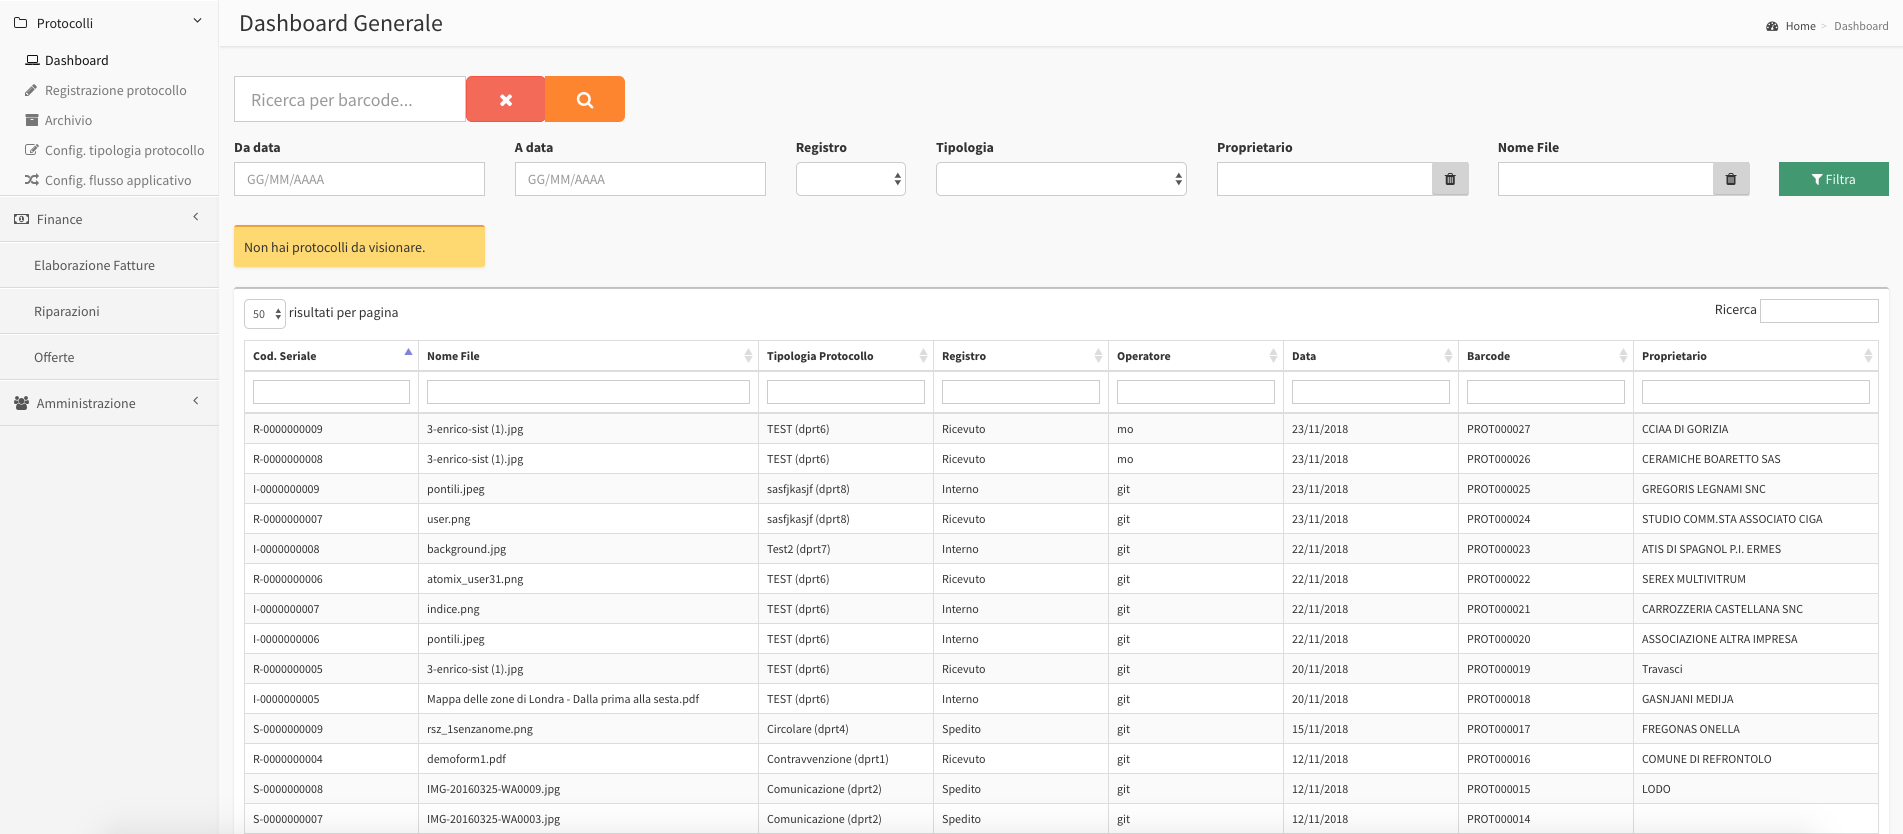
\includegraphics[width=\textwidth]{immagini/prodottofinito/dashboard.png}
            \caption{Dashboard view}
        \end{figure}
        \newpage
        L'\textit{header} della pagina è dedicata ai filtri. 
        \\
        Come richiesto dal requisito \hyperref[RFO6]{RFO6} sarà possibile, mettendo il \textit{focus} sul campo \textit{input} nominato "Ricerca per \textit{barcode}", accedere direttamente al dettaglio del protocollo di cui si è effettuato lo \textit{scan} del \textit{barcode}.
        \\
        Al di sotto di questo campo l'utente potrà filtrare i protocolli per tutti i campi visibili della \textit{DataTable}.

\subsection{Visualizzazione Protocollo}

    \subsubsection{Codice}
        Nella pagina di visualizzazione di un singolo protocollo oltre alle informazioni generali prelevate dal database mediante apposita \textit{query} viene inoltre presentata una preview del documento protocollato.
        \\
        Essendo il documento salvato nella piattaforma documentale "F12 Documentale", per essere stampato a video, bisogna seguire i seguenti \textit{step}:
        \begin{itemize}
            \item comporre il link dove il documento è contenuto;
            
            \item estrarre il contenuto del link appoggiandosi alla funzione \textit{file\_get\_contents()};
            
            \item decodificare il risultato JSON ottenuto;
        
            \item creare una cartella temporanea dove salvare temporaneamente il file d'interesse;
            
            \item creare la view per stampare il file in base alla tipologia dello stesso.
        \end{itemize}
        
        \begin{lstlisting}[language=PHP, caption=Pint della preview del documento]
//URL
$pathpreview = $this->model->getWSPathDocu('preview');
$wsdocupath = $pathpreview."/".$this->protocollo->dpro_docu_id."/";
    
//PERNDO IL CONTENUTO DELL'URL
$target = file_get_contents($wsdocupath);
    
//DECODE
$docs = json_decode($target);
$decoded = base64_decode($docs->doc);
    
    
//PRELEVO LE INFORMAZIONI DI INTERESSE
$mime = $docs->mime;
$name = $docs->name;
$this->desc = $docs->docd_descriz;
    
$this->pathdocumentotmp = SERVER_ROOT.'/files/tmp/'.$name;
    
if(!is_dir(SERVER_ROOT.'/files/tmp/')){
    $this->model->mw_mkdir(SERVER_ROOT.'/files/tmp/');
}
    
//IN BASE AL FILE DIVERSI TIPI DI VIEW
file_put_contents($this->pathdocumentotmp, $decoded);
$ppp = '';
if (exif_imagetype($this->pathdocumentotmp) != false) {
    $ppp.= '<div class="imagecontainer">';
    $ppp.= '<img style="width:100%;" src="' . SITE_ROOT.'/files/tmp/'.$name . '" >';
    $ppp.= '</div>';
} else if ($mime == 'application/pdf') {
    $ppp.= '<div class="imagecontainer">';
    $ppp.= '<iframe src="' . SITE_ROOT.'/files/tmp/'.$name . '" width="100%" height="600" ></iframe>';
    $ppp.= '</div>';
} else {
    $ppp.= '<div class="imagecontainer">';
    $ppp.= '<img id="myImg" style="width:100%;" src="' . SITE_ROOT . '/files/img/PNA.png" >';
    $ppp.= '</div>';
}
$this->prev = $ppp;
        \end{lstlisting}
    
    \subsubsection{Resa finale}
        \begin{figure}[!h] 
            \centering 
            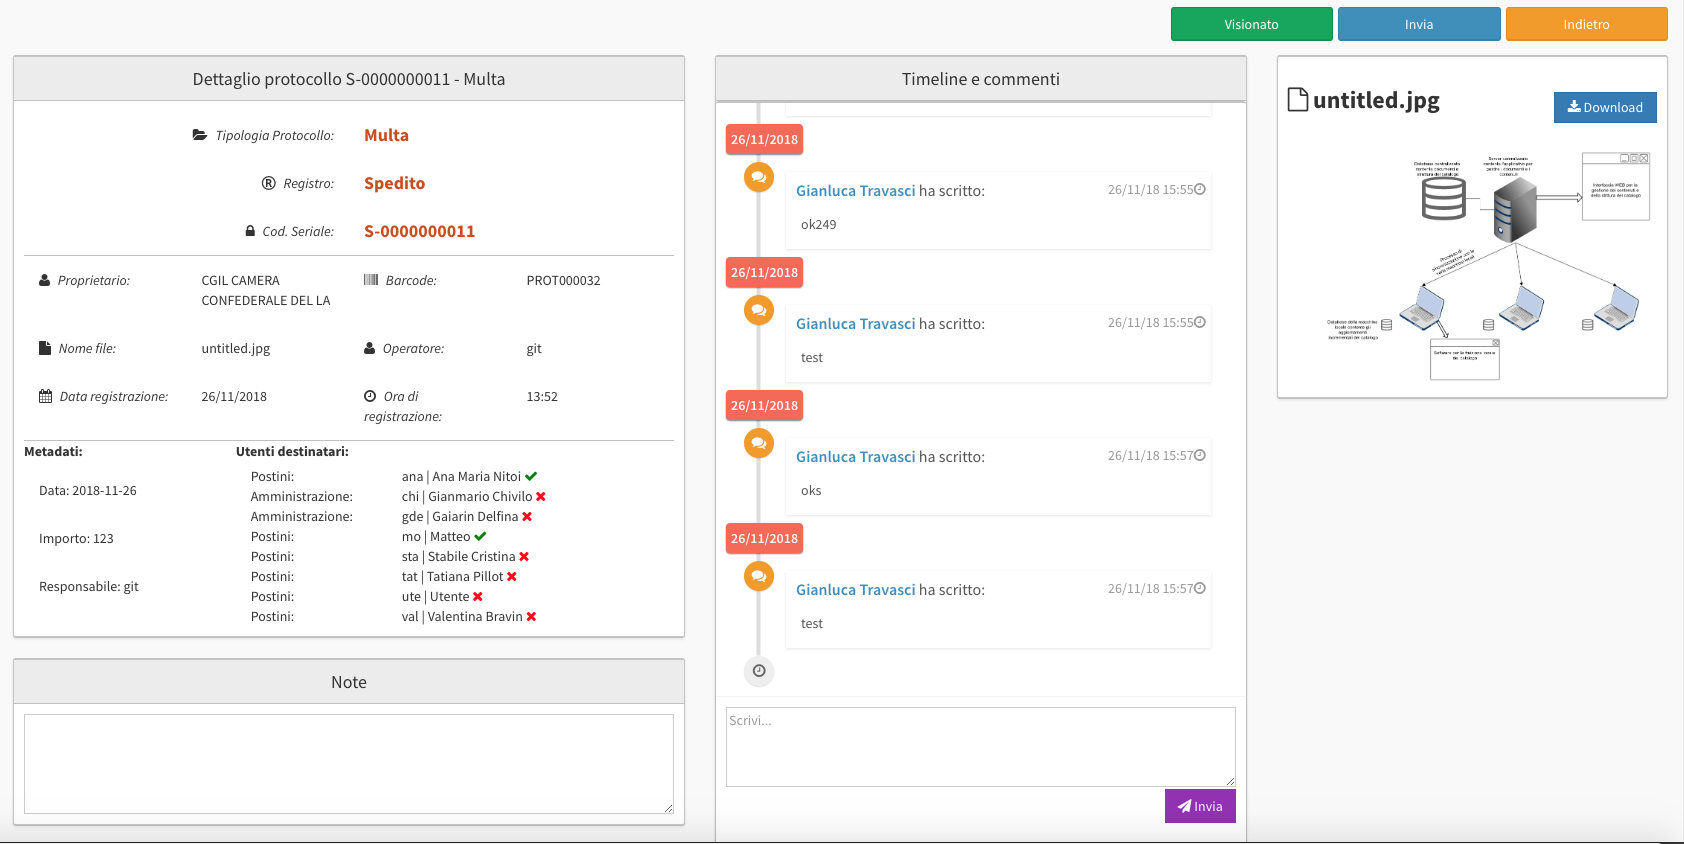
\includegraphics[width=\textwidth]{immagini/prodottofinito/dettproto.png}
            \caption{Dettaglio protocollo view}
        \end{figure}
       
        L'immagine in \textit{preview} è scaricabile mediante apposito bottone che si collega all'url per il download del documento sulla piattaforma "F12 Documentale".
        \\
        Ogni volta che viene registrato un protocollo viene creata una riga, per ogni utente coinvolto, nell'apposita tabella del \textit{database} con campo "chiusura \textit{task}" impostato di \textit{default} a null.
        \\
        Quando l'operatore asserisce di aver visionato il documento, premendo il bottone "Visionato", il campo "chiusura task" verrà aggiornato con la data e l'ora corrente e accanto al proprio nome comparirà una spunta verde.
        \\
        Questo salvataggio della data e dell'ora permette inoltre di tenere traccia dello storico del documento come richiesto dal requisito \hyperref[RFO3.1.11]{RFO3.1.11}.
        
\subsection{Registrazione Protocollo}
    \subsubsection{Codice}
        Al variare della tipologia di documento selezionata vengono stampati a video i campi metadato creati in fase di configurazione della tipologia. Per realizzare tale funzionalità è stata creata una \textit{query} che preleva dalla tabella dedicata ai metadati tutti quelli corrispondenti alla tipologia selezionata, quindi mediante script è stata eliminata la \textit{html class} che settava a \textit{"display: none"} e rendeva nascosti tali campi input.
        \\
        Lo stesso principio è stato adottato per la selezione della "Tipologia proprietario" e del "Nome Proprietario" nel caso in cui si selezioni "Nuovo Contatto".
        In questo caso, in fase di salvataggio, il valore del campo "Nome e Cognome (Azienda)" verrà salvato nella tabella delle informazioni sul protocollo sotto la voce "Nome Proprietario"
        \\
        Tutti i dati inseriti e visualizzati non modificabili, un volta premuto il bottone \textit{submit} della form di registrazione di un nuovo protocollo, vengono passati tramite una richiesta POST e sono disponibili lato server nella variabile \$\_POST. In seguito i dati vengono memorizzati nel database appoggiandosi alla funzione \textit{insert(\$dati, \$tabella)} presente nel \textit{framework} aziendale.
        \\
        Il documento caricato in fase di compilazione della form viene trasmesso mediante cURL al servizio "F12 Documentale" in cui verrà archiviato. 
       \newpage \begin{lstlisting}[language=PHP, caption=Upload su Documentale]
$pathdoc=$this->model->getPathDoc();
$urlpath = str_replace("/documentale/documentale/documentif12/","/documentale_coop/documentale/uploadfile", $pathdoc);
$url = $urlpath."?mask=".$funzione_accesso."&val=".$_POST['dpro_serial_doc']."&ope=".$_SESSION[NOME_SESSIONE]['user']['sigla']."&rowval=&db=dbf12&tipologia=".$_POST['dpro_tipo']."&external=1";

foreach($_FILES as $nome => $file) {

    if (trim($file['name']) != "") {
        $desc = isset($_REQUEST['desc']) ? $_REQUEST['desc'] : '';
        $curl = curl_init();

        $post_data = array('file' => '@' . $file['tmp_name'], 'name' => $file['name'], 'type' =$file['type'], 'dsc' => $desc);
        curl_setopt($curl, CURLOPT_POSTFIELDS, $post_data);

        // OPTIONS:
        curl_setopt($curl, CURLOPT_URL, $url);
        curl_setopt($curl, CURLOPT_RETURNTRANSFER, 1);
        curl_setopt($curl, CURLOPT_SSL_VERIFYPEER, false);

        // EXECUTE:
        $result = curl_exec($curl);
        curl_close($curl);
    }
}
        \end{lstlisting}
        Sulla variabile \textit{\$result} viene salvato il codice univoco della riga del database corrispondente al documento caricato. Il codice viene poi usato per fare l'\textit{update} del campo \textit{id\_documentale} nella riga della tabella dedicata alle informazioni del protocollo mettendo così le due tabelle in relazione "uno a uno".
    \subsubsection{Resa finale}
        \begin{figure}[!h] 
            \centering 
            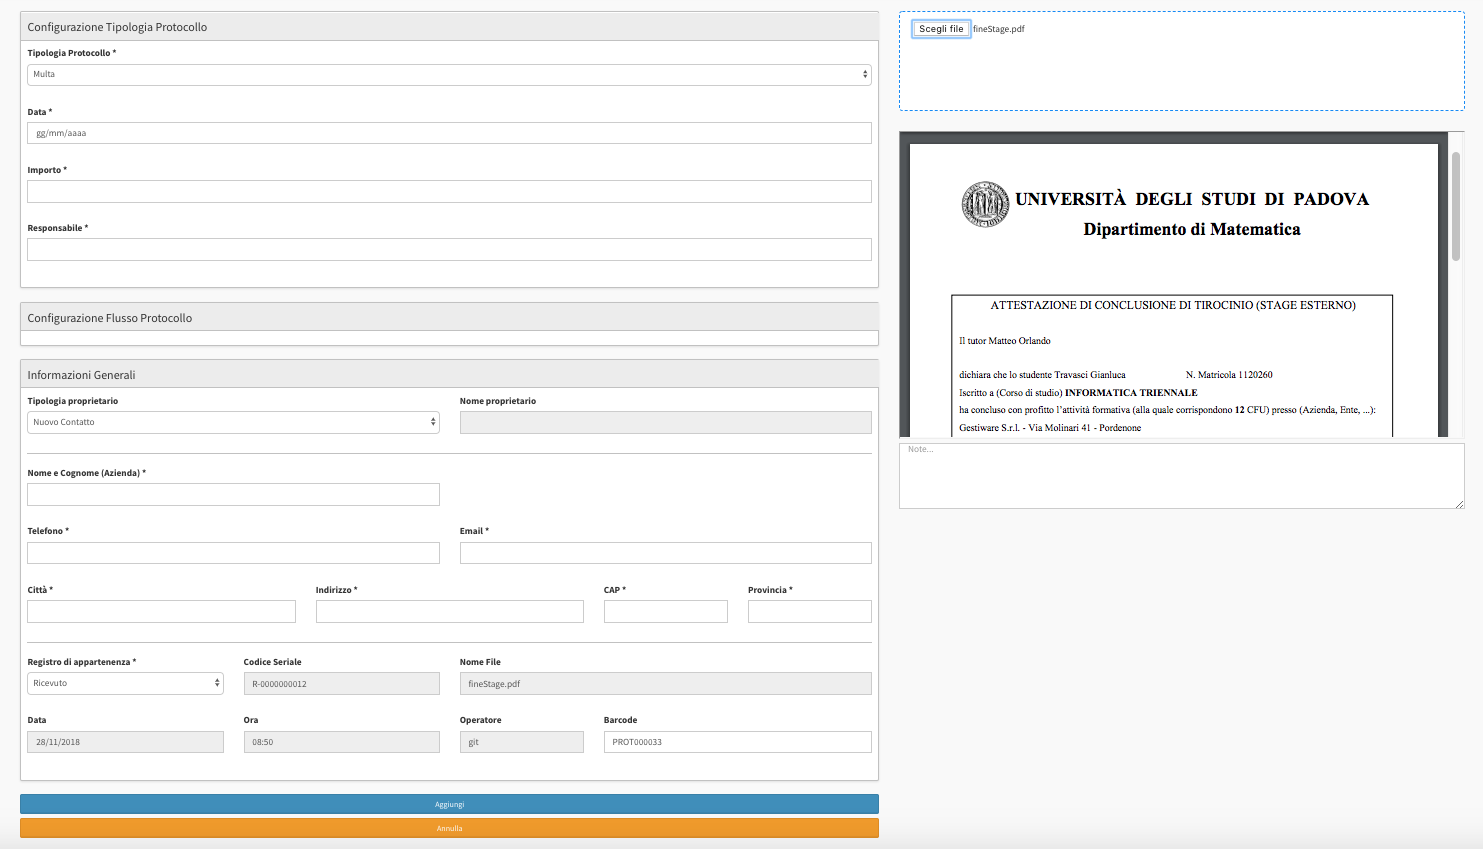
\includegraphics[width=\textwidth]{immagini/prodottofinito/regproto.png}
            \caption{Registrazione protocollo view}
        \end{figure}
        Come accennato precedentemente, selezionando "Nuovo Contatto" nella selezione della "Tipologia proprietario" il campo "Nome Proprietario" verrà disabilitato e comparirà la form di registrazione di un nuovo contatto.
        
\subsection{Configurazione della tipologia}
    \subsubsection{Codice}
        Come precedentemente descritto per la dashboard, per presentare tutte le tipologie esistenti è stata adottata una \textit{DataTable}.
        \\
        Per l'assegnazione degli operatori addetti all'elaborazione della tipologia di protocollo in fase di creazione sono state utilizzate due chiamate \textit{Ajax}.
        \\
        La prima è stata realizzata per far fronte all'esigenza di poter aggiungere utenti facenti parte di diversi uffici. Quando viene assegnato il primo ufficio con rispettivo personale e viene premuto il tasto "Aggiungi" viene effettuata la chiamata \textit{Ajax} e se essa ha successo viene fatto l'\textit{append} di una nuova riga di codice html.
        \\
        I dati da stampare nelle select vengo passati in formato JSON dalla funzione apposita nel \textit{controller} e vengono decodificati mediante funzione \textit{parseJSON(data)}.
        \\ 
        Premendo il tasto "Elimina" verrà eliminata la nuova riga aggiunta.
        \begin{lstlisting}[language=PHP, caption= JQuery per nuova riga]
var i=1;
$('#addgruppo').click(function(){
    i++;
    $.ajax({
        url: baseurl+'/protocolli/nextGruppi',
        success: function (data) {
            var parsed = $.parseJSON(data);
            console.log(parsed.gruppinext);
            var html='<div id="row'+i+'">' +
                    '<div class="col-md-5">'+
                        '<select class="form-control gruppi-esistenti required" id="'+i+'" name="gruppi[sezione][]">' +
                            '<option></option>';
                            $.each(parsed.gruppinext,function (i,v) {
                                    html+= '<option value="'+ v.uswg_codice +'">'+ v.uswg_descrizione +'</option>'
                            });
                        html += '</select>'+
                    '</div>' +
                    '<div class="col-md-5">'+
                        '<select class="form-control operatori-da-attribuire required" id="'+i+name="gruppi[contatti][]">' +
                            '<option></option>' +
                            '<option value="T">Tutti</option>' +
                            '<option value="S">Seleziona</option>' +
                        '</select>' +
                        '<div class="row hide" id="operatori-assegnabili-'+i+'">' +
                            '<div class="box box-nomi-'+ i +'" style="margin-top: 1em; padding-left: 5px;">' +
                            '</div>'+
                        '</div>'+
                    '</div>'+
                    '<div class="col-md-2">' +
                            '<button type="button" name="remove" id="'+i+'" class="btn btn-danger btn_remove_gruppo">Elimina</button>' +
                    '</div>' +
            '</div>';
            $('#aux').append( html );
        }
    });
});
$(document).on('click', '.btn_remove_gruppo', function(){
    var button_id = $(this).attr("id");
    $('#row'+button_id+'').remove();
});
        \end{lstlisting}
        
        La seconda chiamata \textit{Ajax} è stata realizzata per far fronte all'esigenza di poter selezionare solo alcuni utenti facenti parte di un ufficio. 
        \\ 
        Come nel caso della chiamata precedete i dati sono prelevati in formato JSON e sono decodificati con la funzione \textit{parseJSON(data)}.
        \\
        Se la chiamata \textit{Ajax} ha successo viene fatto l'\textit{append} di codice alla classe \textit{box-nomi} e il suddetto box viene visualizzato o meno in base all'opzione selezionata nella \textit{select} "Assegna Utenti".
        \begin{lstlisting}[language=PHP, caption= JQuery Nuovi utenti]
$(document).on('change','select.operatori-da-attribui',function() {
    var id = $(this).attr('id');
    if ($(this).val() == 'S') {
        $('#operatori-assegnabili-'+ i+'').removeClass('hide');
    } else {
        $('#operatori-assegnabili-'+ i+'').addClass('hide');
    }
});
            
$(document).on('change','select.gruppi-esistenti',function(){
    var select_id = $(this).attr("id");
    var get=$(this).val();
            
    $.ajax({
        url: baseurl+'/protocolli/nextUtenti/'+get,
        success: function (data) {
            var parsed = $.parseJSON(data);
            console.log(parsed.utentinext);
            var html='<div>';
            $.each(parsed.utentinext,function (i,v) {
                html+='<div class="row">' +
                    '<div class="col-md-1">' +
                     '<input type="checkboxclass="ablename="operatore-da-assegnare[]value=" '+ v.usbg_operatore +'">+
                    '</div>' +
                    '<div class="col-md-9">' +
                        '<label>'+ v.usbg_operatore +| '+ v.op_nome_op +'</label>' +
                    '</div>' +
                '</div>'
            });
            html+='</div>';
            
            $('.box-nomi-'+ select_id +'').html ( htm);
        }
    });
});
        \end{lstlisting}
       
    \subsubsection{Resa finale}
        \begin{figure}[!h] 
            \centering 
            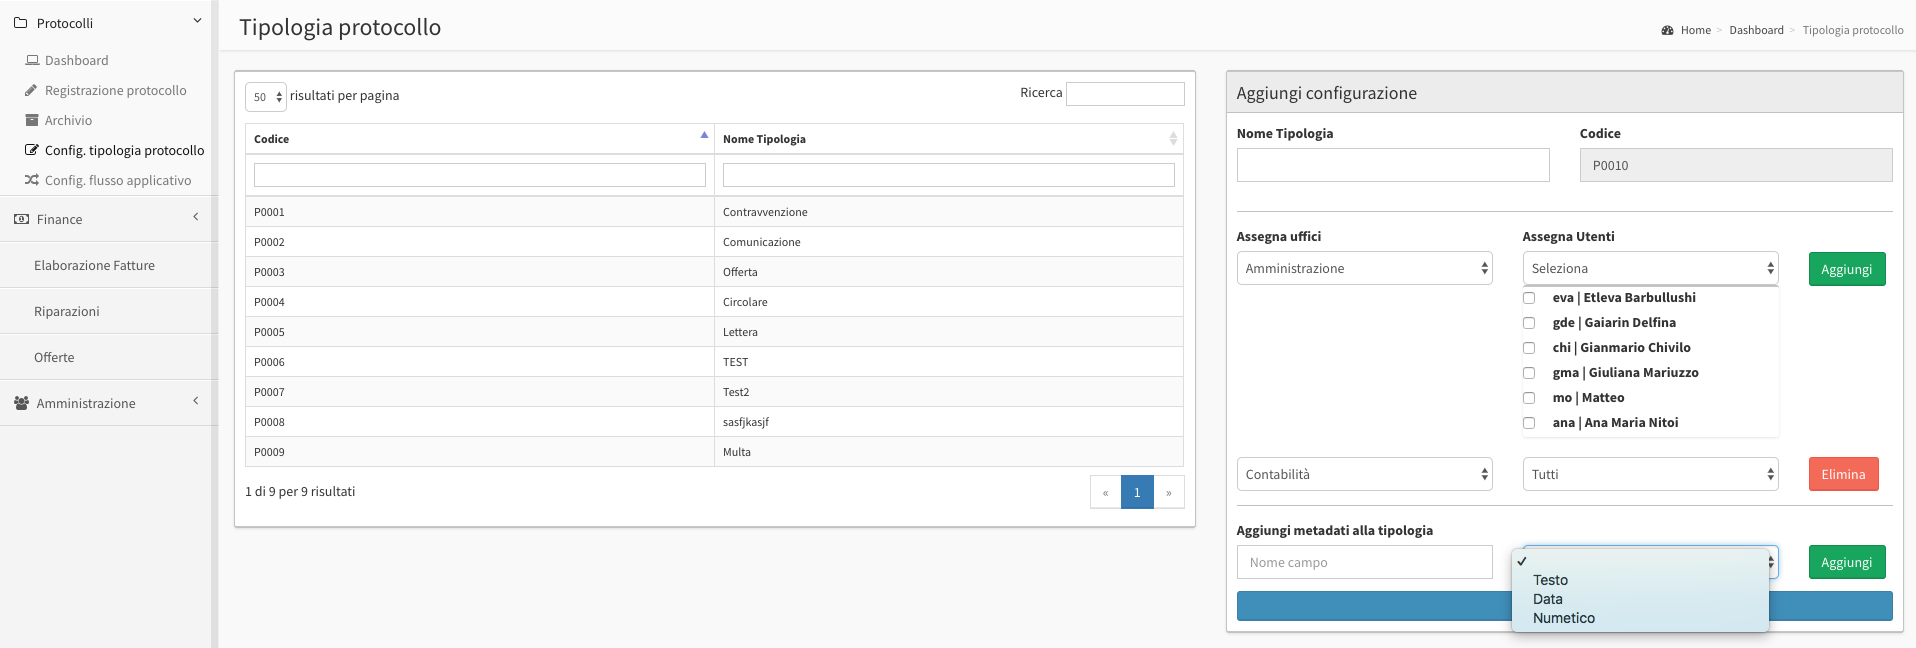
\includegraphics[width=\textwidth]{immagini/prodottofinito/configtipo.png}
            \caption{JQuery per selezione utenti}
        \end{figure}
        Con la precedente immagine è più facile visualizzare quanto precedentemente descritto.
        \\
        Lo stesso principio utilizzato nelle chiamate \textit{Ajax} precedentemente descritte è stato usato per aggiungere metadati a sostegno di una più arricchita descrizione della tipologia in fase di registrazione di un protocollo.
        
\subsection{Visualizzazione tipologia protocollo}
    \subsubsection{Codice}
        Dal punto di vista del codice non c'è nulla di nuovo rispetto alle pagine precedentemente descritte.
        \\
        I dati precedentemente inseriti vengono ora prelevati mediante apposta \textit{query} e stampati a video.
        \\
        È inoltre possibile modificare la configurazione dal punto di vista dei metadati utilizzando lo stesso sistema spiegato per la pagina precedente. 
        \\
        Per quanto riguarda gli operatori addetti, ad ogni modifica per un ufficio già esistente nella lista degli uffici coinvolti viene fatta una \textit{delete} di tutti gli operatori precedentemente inseriti e vengono caricati nel database quelli nuovi.
    \subsubsection{Resa finale}
        \begin{figure}[!h] 
            \centering 
            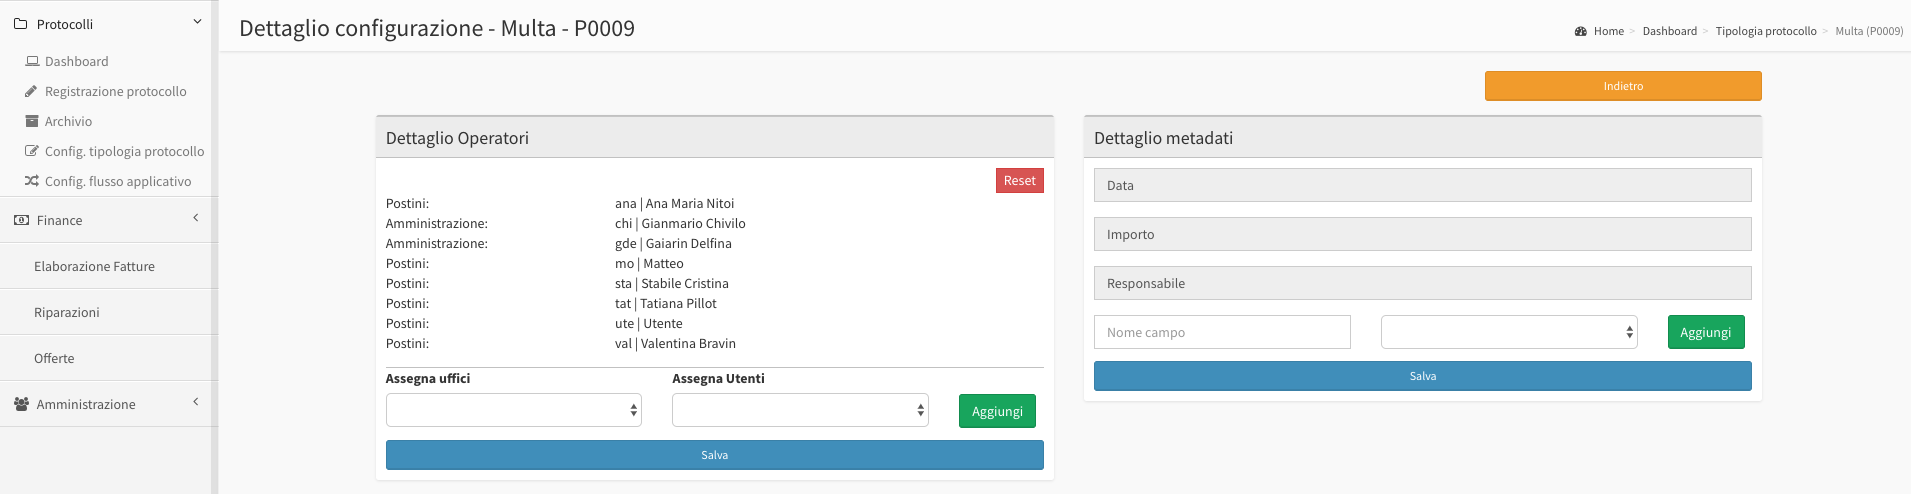
\includegraphics[width=\textwidth]{immagini/prodottofinito/dettaglioconfig.png}
            \caption{Dettaglio configurazione view}
        \end{figure}
        Con il tasto "Reset" è possibile eliminare tutti i gli operatori assegnati per poter riconfigurare da zero la tipologia. 
        \\ 
        Nel caso in cui non vi siano documenti collegati alla tipologia presa in esame, accanto al tasto "Indietro", sarà possibile visualizzare il tasto "Elimina" che consente l'eliminazione della tipologia creata. 
        
        

% !TEX encoding = UTF-8
% !TEX TS-program = pdflatex
% !TEX root = ../tesi.tex

%**************************************************************

\chapter{Verifica e validazione}
\label{cap:verifica-validazione}
%**************************************************************

\section{Verifica}

\subsection{Analisi statica}
L'analisi statica fa uso di tecniche che non richiedono l'esecuzione del prodotto software, mirando ad avere un indice di qualità del codice tramite la lettura.
\\
L'analisi statica è stata applicata per tutta la durata del periodo di codifica, nei seguenti modi:
\begin{itemize}
    \item rileggendo innanzitutto attentamente il codice prodotto durante tutta la fase di codifica, facendo uso di tecniche come \emph{walkthrough}\glsfirstoccur e \emph{inspection}\glsfirstoccur;
    
    \item tenendo sotto controllo la qualità del codice grazie a Psalm.
\end{itemize}

\subsection{Analisi dinamica}
L'analisi dinamica richiede l'esecuzione del prodotto software. Si avvale tipicamente di test progettati per essere utilizzabili nel momento in cui si effettua una modifica al software.
\\
Allo scopo di effettuare l'analisi dinamica, sono stati stesi ed effettuati dei test di unità sulle componenti, usando il framework per unit testing PHPUnit. 
\\
La procedura di unit testing e stata svolta nel seguente modo:
\begin{itemize}
    \item sono stati scritti dei brevi ma completi \textit{snippet} di codice che testino ogni funzionalità isolata, sia per quanto riguarda i casi di funzionamento corretto che quelli di funzionamento errato;
    
    \item sono stati raggruppati gli \textit{snippet} in TestCase;
    
    \item sono stati raggruppati i TestCase in TestSuite, che rappresentano una macro funzionalità rappresentata dal codice;
    
    \item infine è stato eseguito il codice di testing correggendo gli errori riscontrati ed assicurandosi che tutto il codice sia correttamente testato.
\end{itemize}

Sono stati inoltre eseguiti dei test funzionali, ovvero l'esecuzione dei casi d'uso previsti, simulando il comportamento atteso dall'utente, allo scopo di controllare che non si presentino bug o comportamenti imprevisti dell'applicazione.

\section{Validazione}
Lo scopo della validazione è accertare che il prodotto finale corrisponda alle attese, in modo da soddisfare tutti i requisiti prefissati inizialmente. I tipi di validazione effettuati sono stati due:
\begin{itemize}
    \item \textbf{validazione interna:} la validazione interna, chiamata anche "alfa test" o "pre-collaudo", è un processo che viene svolto da chi ha sviluppato il sistema. Al termine dello sviluppo del prodotto è stata effettuata la validazione interna in modo autonomo, simulando l'uso del prodotto da parte di un utente e verificando che tutte le funzionalità implementate funzionassero correttamente;
    
    \item \textbf{validazione esterna:} la validazione esterna, chiamata invece "beta-test" o "collaudo", è svolta dal committente del prodotto o dalla sua utenza. Il collaudo del prodotto sviluppato nel periodo di stage è stato fatto tramite una presentazione e dimostrazione dello stesso ai committenti.
\end{itemize}
% !TEX encoding = UTF-8
% !TEX TS-program = pdflatex
% !TEX root = ../tesi.tex

%**************************************************************
\chapter{Conclusioni}
\label{cap:conclusioni}
%**************************************************************
Quest'ultimo capitolo contiene un'analisi riassuntiva degli obiettivi raggiunti, delle conoscenze acquisite e le conclusioni sull'attività svolta.
%**************************************************************
\section{Obiettivi raggiunti}
Gli obiettivi prefissati nel piano di lavoro sono stati completamente raggiunti. Ogni giorno, in seguito all'analisi degli obiettivi raggiunti e delle problematiche da risolvere, veniva redatto un documento informale contenente a grandi linee le soluzioni che si intendevano intraprendere, concordatamene con il tutor aziendale.
\\
A livello tecnologico ho acquisito una buona padronanza dei linguaggi di sviluppo web quali PHP e JavaScript che per la mia futura carriera sono fondamentali. 

%**************************************************************
\section{Conoscenze acquisite}
Oltre a quanto detto sopra, la cosa più importante che ho imparato in questo stage è stata la capacità di realizzare codice il più possibile mantenibile e sicuro dal punto di vista delle vulnerabilità.
\\ 
Quest'ultimo punto è quello a mio avviso più importante e formativo per uno studente che si affaccia al mondo del lavoro e che come me vorrebbe affacciarsi al settore della sicurezza informatica.
%**************************************************************
\section{Conclusioni}
Personalmente ritengo questa esperienza di stage molto positiva e formativa, sotto
molti punti di vista.
\\
Innanzitutto mi ha permesso di affacciarmi al mondo del lavoro nell'ambito informatico per la prima volta: entrare in contatto con un team di professionisti del settore è un esperienza molto formativa che sicuramente non può essere insegnata in un contesto universitario. 
\\
Penso che un opportunità di stage come quella offerta dal nostro percorso di studi, di cui sono completamente soddisfatto, è fondamentale per mettere in pratica, e quindi comprendere ancora meglio, tutte le conoscenze teoriche apprese durante questi anni di studio.
\\
Sicuramente le nozioni insegnate dal corso di Laurea in Informatica, ma soprattutto il metodo di studio che viene comunicato, mi hanno permesso di imparare nuove tecnologie senza difficoltà e di affrontare nuove sfide senza paura. Questo percorso mi ha permesso anche di comprendere le regole aziendali, dal rispettare gli orari lavorativi fino alla pianificazione e al raggiungimento degli obiettivi, molto diverse dall'ambito universitario.
\\
Mi ritengo molto soddisfatto del lavoro svolto in quanto il prodotto sarà venduto all'azienda proponente e, da come mi è stato riferito dal tutor aziendale, sarà ripreso per adattarlo all'esigenza di realizzare un gestionale per la fatturazione elettronica.
\\
Concludo dicendo che questo percorso mi ha permesso di conoscere meglio me stesso, i
miei limiti, ma anche i miei punti di forza e le aspirazioni.
%**************************************************************

\chapter*{Glossario}
\label{cap:glossario}
%A

%B
\textbf{Backend}: Il backend è la parte di un software che elabora i dati generati dal frontend. Il backend incapsula la logica di elaborazione dei dati, e non interagisce direttamente con l’utilizzatore.
\\
\\
\textbf{Brainstorming}: L'espressione brainstorming, traducibile in lingua italiana come "assalto mentale" o "tempesta di cervelli", è una tecnica creativa di gruppo per far emergere idee volte alla risoluzione di un problema. Sinteticamente consiste, dato un problema, nell'organizzare una riunione in cui ogni partecipante propone liberamente soluzioni al problema, senza che nessuna di esse venga minimamente censurata. La critica ed eventuale selezione interverrà solo in un secondo tempo, terminata la seduta di brainstorming
\\
\\
\textbf{ERP}: significa Enterprise Resource Planning ("pianificazione delle risorse d'impresa"). Si tratta di un sistema di gestione che integra tutti i processi di business rilevanti di un'azienda (vendite, acquisti, gestione magazzino, contabilità ecc.).
\\
\\
%F
\textbf{Framework}: Un framework, in informatica e specificatamente nello sviluppo software, è un’architettura logica di supporto su cui un software può essere progettato e realizzato, spesso facilitandone lo sviluppo da parte del programmatore.
\\
\\
\textbf{Frontend}: Nel campo della progettazione software, il front-end è la parte di un sistema software che gestisce l’interazione con l’utente o con sistemi esterni che producono dati di ingresso.
\\
\\
%I
\textbf{IDE}: In informatica un ambiente di sviluppo integrato (in lingua inglese integrated development environment) è un software che, in fase di programmazione, aiuta i programmatori nello sviluppo del codice sorgente di un programma. Spesso l’IDE aiuta lo sviluppatore segnalando errori di sintassi del codice direttamente in fase di scrittura, oltre a tutta una serie di strumenti e funzionalità di supporto alla fase di sviluppo e debugging.
\\
\\
%J
\textbf{JSON}: (JavaScript Object Notation) Standard usato per trasmettere dati tramite lo
scambio di oggetti nei quali le informazioni sono salvate in coppie chiave-valore.
\\
\\
%M
\textbf{Metadato}:
informazioni aggiuntive che hanno attinenza con i documenti in fase di caricamento.
\\
\\
\textbf{MockFlow}:
MockFkow è un tool molto famoso per la sezione “Wireframe Pro“, ovvero un’applicazione concepita per la creazione di progetti di web design condivisibili con il team di lavoro. MockFlow è completamente interattivo e permette anche la realizzazione delle Sitemap delle pagine create. E’ possibile esportare in qualsiasi formato e fornisce una numerosa quantità di funzioni e strumenti.
\\
\\
%P
\textbf{PHP}: è un linguaggio di scripting interpretato, originariamente concepito per la programmazione di pagine web dinamiche.
\\
\\
\textbf{Plugin}: è un componente software che aggiunge specifiche funzionalità ad un programma esistente.
\\
\\
%R
\textbf{Refractoring}: in ingegneria del software, il refactoring (o code-refactoring) è una "tecnica strutturata per modificare la struttura interna di porzioni di codice senza modificarne il comportamento esterno", applicata per migliorare alcune caratteristiche non funzionali del software.
\\
\\
%S
\textbf{Software House}: azienda che si occupa dell'elaborazione e della commercializzazione di programmi per elaboratori.
\\
\\
\textbf{Software Intergration}: combinazione di subroutine, moduli software o programmi completi con altri componenti software per sviluppare un'applicazione o migliorare la funzionalità di uno esistente. Spesso richiedendo molte modifiche al codice sorgente, gli sviluppatori, così come il personale IT, possono dedicare gran parte del loro tempo a realizzare l'integrazione del software.
\\
\\
%U
\textbf{UML}: In ingegneria del software UML, Unified Modeling Language (ing. linguaggio di modellazione unificato) è un linguaggio di modellazione e specifica basato sul paradigma object-oriented. L’UML svolge un’importantissima funzione di “lingua franca” nella comunità della progettazione e programmazione a oggetti. Gran parte della letteratura di settore usa tale linguaggio per descrivere soluzioni analitiche e progettuali in modo sintetico e comprensibile a un vasto pubblico.
\\
\\
\textbf{XML}: è un metalinguaggio per la definizione di linguaggi di markup, ovvero un linguaggio marcatore basato su un meccanismo sintattico che consente di definire e controllare il significato degli elementi contenuti in un documento o in un testo.
%\appendix
%\input{capitoli/capitolo-A}

%**************************************************************
% Materiale finale
%**************************************************************
\backmatter
\printglossaries
% !TEX encoding = UTF-8
% !TEX TS-program = pdflatex
% !TEX root = ../tesi.tex

%**************************************************************
% Bibliografia
%**************************************************************

\cleardoublepage
\chapter{Bibliografia}

\nocite{*}

% Stampa i siti web consultati
\printbibliography[heading=subbibliography,title={Siti web consultati},type=online]

\end{document}
